% Options for packages loaded elsewhere
\PassOptionsToPackage{unicode}{hyperref}
\PassOptionsToPackage{hyphens}{url}
%
\documentclass[
]{book}
\title{Apéndices del Libro Pobreza y Desigualdad en R}
\author{Bonavida, Cristian - CEDLAS\footnote{Para explorar una posible manera de plotear histogramas de frecuencia relativa o absoluta junto con un densidad suavizada el lector encontrará util la \href{https://stackoverflow.com/questions/27611438/density-curve-overlay-on-histogram-where-vertical-axis-is-frequency-aka-count}{siguiente entrada} de \emph{stackoverflow}.} \and Laguinge, Luis - CEDLAS\footnote{Para los usuarios que no esten tan familiarizados con las nociones de \emph{Environment} y \emph{Non-Standard Evaluation} se recomienda revisar las siguientes referencias para un tratamiento mas detallado.

  *\url{http://adv-r.had.co.nz/Environments.html\#environments}

  *\url{http://adv-r.had.co.nz/Computing-on-the-language.html}

  *\url{https://advanced-r-solutions-ed1.netlify.app/non-standard-evaluation.html\#non-standard-evaluation-in-subse}} \and Varvasino, Joaquín - CEDLAS\footnote{\textbf{Joaquín} estudió la Licenciatura y la Maestría en Economía (UNLP). Actualmente trabaja como investigador en CEDLAS en temas de desigualdad y mercado laboral. Para entrar en contacto podes escribirle a \href{mailto:joaquinvarvasino@hotmail.com}{\nolinkurl{joaquinvarvasino@hotmail.com}}. Para conocer más de Joaquín, sus proyectos y publicaciones podes visitar su perfil en \href{https://twitter.com/mynameisjoaco}{twitter} o \href{https://www.linkedin.com/in/joaquin-varvasino-826819135/}{linkedin}}}
\date{}

\usepackage{amsmath,amssymb}
\usepackage{lmodern}
\usepackage{iftex}
\ifPDFTeX
  \usepackage[T1]{fontenc}
  \usepackage[utf8]{inputenc}
  \usepackage{textcomp} % provide euro and other symbols
\else % if luatex or xetex
  \usepackage{unicode-math}
  \defaultfontfeatures{Scale=MatchLowercase}
  \defaultfontfeatures[\rmfamily]{Ligatures=TeX,Scale=1}
\fi
% Use upquote if available, for straight quotes in verbatim environments
\IfFileExists{upquote.sty}{\usepackage{upquote}}{}
\IfFileExists{microtype.sty}{% use microtype if available
  \usepackage[]{microtype}
  \UseMicrotypeSet[protrusion]{basicmath} % disable protrusion for tt fonts
}{}
\makeatletter
\@ifundefined{KOMAClassName}{% if non-KOMA class
  \IfFileExists{parskip.sty}{%
    \usepackage{parskip}
  }{% else
    \setlength{\parindent}{0pt}
    \setlength{\parskip}{6pt plus 2pt minus 1pt}}
}{% if KOMA class
  \KOMAoptions{parskip=half}}
\makeatother
\usepackage{xcolor}
\IfFileExists{xurl.sty}{\usepackage{xurl}}{} % add URL line breaks if available
\IfFileExists{bookmark.sty}{\usepackage{bookmark}}{\usepackage{hyperref}}
\hypersetup{
  pdftitle={Apéndices del Libro Pobreza y Desigualdad en R},
  pdfauthor={Bonavida, Cristian - CEDLAS; Laguinge, Luis - CEDLAS; Varvasino, Joaquín - CEDLAS},
  hidelinks,
  pdfcreator={LaTeX via pandoc}}
\urlstyle{same} % disable monospaced font for URLs
\usepackage{color}
\usepackage{fancyvrb}
\newcommand{\VerbBar}{|}
\newcommand{\VERB}{\Verb[commandchars=\\\{\}]}
\DefineVerbatimEnvironment{Highlighting}{Verbatim}{commandchars=\\\{\}}
% Add ',fontsize=\small' for more characters per line
\usepackage{framed}
\definecolor{shadecolor}{RGB}{248,248,248}
\newenvironment{Shaded}{\begin{snugshade}}{\end{snugshade}}
\newcommand{\AlertTok}[1]{\textcolor[rgb]{0.94,0.16,0.16}{#1}}
\newcommand{\AnnotationTok}[1]{\textcolor[rgb]{0.56,0.35,0.01}{\textbf{\textit{#1}}}}
\newcommand{\AttributeTok}[1]{\textcolor[rgb]{0.77,0.63,0.00}{#1}}
\newcommand{\BaseNTok}[1]{\textcolor[rgb]{0.00,0.00,0.81}{#1}}
\newcommand{\BuiltInTok}[1]{#1}
\newcommand{\CharTok}[1]{\textcolor[rgb]{0.31,0.60,0.02}{#1}}
\newcommand{\CommentTok}[1]{\textcolor[rgb]{0.56,0.35,0.01}{\textit{#1}}}
\newcommand{\CommentVarTok}[1]{\textcolor[rgb]{0.56,0.35,0.01}{\textbf{\textit{#1}}}}
\newcommand{\ConstantTok}[1]{\textcolor[rgb]{0.00,0.00,0.00}{#1}}
\newcommand{\ControlFlowTok}[1]{\textcolor[rgb]{0.13,0.29,0.53}{\textbf{#1}}}
\newcommand{\DataTypeTok}[1]{\textcolor[rgb]{0.13,0.29,0.53}{#1}}
\newcommand{\DecValTok}[1]{\textcolor[rgb]{0.00,0.00,0.81}{#1}}
\newcommand{\DocumentationTok}[1]{\textcolor[rgb]{0.56,0.35,0.01}{\textbf{\textit{#1}}}}
\newcommand{\ErrorTok}[1]{\textcolor[rgb]{0.64,0.00,0.00}{\textbf{#1}}}
\newcommand{\ExtensionTok}[1]{#1}
\newcommand{\FloatTok}[1]{\textcolor[rgb]{0.00,0.00,0.81}{#1}}
\newcommand{\FunctionTok}[1]{\textcolor[rgb]{0.00,0.00,0.00}{#1}}
\newcommand{\ImportTok}[1]{#1}
\newcommand{\InformationTok}[1]{\textcolor[rgb]{0.56,0.35,0.01}{\textbf{\textit{#1}}}}
\newcommand{\KeywordTok}[1]{\textcolor[rgb]{0.13,0.29,0.53}{\textbf{#1}}}
\newcommand{\NormalTok}[1]{#1}
\newcommand{\OperatorTok}[1]{\textcolor[rgb]{0.81,0.36,0.00}{\textbf{#1}}}
\newcommand{\OtherTok}[1]{\textcolor[rgb]{0.56,0.35,0.01}{#1}}
\newcommand{\PreprocessorTok}[1]{\textcolor[rgb]{0.56,0.35,0.01}{\textit{#1}}}
\newcommand{\RegionMarkerTok}[1]{#1}
\newcommand{\SpecialCharTok}[1]{\textcolor[rgb]{0.00,0.00,0.00}{#1}}
\newcommand{\SpecialStringTok}[1]{\textcolor[rgb]{0.31,0.60,0.02}{#1}}
\newcommand{\StringTok}[1]{\textcolor[rgb]{0.31,0.60,0.02}{#1}}
\newcommand{\VariableTok}[1]{\textcolor[rgb]{0.00,0.00,0.00}{#1}}
\newcommand{\VerbatimStringTok}[1]{\textcolor[rgb]{0.31,0.60,0.02}{#1}}
\newcommand{\WarningTok}[1]{\textcolor[rgb]{0.56,0.35,0.01}{\textbf{\textit{#1}}}}
\usepackage{longtable,booktabs,array}
\usepackage{calc} % for calculating minipage widths
% Correct order of tables after \paragraph or \subparagraph
\usepackage{etoolbox}
\makeatletter
\patchcmd\longtable{\par}{\if@noskipsec\mbox{}\fi\par}{}{}
\makeatother
% Allow footnotes in longtable head/foot
\IfFileExists{footnotehyper.sty}{\usepackage{footnotehyper}}{\usepackage{footnote}}
\makesavenoteenv{longtable}
\usepackage{graphicx}
\makeatletter
\def\maxwidth{\ifdim\Gin@nat@width>\linewidth\linewidth\else\Gin@nat@width\fi}
\def\maxheight{\ifdim\Gin@nat@height>\textheight\textheight\else\Gin@nat@height\fi}
\makeatother
% Scale images if necessary, so that they will not overflow the page
% margins by default, and it is still possible to overwrite the defaults
% using explicit options in \includegraphics[width, height, ...]{}
\setkeys{Gin}{width=\maxwidth,height=\maxheight,keepaspectratio}
% Set default figure placement to htbp
\makeatletter
\def\fps@figure{htbp}
\makeatother
\setlength{\emergencystretch}{3em} % prevent overfull lines
\providecommand{\tightlist}{%
  \setlength{\itemsep}{0pt}\setlength{\parskip}{0pt}}
\setcounter{secnumdepth}{5}
\usepackage{booktabs}
\ifLuaTeX
  \usepackage{selnolig}  % disable illegal ligatures
\fi
\usepackage[]{natbib}
\bibliographystyle{plainnat}

\begin{document}
\maketitle

{
\setcounter{tocdepth}{1}
\tableofcontents
}
\hypertarget{bienvenidos}{%
\chapter{Bienvenidos}\label{bienvenidos}}

\hypertarget{sobre-este-proyecto}{%
\section*{Sobre este Proyecto:}\label{sobre-este-proyecto}}
\addcontentsline{toc}{section}{Sobre este Proyecto:}

Nos propusimos trasncribir al lenguaje R y Python los apéndices del libro ``Pobreza y Desigualdad en América Latina'' de Gasparini, Cicowiez y Sosa Escudero que originalmente fueron escritos para Stata y que permitían replicar los datos e información presentados por los autores en el texto. Cada capítulo consta de un apéndice con códigos que permiten llevar a la práctica los conceptos desarrollados. Aquí \textbf{los traducimos a nuevos lenguajes y los presentamos en un formato amigable para permitir que un público más amplio y de diversas disciplinas pueda aprovecharlos}.

El objetivo de este mini-proyecto no es otro que poner a disposición de un público más amplio estas herramientas útiles y mantener actualizado un material único, que ayuda a adentrarse y trabajar sobre la temática de pobreza y desigualdad. Es por eso que este material es de carácter complementario a las explicaciones y detalles conceptuales que se presentan en el libro de texto y los apéndices.

\hypertarget{el-libro}{%
\section*{El Libro}\label{el-libro}}
\addcontentsline{toc}{section}{El Libro}

Si esta es la primera vez que te encontrás con este libro, antes de empezar con los códigos, dejanos presentartelo.

El propósito del libro es ayudar al lector interesado en América Latina a que recorra el arduo camino entre los datos y el reporte de resultados rigurosos que puedan contribuir al debate sobre la pobreza y la desigualdad en la región. El volumen busca poner al alcance del lector un conjunto de instrumentos que lo motiven hacia la investigación empírica, y que le permitan producir resultados de la manera más rigurosa posible, para así contribuir a los objetivos últimos de explicar y cambiar la realidad social de la región. Las discusiones conceptuales y analíticas son ilustradas con ejemplos concretos construidos con datos de los países de la región.

\begin{center}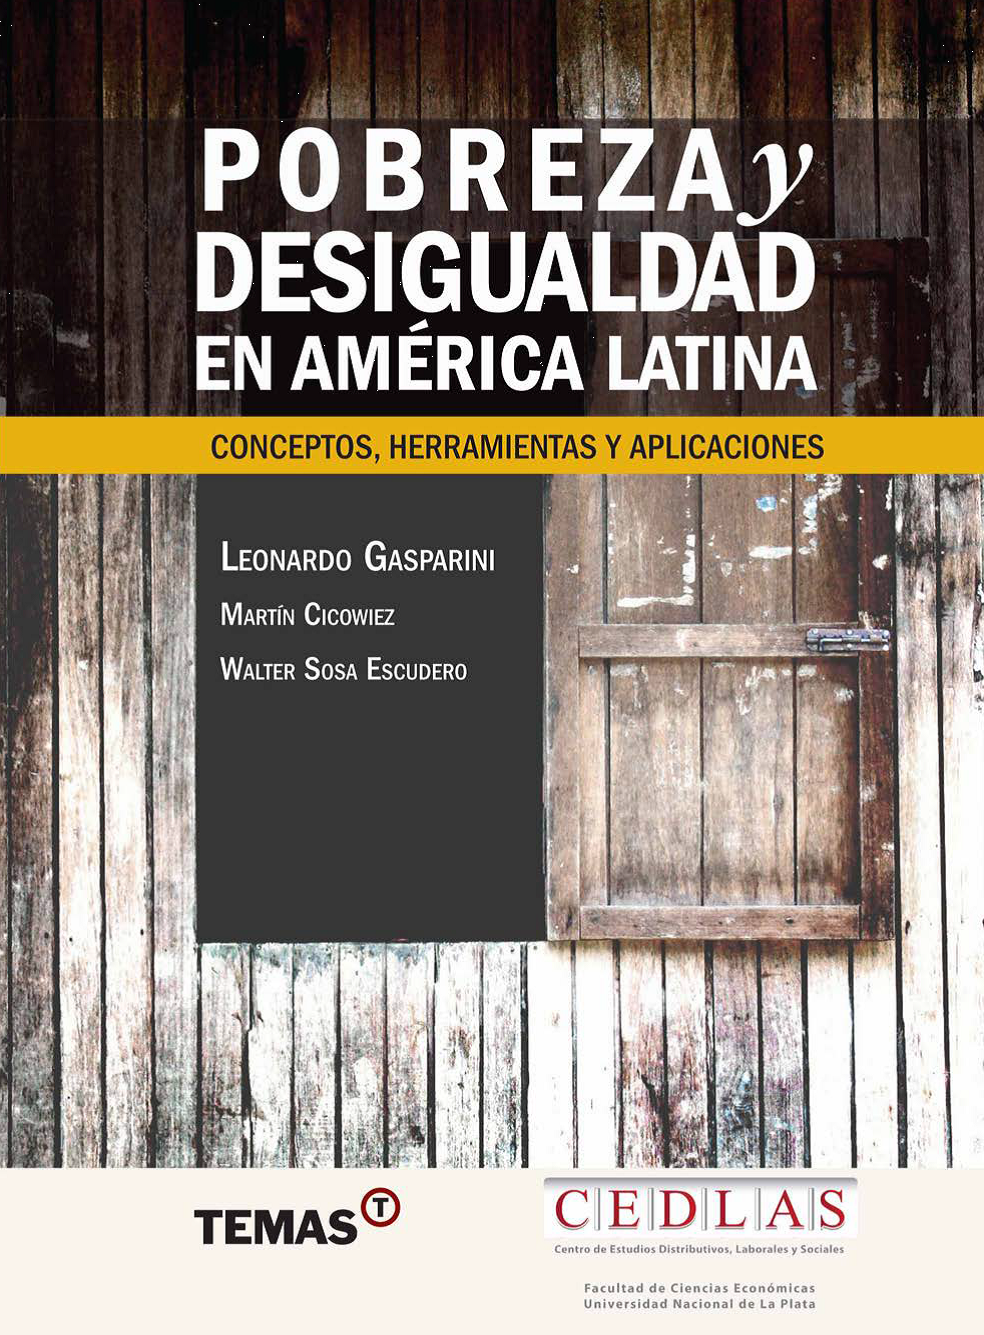
\includegraphics[width=0.6\linewidth]{portada_libro} \end{center}

Una enorme ventaja de este trabajo es que se encuentra disponible para todos, ya que se lo puede descargar gratuitamente desde el la \href{https://www.cedlas.econo.unlp.edu.ar/wp/publicaciones/libros/pobreza-y-desigualdad-en-america-latina/}{página del libro}. Te invitamos a que puedas recorrerlo, leerlo y dedicarle varios minutos antes de adentrarte en las próximas secciones.

\hypertarget{cuxf3mo-aprovechar-este-material}{%
\section*{Cómo aprovechar este material}\label{cuxf3mo-aprovechar-este-material}}
\addcontentsline{toc}{section}{Cómo aprovechar este material}

Un punto importante es que estos códigos que te presentamos están atados a los contenidos y explicaciones que se desarrollan a lo largo de los capítulos del libro. Por eso notarás que los códigos no son autocontenidos al 100\%, es decir si bien refuerzan las ideas principales detrás de cada indicador, de cada gráfico o cada estimación, y están acompañados de instrucciones generales, no cubren en profundidad los conceptos teóricos e incluso prácticos detrás de su uso. Por es que decimos que \textbf{este material es de carácter complementario a las explicaciones y detalles conceptuales que se presentan en el libro de texto y los apéndices}. Para aprovecharlas al máximo te recomendamos tener abierta junto con la pestaña de R o Python, el pdf del libro de texto para ir siguiendo capitulo a capitulo los contenidos. De esta forma no solo será posible replicar las estimaciones sino también comprenderlas y saber entender qué nos dicen y qué no nos dicen.

\hypertarget{quuxe9-es-y-quuxe9-no-es}{%
\section*{Qué es y qué no es}\label{quuxe9-es-y-quuxe9-no-es}}
\addcontentsline{toc}{section}{Qué es y qué no es}

Es importante fijar las expectativas desde el principio. En estos códigos vas a encontrar mucha información y muchos temas a cubrir, mientras que otros nos quedarán para una próxima entrega. En este sentido, este material \textbf{no busca ser una guía exhaustiva a modo de tutorial para iniciarse en el lenguaje de programación}. El propósito será seguir los códigos presentados en los apéndices del libro con la misma estructura temática y con el objetivo de facilitar nuevas herramientas al usuario en base a los que ya fue escrito. Por lo que si bien el material es útil para entrenarse en este lenguaje, es más bien un proyecto que permite expandir sobre conocimientos y nociones previas. Es por eso que se recomienda que el lector ya esté algo familiarizado con la sintaxis y el programa. Si no este no es tu caso, no te preocupes!, te vamos a dejar a continuación varias referencias para que puedas entrar en calor y ponerte a punto antes de empezar.

\begin{itemize}
\item
  Tutoriales para inciarse en R

  \begin{itemize}
  \item
    \url{https://martinmontane.github.io/CienciaDeDatosBook/index.html}
  \item
    \url{https://diegokoz.github.io/Curso_R_EPH_clases/}
  \end{itemize}
\item
  Para hacer el camino desde Stata

  \begin{itemize}
  \tightlist
  \item
    \url{https://www.matthieugomez.com/statar/index.html}
  \end{itemize}
\end{itemize}

\hypertarget{quuxe9-necesitamos-antes-de-arrancar}{%
\section*{Qué necesitamos antes de arrancar}\label{quuxe9-necesitamos-antes-de-arrancar}}
\addcontentsline{toc}{section}{Qué necesitamos antes de arrancar}

Para poder seguir los códigos que te presentamos vas a necesitar descargarte (o al menos tener acceso) a las bases de datos sobre las que iremos trabajando. Estas bases de datos son las encuestas que desarrolla cada país y que el CEDLAS sistematiza para ofrecerlas en un formato usable para los investigadores. En el siguiente \href{https://www.cedlas.econo.unlp.edu.ar/wp/publicaciones/libros/pobreza-y-desigualdad-en-america-latina/\#1505501369949-15c93bca-b4f8}{link} encontrarás el repositorio.

~

\hypertarget{capuxedtulo-2}{%
\chapter{Capítulo 2}\label{capuxedtulo-2}}

\hypertarget{herramientas-para-el-anuxe1lisis-distributivo}{%
\section*{Herramientas para el análisis distributivo}\label{herramientas-para-el-anuxe1lisis-distributivo}}

\hypertarget{escrito-por-cristian-bonavida}{%
\subsubsection*{Escrito por: Cristian Bonavida}\label{escrito-por-cristian-bonavida}}
\addcontentsline{toc}{subsubsection}{Escrito por: Cristian Bonavida}

\hypertarget{last-update-0272021}{%
\subsubsection*{Last Update: 02/7/2021}\label{last-update-0272021}}
\addcontentsline{toc}{subsubsection}{Last Update: 02/7/2021}

~

\emph{Códigos escritos en base a los apéndices del libro ``Pobreza y Desigualdad en América Latina'' de Gasparini, Cicowiez y Sosa Escudero. El objeto de este material es reproducir la rutina de códigos para STATA presentada en el libro al lenguaje R. Este material es solo de caracter complementario a las explicaciones y detalles conceptuales que se presentan en el libro de texto y los apéndices}

~

\hypertarget{set-inicial}{%
\section*{Set Inicial}\label{set-inicial}}
\addcontentsline{toc}{section}{Set Inicial}

Cargo las librerias, limpio environment, defino el path y atajo para función paste

\begin{Shaded}
\begin{Highlighting}[]
\FunctionTok{library}\NormalTok{(dplyr)}
\FunctionTok{library}\NormalTok{(tidyverse) }\CommentTok{\# Data wrangling}
\FunctionTok{library}\NormalTok{(tidygraph)}
\FunctionTok{library}\NormalTok{(readxl)}
\FunctionTok{library}\NormalTok{(ggplot2)}
\FunctionTok{library}\NormalTok{(foreign)}
\FunctionTok{library}\NormalTok{(Hmisc)}

\FunctionTok{rm}\NormalTok{(}\AttributeTok{list=}\FunctionTok{ls}\NormalTok{())    }\CommentTok{\#empiezo limpiando todo }

\StringTok{"\%+\%"} \OtherTok{\textless{}{-}} \ControlFlowTok{function}\NormalTok{(x,y) }\FunctionTok{paste}\NormalTok{(x,y,}\AttributeTok{sep =} \StringTok{""}\NormalTok{)      }\CommentTok{\# defino un shorcut parar concat de texto}
\NormalTok{data\_dir }\OtherTok{\textless{}{-}} \StringTok{"C:/Users/HP/Desktop/CEDLAS {-} UNLP/Apendices en R/Material libro/encuestas{-}cedlas/Encuestas/"}  \CommentTok{\#seteo directorio }
\end{Highlighting}
\end{Shaded}

~

\hypertarget{introducciuxf3n-ejemplo-brasil}{%
\section{Introducción: ejemplo Brasil}\label{introducciuxf3n-ejemplo-brasil}}

\#\#\#- (pág. 72)

El siguiente código es introductorio y busca guiar al lector en la sintaxis básica a utilizar, mostrando a modo de ejemplo cómo replicar los resultados correspondientes al cuadro 2.1 del texto.

Como será al inicio de cada capítulo, el primer paso es obtener base de datos, en ese caso la versión procesada de la PNAD (Pesquisa Nacional por Amostra de Domicílios) de Brasil para el año 2007, accesible desde el link de descarga indicado en la sección anterior: datos y set up básico. (Añadir sección y referir allí)

Una vez descargada la encuesta y guardada en el directorio que el lector indicó al definir el objeto \emph{``data\_dir''} se carga la encuesta que se encuentra en formato STATA con la librería \texttt{foreing}. Dentro de ella el comando \texttt{read.dta()} permite importar en R bases de datos que están en formatos compatibles con otros programas o lenguajes. Las encuestas de hogares procesadas que se utilizan a lo largo del libro solo deben contener observaciones que denominamos coherentes, que en pocas palabras se trata de observaciones válidas que utilizamos en el cálculo de los ingresos familiares. Por ello siempre que se cargue una base luego se debe filtrarla a partir de la columna \emph{cohh}, para quedarse solo con estas observaciones.

Las encuestas de hogares, al igual que cualquier otra base de datos, se organizan en R como objetos tipo tabla que reciben el nombre de \texttt{dataframe}, donde las filas representan observaciones o registros y las columnas variables o campos. Con el comando \texttt{head()} podemos explorar las primeras observaciones de la encuesta. La expresión \texttt{{[},1:9{]}} indica incluir solo de la columna 1 a 9 para que el output no sea demasiado extenso.

\begin{Shaded}
\begin{Highlighting}[]
\CommentTok{\#cargo base}
\NormalTok{bra07 }\OtherTok{\textless{}{-}} \FunctionTok{read.dta}\NormalTok{(data\_dir }\SpecialCharTok{\%+\%} \StringTok{"Bra/2007/Bases/bra07\_cedlas.dta"}\NormalTok{) }\SpecialCharTok{\%\textgreater{}\%} 
         \FunctionTok{filter}\NormalTok{(cohh}\SpecialCharTok{==}\DecValTok{1}\NormalTok{)}

\FunctionTok{head}\NormalTok{(bra07[,}\DecValTok{1}\SpecialCharTok{:}\DecValTok{9}\NormalTok{])}
\end{Highlighting}
\end{Shaded}

\begin{verbatim}
##   edad relacion tarea hstrp pondera pais  ano  encuesta id
## 1   73        1    NA    NA     239  bra 2007 PNAD-2007 14
## 2   52        1    NA    NA     238  bra 2007 PNAD-2007 16
## 3   10        4    NA    NA     238  bra 2007 PNAD-2007 16
## 4   34        1    NA    NA     238  bra 2007 PNAD-2007 34
## 5   11        3    NA    NA     238  bra 2007 PNAD-2007 34
## 6   20        4    NA    NA     238  bra 2007 PNAD-2007 34
\end{verbatim}

A su vez, por tratarse de una encuesta, cada observación representa a varios individuos, tantos como indica el factor de expansión o variable de ponderación. En nuestro caso, todas las encuestas que utilizaremos contienen una variable de nombre \emph{pondera} que almacena el factor de expansión. Para más detalles sobre el uso de ponderadores, consultar más adelante la \protect\hyperlink{cap-3.6}{sección 3.6}

Para expandir las observaciones por su peso muestral debemos emplear alguna de las librerías disponibles creadas para tal fin, ya que ``por default'' los comandos base de R no estiman estadísticos ponderados, como es el caso por ejemplo del comando \texttt{summary()}. Si se comparan los valores que arroja respecto a los valores de los mismos estadísticos pero ponderados, es evidente que existen diferencias (excepto obviamente para el mínimo y el máximo). Existen varias librerías que nos permiten obtener descriptivos ponderados, aquí se presentan los resultados con el uso de \texttt{Hmisc}, pero también puede explorarse de forma similar las librerías \texttt{TAM} y \texttt{srvy}.

\begin{Shaded}
\begin{Highlighting}[]
\CommentTok{\#summary no arroja estadísticas descriptivas ponderadas}
\FunctionTok{summary}\NormalTok{(bra07}\SpecialCharTok{$}\NormalTok{ipcf)}
\end{Highlighting}
\end{Shaded}

\begin{verbatim}
##    Min. 1st Qu.  Median    Mean 3rd Qu.    Max.    NA's 
##     0.0   157.5   310.0   559.1   590.0 66000.0    1057
\end{verbatim}

\begin{Shaded}
\begin{Highlighting}[]
\CommentTok{\#replicar la información que nos da summary pero ponderandola {-} usando libreria Hmisc}
\FunctionTok{wtd.mean}\NormalTok{(bra07}\SpecialCharTok{$}\NormalTok{ipcf, }\AttributeTok{w=}\NormalTok{bra07}\SpecialCharTok{$}\NormalTok{pondera)}
\end{Highlighting}
\end{Shaded}

\begin{verbatim}
## [1] 574.3455
\end{verbatim}

\begin{Shaded}
\begin{Highlighting}[]
\FunctionTok{wtd.quantile}\NormalTok{(bra07}\SpecialCharTok{$}\NormalTok{ipcf, }\AttributeTok{probs =}\FunctionTok{c}\NormalTok{(}\FloatTok{0.25}\NormalTok{, }\FloatTok{0.50}\NormalTok{, }\FloatTok{0.75}\NormalTok{) , }\AttributeTok{w=}\NormalTok{bra07}\SpecialCharTok{$}\NormalTok{pondera)}
\end{Highlighting}
\end{Shaded}

\begin{verbatim}
##   25%   50%   75% 
## 165.0 330.0 621.5
\end{verbatim}

\begin{Shaded}
\begin{Highlighting}[]
\FunctionTok{min}\NormalTok{(bra07}\SpecialCharTok{$}\NormalTok{ipcf, }\AttributeTok{na.rm =}\NormalTok{T)}
\end{Highlighting}
\end{Shaded}

\begin{verbatim}
## [1] 0
\end{verbatim}

\begin{Shaded}
\begin{Highlighting}[]
\FunctionTok{max}\NormalTok{(bra07}\SpecialCharTok{$}\NormalTok{ipcf, }\AttributeTok{na.rm =}\NormalTok{T)}
\end{Highlighting}
\end{Shaded}

\begin{verbatim}
## [1] 66000
\end{verbatim}

Mientras que la media no pondera es de 559.1 al ponderar el valor estimado es 574.3
Lo mismo ocurre para la mediana, el primer y el tercer cuartil de la distribución.

Una opción recomendada para usuarios más familiarizados con la sintaxis de R, es definir una función que nos calcule e imprima los resultados para estos estadísticos ponderados de una sola vez, replicando lo que hace \texttt{summary()}. Las funciones son una especie de comando personalizado que nos permiten customizar los cálculos y el output a nuestra necesidad o gusto. -ver \protect\hyperlink{cap-3.2}{capitulo siguiente} donde nos extendemos sobre el uso de funciones-. En este caso nos permite elegir qué estadisticos queremos calcular y cómo mostrarlos, con una salida que incluye un título junto al resultado númerico mediante la función \texttt{paste()}) y redondeando a un decimal (mediante la función \texttt{round(...,\ d=1)})

\begin{Shaded}
\begin{Highlighting}[]
\NormalTok{my\_weighted\_stats }\OtherTok{\textless{}{-}} \ControlFlowTok{function}\NormalTok{(argumento1, argumento2)\{}
  
  \FunctionTok{print}\NormalTok{(}\FunctionTok{paste}\NormalTok{(}\StringTok{"Mean:"}\NormalTok{, }\FunctionTok{round}\NormalTok{( }\FunctionTok{wtd.mean}\NormalTok{(argumento1, }\AttributeTok{w=}\NormalTok{argumento2), }\AttributeTok{d=}\DecValTok{1}\NormalTok{ )))}
  \FunctionTok{print}\NormalTok{(}\FunctionTok{paste}\NormalTok{(}\StringTok{"Sd:"}\NormalTok{, }\FunctionTok{round}\NormalTok{( }\FunctionTok{sqrt}\NormalTok{(}\FunctionTok{wtd.var}\NormalTok{(argumento1, }\AttributeTok{w=}\NormalTok{argumento2)), }\AttributeTok{d=}\DecValTok{1}\NormalTok{ )))}
  \FunctionTok{print}\NormalTok{(}\FunctionTok{round}\NormalTok{( }\FunctionTok{wtd.quantile}\NormalTok{(bra07}\SpecialCharTok{$}\NormalTok{ipcf, }\AttributeTok{probs =}\FunctionTok{c}\NormalTok{(}\FloatTok{0.25}\NormalTok{, }\FloatTok{0.50}\NormalTok{, }\FloatTok{0.75}\NormalTok{) , }\AttributeTok{w=}\NormalTok{bra07}\SpecialCharTok{$}\NormalTok{pondera), }\AttributeTok{d=}\DecValTok{1}\NormalTok{ ))}
  \FunctionTok{print}\NormalTok{(}\FunctionTok{paste}\NormalTok{(}\StringTok{"Min:"}\NormalTok{, }\FunctionTok{round}\NormalTok{( }\FunctionTok{min}\NormalTok{(argumento1, }\AttributeTok{na.rm=}\ConstantTok{TRUE}\NormalTok{), }\AttributeTok{d=}\DecValTok{1}\NormalTok{ )))}
  \FunctionTok{print}\NormalTok{(}\FunctionTok{paste}\NormalTok{(}\StringTok{"Max:"}\NormalTok{, }\FunctionTok{round}\NormalTok{( }\FunctionTok{max}\NormalTok{(argumento1, }\AttributeTok{na.rm=}\ConstantTok{TRUE}\NormalTok{), }\AttributeTok{d=}\DecValTok{1}\NormalTok{ )))}
  
\NormalTok{\}}
\end{Highlighting}
\end{Shaded}

Una vez definida la función debemos llamarla por el nombre indicando sus argumentos. En este caso el primero hace referencia a la variable y el segundo al ponderador. La función devuelve la información que arrojaría el comando \texttt{summ} en STATA ponderando las estimaciones.

\begin{Shaded}
\begin{Highlighting}[]
\FunctionTok{my\_weighted\_stats}\NormalTok{(bra07}\SpecialCharTok{$}\NormalTok{ipcf, bra07}\SpecialCharTok{$}\NormalTok{pondera)}
\end{Highlighting}
\end{Shaded}

\begin{verbatim}
## [1] "Mean: 574.3"
## [1] "Sd: 970.2"
##   25%   50%   75% 
## 165.0 330.0 621.5 
## [1] "Min: 0"
## [1] "Max: 66000"
\end{verbatim}

Una de las principales ventajas de las funciones es que nos permiten replicar los resultados para distintas encuestas o también para distintos subconjuntos de los datos. Por ejemplo, en el caso de la PNAD 2007 de Brasil, la variable \emph{region} puede tomar los valores 1, 2, 3, 4 o 5 dependiendo de si la observación corresponde a la región Norte, Nordeste, Sudeste, Sur o Centro-Oeste, respectivamente. Así, las líneas siguientes pueden utilizarse para computar los estadísticos para dichas regiones, replicando aquí las columnas ``Norte'' y ``Nordeste'' del cuadro 2.1

\begin{Shaded}
\begin{Highlighting}[]
\FunctionTok{my\_weighted\_stats}\NormalTok{(bra07}\SpecialCharTok{$}\NormalTok{ipcf[bra07}\SpecialCharTok{$}\NormalTok{region}\SpecialCharTok{==}\DecValTok{1}\NormalTok{], bra07}\SpecialCharTok{$}\NormalTok{pondera[bra07}\SpecialCharTok{$}\NormalTok{region}\SpecialCharTok{==}\DecValTok{1}\NormalTok{])}
\end{Highlighting}
\end{Shaded}

\begin{verbatim}
## [1] "Mean: 391"
## [1] "Sd: 753.6"
##   25%   50%   75% 
## 165.0 330.0 621.5 
## [1] "Min: 0"
## [1] "Max: 49591.7"
\end{verbatim}

\begin{Shaded}
\begin{Highlighting}[]
\FunctionTok{my\_weighted\_stats}\NormalTok{(bra07}\SpecialCharTok{$}\NormalTok{ipcf[bra07}\SpecialCharTok{$}\NormalTok{region}\SpecialCharTok{==}\DecValTok{2}\NormalTok{], bra07}\SpecialCharTok{$}\NormalTok{pondera[bra07}\SpecialCharTok{$}\NormalTok{region}\SpecialCharTok{==}\DecValTok{2}\NormalTok{])}
\end{Highlighting}
\end{Shaded}

\begin{verbatim}
## [1] "Mean: 344.7"
## [1] "Sd: 655.9"
##   25%   50%   75% 
## 165.0 330.0 621.5 
## [1] "Min: 0"
## [1] "Max: 30120"
\end{verbatim}

Ahora el argumento no son todas las filas de las columnas \emph{ipcf} y \emph{pondera} sino solo aquellas que cumplen con la condición de pertenecer a la región 1 y 2 en cada caso, lo que se instrumenta con el subscript \texttt{{[}bra07\$region==x{]}}. Esta expresión actúa como filtro, le indica a R considerar los valores de la variable ipcf y pondera que corresponden a observaciones que cumplen la condición sobre la región.

Siguiendo con el cuadro 2.1 del texto, si quisiéramos replicar el coeficiente de variación, ahora que ya sabemos cómo obtener estadísticas ponderadas, se vuelve muy sencillo. Solo basta con definir un objeto que se llame \emph{cv} y que contenga el cociente entre la media y el desvío estándar.

\begin{Shaded}
\begin{Highlighting}[]
\NormalTok{cv}\OtherTok{=}\FunctionTok{sqrt}\NormalTok{(}\FunctionTok{wtd.var}\NormalTok{(bra07}\SpecialCharTok{$}\NormalTok{ipcf, }\AttributeTok{w=}\NormalTok{bra07}\SpecialCharTok{$}\NormalTok{pondera)) }\SpecialCharTok{/} \FunctionTok{wtd.mean}\NormalTok{(bra07}\SpecialCharTok{$}\NormalTok{ipcf, }\AttributeTok{w=}\NormalTok{bra07}\SpecialCharTok{$}\NormalTok{pondera)}
\NormalTok{cv}
\end{Highlighting}
\end{Shaded}

\begin{verbatim}
## [1] 1.689302
\end{verbatim}

Y si quisiéramos estimarlo para una región en particular solo deberíamos aplicar el subscript de la misma forma que lo hicimos antes.

\begin{Shaded}
\begin{Highlighting}[]
\NormalTok{cv}\OtherTok{=} \FunctionTok{sqrt}\NormalTok{(}\FunctionTok{wtd.var}\NormalTok{(bra07}\SpecialCharTok{$}\NormalTok{ipcf[bra07}\SpecialCharTok{$}\NormalTok{region}\SpecialCharTok{==}\DecValTok{1}\NormalTok{], }\AttributeTok{w=}\NormalTok{bra07}\SpecialCharTok{$}\NormalTok{pondera[bra07}\SpecialCharTok{$}\NormalTok{region}\SpecialCharTok{==}\DecValTok{1}\NormalTok{])) }\SpecialCharTok{/} 
         \FunctionTok{wtd.mean}\NormalTok{(bra07}\SpecialCharTok{$}\NormalTok{ipcf[bra07}\SpecialCharTok{$}\NormalTok{region}\SpecialCharTok{==}\DecValTok{1}\NormalTok{], }\AttributeTok{w=}\NormalTok{bra07}\SpecialCharTok{$}\NormalTok{pondera[bra07}\SpecialCharTok{$}\NormalTok{region}\SpecialCharTok{==}\DecValTok{1}\NormalTok{]) }
\NormalTok{cv}
\end{Highlighting}
\end{Shaded}

\begin{verbatim}
## [1] 1.927285
\end{verbatim}

La primera columna del cuadro 2.1 del texto del libro mostraba además la población de referencia o número de observaciones expandidas. Para calcularlo basta con sumar la columna pondera, es decir sumar a cada persona aumentándola por su factor de expansión. De esta forma vemos que la población de referencia de la PNAD 2007 es 187 millones de personas aproximadamente.

\begin{Shaded}
\begin{Highlighting}[]
\CommentTok{\#número de observaciones expandidas}
\FunctionTok{sum}\NormalTok{(bra07}\SpecialCharTok{$}\NormalTok{pondera)}
\end{Highlighting}
\end{Shaded}

\begin{verbatim}
## [1] 187441902
\end{verbatim}

El ejemplo del texto finaliza con el cómputo de la pobreza en Brasil para el año 2007, utilizando una línea de pobreza de 130 reales mensuales. Una forma sencilla de computar la proporción de individuos con ingresos mensuales menores a 130 reales es mediante el bloque de código siguiente, donde primero se genera una variable binaria \emph{pobre} a partir del comando \texttt{ifelse()}, Este comando asignará el valor 1 cuando el individuo no supere el umbral monetario y 0 en caso contrario. Luego se computa simplemente la media ponderada de esta variable binaria y se imprime el resultado redondeado a 2 decimales.

\begin{Shaded}
\begin{Highlighting}[]
\CommentTok{\#identificar individuos pobres}
\NormalTok{bra07 }\OtherTok{\textless{}{-}}\NormalTok{ bra07 }\SpecialCharTok{\%\textgreater{}\%} \FunctionTok{mutate}\NormalTok{(}\AttributeTok{pobre=}\FunctionTok{ifelse}\NormalTok{(ipcf}\SpecialCharTok{\textless{}}\FloatTok{129.883}\NormalTok{, }\DecValTok{1}\NormalTok{, }\DecValTok{0}\NormalTok{)) }

\DocumentationTok{\#\# Total país}
\NormalTok{pobres\_pais }\OtherTok{=} \FunctionTok{wtd.mean}\NormalTok{(bra07}\SpecialCharTok{$}\NormalTok{pobre, bra07}\SpecialCharTok{$}\NormalTok{pondera)}
\FunctionTok{print}\NormalTok{(}\FunctionTok{paste}\NormalTok{(}\StringTok{"shr pobres="}\NormalTok{, }\FunctionTok{round}\NormalTok{(pobres\_pais, }\AttributeTok{d=}\DecValTok{2}\NormalTok{)))}
\end{Highlighting}
\end{Shaded}

\begin{verbatim}
## [1] "shr pobres= 0.18"
\end{verbatim}

El mismo resultado podría obtenerse como el cociente de la suma ponderada de personas pobres sobre el total de población.

\begin{Shaded}
\begin{Highlighting}[]
\CommentTok{\#otra forma}
\NormalTok{pobres\_pais }\OtherTok{=} \FunctionTok{sum}\NormalTok{(bra07}\SpecialCharTok{$}\NormalTok{pondera[bra07}\SpecialCharTok{$}\NormalTok{pobre}\SpecialCharTok{==}\DecValTok{1}\NormalTok{], }\AttributeTok{na.rm =} \ConstantTok{TRUE}\NormalTok{)}\SpecialCharTok{/}\FunctionTok{sum}\NormalTok{(bra07}\SpecialCharTok{$}\NormalTok{pondera)}
\FunctionTok{print}\NormalTok{(}\FunctionTok{paste}\NormalTok{(}\StringTok{"shr pobres="}\NormalTok{, }\FunctionTok{round}\NormalTok{(pobres\_pais, }\AttributeTok{d=}\DecValTok{2}\NormalTok{)))}
\end{Highlighting}
\end{Shaded}

\begin{verbatim}
## [1] "shr pobres= 0.18"
\end{verbatim}

Para calcular la tasa de pobreza para una región en vez de todo el país, basta simplemente con filtrar las observaciones.

\begin{Shaded}
\begin{Highlighting}[]
\DocumentationTok{\#\# Region Norte}
\NormalTok{pobres\_norte }\OtherTok{=} \FunctionTok{wtd.mean}\NormalTok{(bra07}\SpecialCharTok{$}\NormalTok{pobre[bra07}\SpecialCharTok{$}\NormalTok{region}\SpecialCharTok{==}\DecValTok{1}\NormalTok{], bra07}\SpecialCharTok{$}\NormalTok{pondera[bra07}\SpecialCharTok{$}\NormalTok{region}\SpecialCharTok{==}\DecValTok{1}\NormalTok{])}
\FunctionTok{print}\NormalTok{(}\FunctionTok{paste}\NormalTok{(}\StringTok{"shr pobres="}\NormalTok{, }\FunctionTok{round}\NormalTok{(pobres\_norte, }\AttributeTok{d=}\DecValTok{2}\NormalTok{)))}
\end{Highlighting}
\end{Shaded}

\begin{verbatim}
## [1] "shr pobres= 0.26"
\end{verbatim}

\hypertarget{histogramas}{%
\section{Histogramas}\label{histogramas}}

\#\#\#- (pág 76)

Siguiendo al apéndice del libro mostramos como generar una serie visualizaciones que nos ayudan a analizar la distribución de una variable.

Iniciamos con las instrucciones para graficar un histograma de la distribución del ipcf en México para el año 2006 (figuras 2.2 a 2.8 del texto). Al igual que en el ejemplo de Brasil, el lector puede obtener la ENIGH (Encuesta Nacional de Ingresos y Gastos de los Hogares) mexicana de 2006 desde los links de descarga. La misma también cuenta con las variables \emph{ipcf} y \emph{pondera} que utilizaremos en lo que resta de este apéndice. Luego de cargar la base nos aseguramos de trabajar solo con las observaciones coherentes y de igual manera eliminamos cualquier valor ``missing'' o cero de la variable de ingresos.

\begin{Shaded}
\begin{Highlighting}[]
\CommentTok{\#cargo base}
\NormalTok{mex06 }\OtherTok{\textless{}{-}} \FunctionTok{read.dta}\NormalTok{(data\_dir }\SpecialCharTok{\%+\%} \StringTok{"Mex/2006/bases/mex06\_cedlas.dta"}\NormalTok{)  }

\CommentTok{\#elimino observaciones incoherentes, con ingreso missing o cero}
\NormalTok{mex06 }\OtherTok{\textless{}{-}}\NormalTok{ mex06 }\SpecialCharTok{\%\textgreater{}\%} \FunctionTok{filter}\NormalTok{(cohh}\SpecialCharTok{==}\DecValTok{1} \SpecialCharTok{\&} \SpecialCharTok{!}\FunctionTok{is.na}\NormalTok{(ipcf) }\SpecialCharTok{\&}\NormalTok{ ipcf}\SpecialCharTok{!=}\DecValTok{0}\NormalTok{) }
\end{Highlighting}
\end{Shaded}

Para graficar optamos por la librería más extendida en uso en R, \texttt{ggplot2}, ya que tiene una enorme variedad de gráficos y posibilidades de personalización, pero al mismo tiempo mantiene un sintaxis común. Para graficar existen básicamente 3 ítems o funciones comunes que todos los gráficos deben tener y que aquí introducimos brevemente:

\begin{itemize}
\tightlist
\item
  \textbf{\texttt{ggplot()}}: Es la función que da inicio al gráfico, indicando que un objeto grafico va a generarse y consta de dos argumentos que debemos especificar siempre:

  \begin{itemize}
  \tightlist
  \item
    data: como primer argumento debemos pasarle el dataframe o base de datos donde se encuentran las variables a graficar
  \item
    aes: es el segundo argumento donde indicamos el o los ejes (x e y) y la diversificación de colores, relleno o formas según los grupos en los que se dividen los datos (por ejemplo si fuéramos a graficar líneas de tendencia y quisiéramos obtener una línea de color diferente para cada región, deberíamos especificarlo aquí)
  \end{itemize}
\item
  \textbf{\texttt{geom\_...()}}: donde los puntos se completan con el tipo de grafico que queremos. Existe una función para cada gráfico. En el caso de un gráfico de líneas será por ejemplo \texttt{geom\_line()} y en el caso de un histograma \texttt{geom\_histogram()}.
\item
  \textbf{customización}: existe múltiples funciones y casi infinitas combinaciones para adaptar el grafico en sus escalas, colores, títulos, dimensiones, fuente de los ejes, leyendas, faceteado, etc.
\end{itemize}

A continuación, siguiendo estas líneas generales, graficamos un histograma para el ipcf, empleando la función \texttt{geom\_histogram()}. Igual que antes, \texttt{{[}w=pondera{]}} indica que cada observación de la encuesta debe expandirse según la cantidad de individuos que representa. La opción \texttt{bins\ =\ 100} especifica que el histograma debe identificar 100 grupos (100 barras). Por último el termino \texttt{stat(count)\ /\ sum(count)} irá dentro de \texttt{aes()} ya que define al eje y, indicando que queremos un histograma en proporciones y no en valores absolutos. Los demás son pequeñas customizaciones de títulos y colores que el lector podrá intuir fácilmente.

\begin{Shaded}
\begin{Highlighting}[]
\DocumentationTok{\#\# Figura 2.2 {-} histograma ipcf}
\FunctionTok{ggplot}\NormalTok{(}\AttributeTok{data=}\NormalTok{mex06, }
       \FunctionTok{aes}\NormalTok{(}\AttributeTok{x=}\NormalTok{ipcf, }\AttributeTok{weight=}\NormalTok{pondera)) }\SpecialCharTok{+} 
  \FunctionTok{geom\_histogram}\NormalTok{(}\AttributeTok{bins =} \DecValTok{100}\NormalTok{, }\FunctionTok{aes}\NormalTok{(}\AttributeTok{y =} \FunctionTok{stat}\NormalTok{(count) }\SpecialCharTok{/} \FunctionTok{sum}\NormalTok{(count)),}
                 \AttributeTok{color=}\StringTok{"black"}\NormalTok{, }\AttributeTok{fill=}\StringTok{"grey"}\NormalTok{) }\SpecialCharTok{+}
  \FunctionTok{labs}\NormalTok{(}\AttributeTok{y=}\StringTok{"proporción"}\NormalTok{, }\AttributeTok{x=}\StringTok{"ingreso per cápita familiar"}\NormalTok{)}
\end{Highlighting}
\end{Shaded}

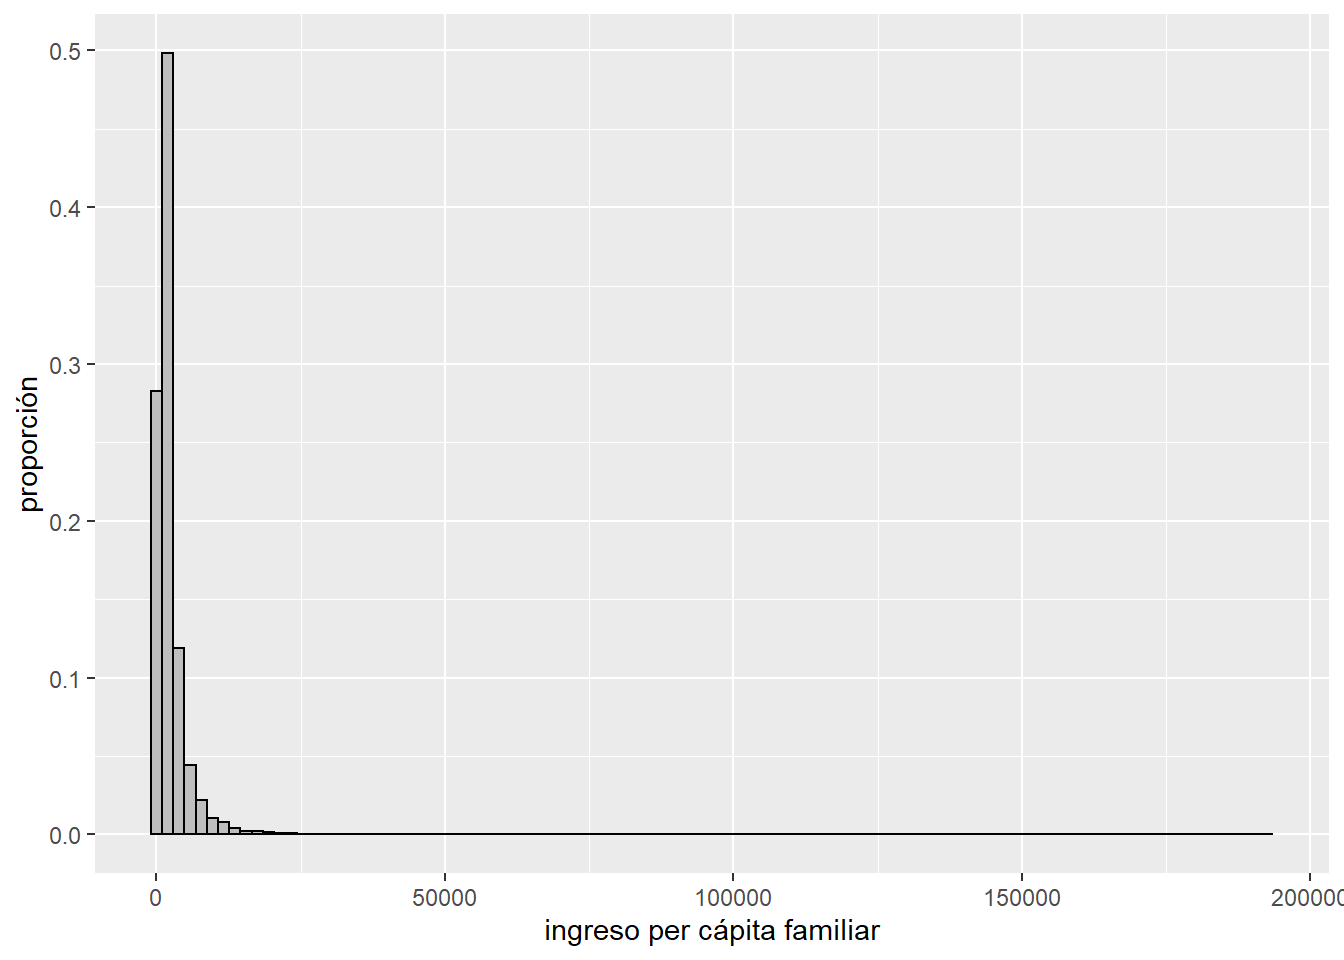
\includegraphics[width=0.8\linewidth]{_main_files/figure-latex/unnamed-chunk-16-1}

Con las líneas siguientes se filtra la base para individuos con ipcf menor a 1500 para evitar la típica distorsión generada por los valores extremos.

\begin{Shaded}
\begin{Highlighting}[]
\DocumentationTok{\#\# Figura 2.3 {-} histograma ipcf sin outliers}
\FunctionTok{ggplot}\NormalTok{(}\AttributeTok{data=}\NormalTok{mex06 }\SpecialCharTok{\%\textgreater{}\%} \FunctionTok{filter}\NormalTok{(ipcf }\SpecialCharTok{\textless{}} \DecValTok{15000}\NormalTok{), }
       \FunctionTok{aes}\NormalTok{(}\AttributeTok{x=}\NormalTok{ipcf, }\AttributeTok{weight=}\NormalTok{pondera)) }\SpecialCharTok{+} 
  \FunctionTok{geom\_histogram}\NormalTok{(}\AttributeTok{bins =} \DecValTok{100}\NormalTok{, }\FunctionTok{aes}\NormalTok{(}\AttributeTok{y =} \FunctionTok{stat}\NormalTok{(count) }\SpecialCharTok{/} \FunctionTok{sum}\NormalTok{(count)),}
                 \AttributeTok{color=}\StringTok{"black"}\NormalTok{, }\AttributeTok{fill=}\StringTok{"grey"}\NormalTok{) }\SpecialCharTok{+}
  \FunctionTok{labs}\NormalTok{(}\AttributeTok{y=}\StringTok{"proporción"}\NormalTok{, }\AttributeTok{x=}\StringTok{"ingreso per cápita familiar"}\NormalTok{)}
\end{Highlighting}
\end{Shaded}

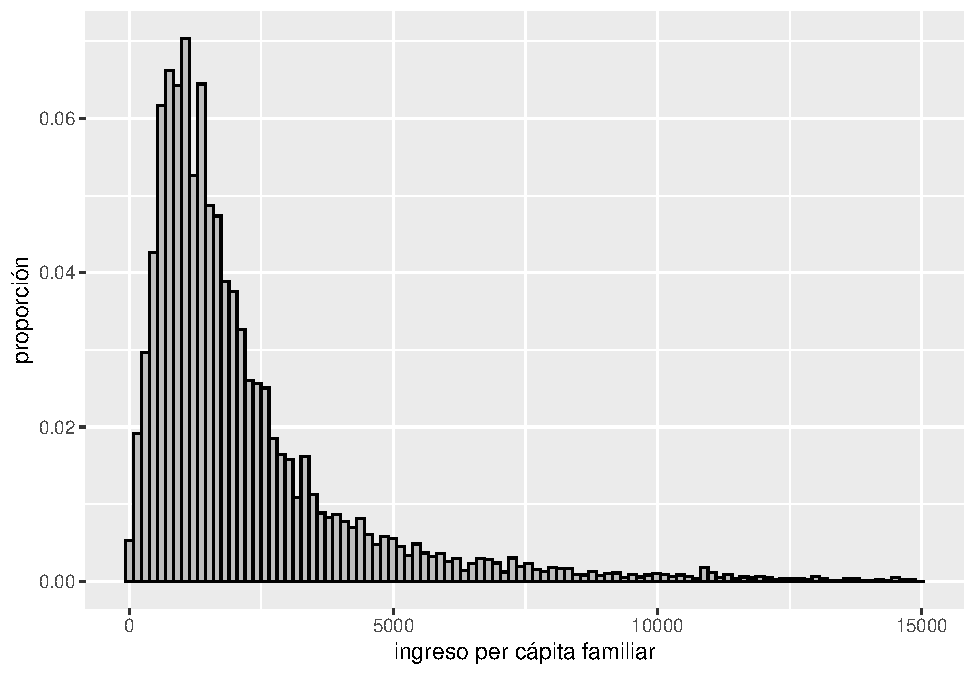
\includegraphics[width=0.8\linewidth]{_main_files/figure-latex/unnamed-chunk-17-1}

Las figuras 2.4 y 2.5 del texto pueden replicarse utilizando el bloque de código siguiente. En la primera se grafica el logaritmo de la variable ipcf, agregando simplemente la función \texttt{log()} para el eje x. En la siguiente se incrementa sucesivamente el número de barras del histograma. Para ello podríamos repetir 4 veces el gráfico cambiando solamente la cantidad de bins. Aquí optamos por presentar un solución más elegante en la que generamos los 4 gráficos a partir de un bucle que itera sobre el número de bins deseado. El lector no familiarizado con los bucles puede optar por la primera opción hasta que en los siguientes capítulos presentemos con más detalle cómo se instrumentan iteraciones mediante bucles.

\begin{Shaded}
\begin{Highlighting}[]
\DocumentationTok{\#\# Figura 2.4 {-} histograma logaritmo ipcf}
\FunctionTok{ggplot}\NormalTok{(mex06, }
       \FunctionTok{aes}\NormalTok{(}\AttributeTok{x=}\FunctionTok{log}\NormalTok{(ipcf), }\AttributeTok{weight=}\NormalTok{pondera)) }\SpecialCharTok{+} 
  \FunctionTok{geom\_histogram}\NormalTok{(}\AttributeTok{bins =} \DecValTok{100}\NormalTok{, }\FunctionTok{aes}\NormalTok{(}\AttributeTok{y =} \FunctionTok{stat}\NormalTok{(count) }\SpecialCharTok{/} \FunctionTok{sum}\NormalTok{(count)),}
                 \AttributeTok{color=}\StringTok{"black"}\NormalTok{, }\AttributeTok{fill=}\StringTok{"grey"}\NormalTok{) }\SpecialCharTok{+}
  \FunctionTok{scale\_x\_continuous}\NormalTok{(}\AttributeTok{breaks =} \FunctionTok{seq}\NormalTok{(}\DecValTok{0}\NormalTok{,}\DecValTok{15}\NormalTok{,}\DecValTok{5}\NormalTok{))}\SpecialCharTok{+}
  \FunctionTok{labs}\NormalTok{(}\AttributeTok{y=}\StringTok{"proporción"}\NormalTok{, }\AttributeTok{x=}\StringTok{"ingreso per cápita familiar"}\NormalTok{)}
\end{Highlighting}
\end{Shaded}

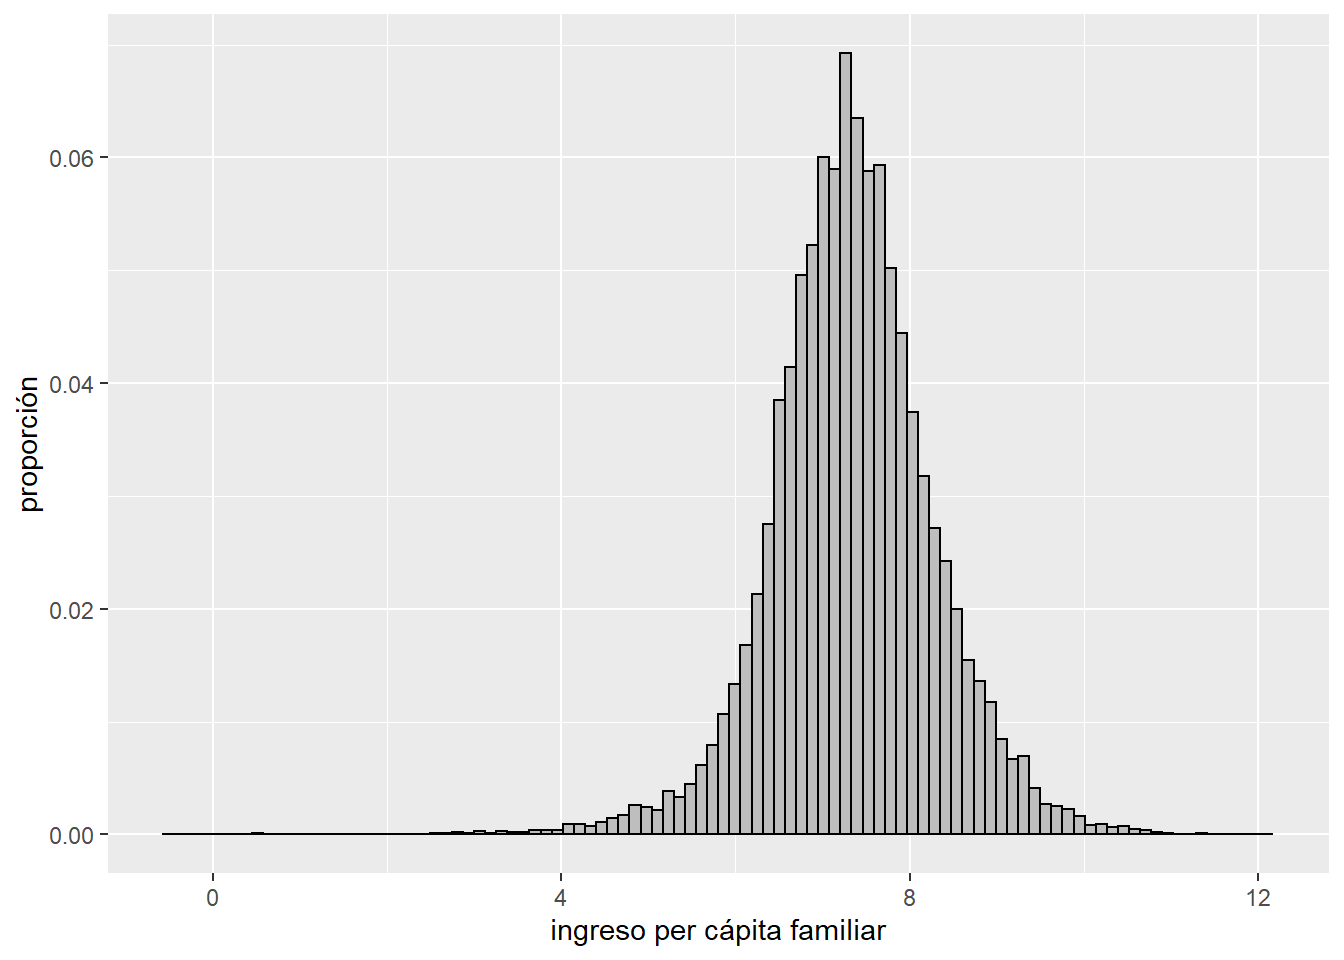
\includegraphics[width=0.8\linewidth]{_main_files/figure-latex/unnamed-chunk-18-1}

\begin{Shaded}
\begin{Highlighting}[]
\DocumentationTok{\#\# Figura 2.5 {-} histogramas con diferente cantidad de intervalos}
\NormalTok{n\_bins }\OtherTok{=} \FunctionTok{c}\NormalTok{(}\DecValTok{10}\NormalTok{,}\DecValTok{50}\NormalTok{,}\DecValTok{100}\NormalTok{,}\DecValTok{1000}\NormalTok{)}
\NormalTok{my\_graphs }\OtherTok{=} \FunctionTok{list}\NormalTok{()}

\NormalTok{i}\OtherTok{=}\DecValTok{1}
\ControlFlowTok{for}\NormalTok{ (n }\ControlFlowTok{in}\NormalTok{ n\_bins)\{}
  
\NormalTok{    my\_graphs[[i]] }\OtherTok{\textless{}{-}} \FunctionTok{ggplot}\NormalTok{(mex06, }
                           \FunctionTok{aes}\NormalTok{(}\AttributeTok{x=}\FunctionTok{log}\NormalTok{(ipcf), }\AttributeTok{weight=}\NormalTok{pondera)) }\SpecialCharTok{+} 
                   \FunctionTok{geom\_histogram}\NormalTok{(}\AttributeTok{bins =}\NormalTok{ n, }\FunctionTok{aes}\NormalTok{(}\AttributeTok{y =} \FunctionTok{stat}\NormalTok{(count) }\SpecialCharTok{/} \FunctionTok{sum}\NormalTok{(count)),}
                               \AttributeTok{color=}\StringTok{"black"}\NormalTok{, }\AttributeTok{fill=}\StringTok{"grey"}\NormalTok{) }\SpecialCharTok{+}
                   \FunctionTok{scale\_x\_continuous}\NormalTok{(}\AttributeTok{breaks =} \FunctionTok{seq}\NormalTok{(}\DecValTok{0}\NormalTok{,}\DecValTok{15}\NormalTok{,}\DecValTok{5}\NormalTok{))}\SpecialCharTok{+}
                   \FunctionTok{labs}\NormalTok{(}\AttributeTok{y=}\StringTok{"proporción"}\NormalTok{, }\AttributeTok{x=}\StringTok{"ingreso per cápita familiar"}\NormalTok{) }\SpecialCharTok{+}
                   \FunctionTok{ggtitle}\NormalTok{( n }\SpecialCharTok{\%+\%} \StringTok{" intervalos"}\NormalTok{) }\SpecialCharTok{+}
                   \FunctionTok{theme}\NormalTok{(}\AttributeTok{plot.title =} \FunctionTok{element\_text}\NormalTok{(}\AttributeTok{size =} \DecValTok{12}\NormalTok{, }\AttributeTok{hjust =} \FloatTok{0.5}\NormalTok{))}

\NormalTok{  i}\OtherTok{=}\NormalTok{i}\SpecialCharTok{+}\DecValTok{1}  
\NormalTok{\}}

\NormalTok{g1 }\OtherTok{\textless{}{-}}\NormalTok{  my\_graphs[[}\DecValTok{1}\NormalTok{]]}
\NormalTok{g2 }\OtherTok{\textless{}{-}}\NormalTok{  my\_graphs[[}\DecValTok{2}\NormalTok{]]}
\NormalTok{g3 }\OtherTok{\textless{}{-}}\NormalTok{  my\_graphs[[}\DecValTok{3}\NormalTok{]]}
\NormalTok{g4 }\OtherTok{\textless{}{-}}\NormalTok{  my\_graphs[[}\DecValTok{4}\NormalTok{]]}

\FunctionTok{library}\NormalTok{(gridExtra)}
\FunctionTok{grid.arrange}\NormalTok{(g1, g2, g3, g4, }\AttributeTok{ncol=}\DecValTok{2}\NormalTok{, }\AttributeTok{nrow=}\DecValTok{2}\NormalTok{)}
\end{Highlighting}
\end{Shaded}

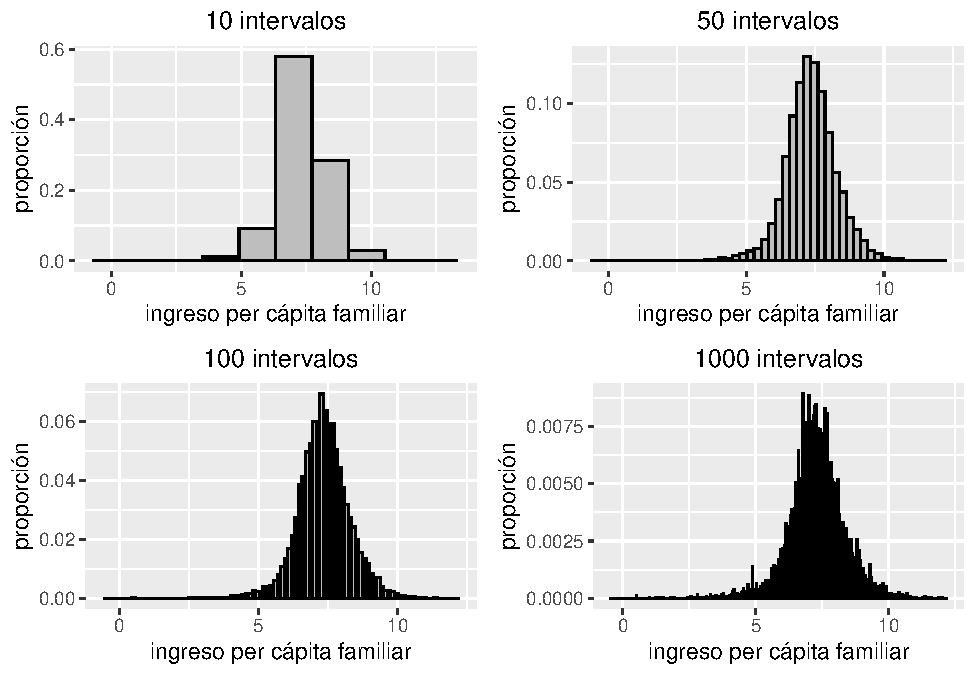
\includegraphics[width=0.9\linewidth]{_main_files/figure-latex/unnamed-chunk-19-1}

Las líneas que siguen grafican, superpuestos, los histogramas suavizados de las funciones de densidad del logaritmo del ipcf para las regiones Noroeste y Sur de México. Para este grafico, dentro de \texttt{aes()} debemos indicar no solo los ejes x e y junto con el ponderador, sino además debemos indicar que queremos que lo diferencia por grupos. Concretamente la opción \texttt{fill=factor(region)} le indica a R que el color de relleno de la curva (``fill'') estará dado por una variable de la base de datos, en este caso la variable ``región''. Dado que dicha variable en la base es del tipo numérico, empleamos \texttt{factor()} para tratarla como una categórica. Para graficar una curva de densidad el comando indicado es \texttt{geom\_density()}. Habiendo especificado estas opciones R mostrará una curva de densidad para cada región en el mismo gráfico, a partir de una misma variable (ipcf) ponderándola por el factor de expansión.

Al código se agregan algunas customizaciones mas para la densidad: \texttt{color="black"} indica que queremos bordes negros, \texttt{alpha=0.4} indica el grado de transparencia en el relleno (para que al superponer las curvas continúen siendo visibles) y \texttt{size} indica el grosor del borde simplemente. Finalmente, dado que optamos por el color de relleno para diferenciar Noroeste y Sur, controlamos estas leyendas con la opción \texttt{scale\_fill\_discrete()}. Notar que en la primer línea definimos el objeto \emph{``lp''} que contiene el valor de la línea de pobreza internacional de USD 2.5 por día por persona para México (en log), que marcamos como una línea vertical en el grafico con \texttt{geom\_vline()}.

\begin{Shaded}
\begin{Highlighting}[]
\DocumentationTok{\#\# Figura 2.7 {-} histogramas superpuestos por regiones}
\NormalTok{lp}\OtherTok{=}\FunctionTok{log}\NormalTok{(}\FloatTok{608.245}\NormalTok{)}

\FunctionTok{ggplot}\NormalTok{(mex06 }\SpecialCharTok{\%\textgreater{}\%} \FunctionTok{filter}\NormalTok{(region}\SpecialCharTok{==}\DecValTok{1} \SpecialCharTok{|}\NormalTok{ region}\SpecialCharTok{==}\DecValTok{6}\NormalTok{), }
       \FunctionTok{aes}\NormalTok{(}\AttributeTok{x=}\FunctionTok{log}\NormalTok{(ipcf), }\AttributeTok{weight=}\NormalTok{pondera, }\AttributeTok{fill=}\FunctionTok{factor}\NormalTok{(region))) }\SpecialCharTok{+} 
  \FunctionTok{geom\_density}\NormalTok{(}\AttributeTok{color=}\StringTok{"black"}\NormalTok{, }\AttributeTok{alpha =} \FloatTok{0.4}\NormalTok{, }\AttributeTok{size=}\FloatTok{0.7}\NormalTok{) }\SpecialCharTok{+}
  \FunctionTok{scale\_fill\_discrete}\NormalTok{(}\AttributeTok{name=}\StringTok{"Región"}\NormalTok{, }\AttributeTok{labels=}\FunctionTok{c}\NormalTok{(}\StringTok{"Noroeste"}\NormalTok{, }\StringTok{"Sur"}\NormalTok{)) }\SpecialCharTok{+} 
  \FunctionTok{geom\_vline}\NormalTok{(}\AttributeTok{xintercept=}\NormalTok{lp)  }\SpecialCharTok{+}
  \FunctionTok{labs}\NormalTok{(}\AttributeTok{y=}\StringTok{"densidad"}\NormalTok{, }\AttributeTok{x=}\StringTok{"logaritmo del ingreso per c?pita familiar"}\NormalTok{) }
\end{Highlighting}
\end{Shaded}

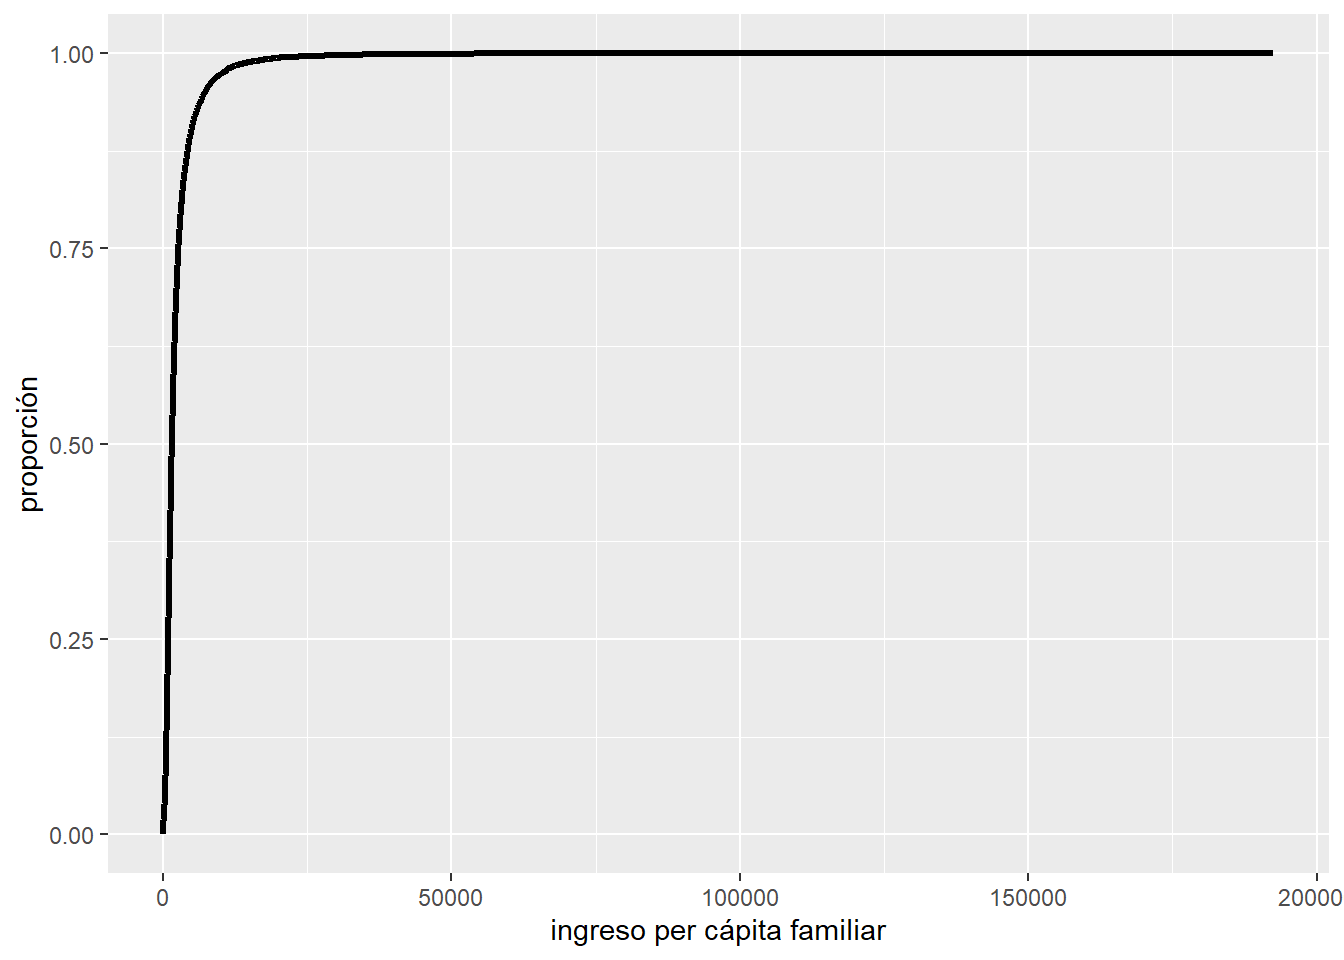
\includegraphics[width=0.8\linewidth]{_main_files/figure-latex/unnamed-chunk-20-1}

Una de las ventajas de estos histogramas suavizados es facilitar las comparaciones. Como puede verse, las dos distribuciones son claramente diferentes. La distribución del Sur está desplazada a la izquierda, lo que sugiere que en general los individuos de esa región tienen menores ingresos que en el Noroeste y por lo tanto una densidad mayor caerá por debajo de la línea de pobreza fijada en esa región.

Por último, siguiendo la figura 2.6 y 2.8, se presenta un histograma suavizado junto con una distribución normal, con la diferencia de que aquí el histograma representa la densidad y no la frecuencia relativa. En R esta opción demanda algún ajuste extra en los ejes, que aquí a los fines didácticos se omite, pero que el lector podrá replicar fácilmente siguiendo la nota al pie.\footnote{Para explorar una posible manera de plotear histogramas de frecuencia relativa o absoluta junto con un densidad suavizada el lector encontrará util la \href{https://stackoverflow.com/questions/27611438/density-curve-overlay-on-histogram-where-vertical-axis-is-frequency-aka-count}{siguiente entrada} de \emph{stackoverflow}.}

\begin{Shaded}
\begin{Highlighting}[]
\DocumentationTok{\#\# Figura 2.6/2.8 {-} histograma logaritmo ipcf suavizado}
\FunctionTok{ggplot}\NormalTok{(mex06, }
       \FunctionTok{aes}\NormalTok{(}\AttributeTok{x=}\FunctionTok{log}\NormalTok{(ipcf), }\AttributeTok{weight=}\NormalTok{pondera)) }\SpecialCharTok{+} 
  \FunctionTok{geom\_histogram}\NormalTok{(}\AttributeTok{bins =} \DecValTok{100}\NormalTok{, }\FunctionTok{aes}\NormalTok{(}\AttributeTok{y =}\NormalTok{ ..density..), }
                 \AttributeTok{color=}\StringTok{"black"}\NormalTok{, }\AttributeTok{fill=}\StringTok{"gray"}\NormalTok{)  }\SpecialCharTok{+}
  \FunctionTok{geom\_density}\NormalTok{(}\AttributeTok{kernel=}\StringTok{"gaussian"}\NormalTok{, }\AttributeTok{color=}\StringTok{"blue3"}\NormalTok{, }\AttributeTok{size=}\FloatTok{0.7}\NormalTok{) }\SpecialCharTok{+}  
  \FunctionTok{labs}\NormalTok{(}\AttributeTok{y=}\StringTok{"densidad"}\NormalTok{, }\AttributeTok{x=}\StringTok{"logaritmo del ingreso per capita familiar"}\NormalTok{)}
\end{Highlighting}
\end{Shaded}

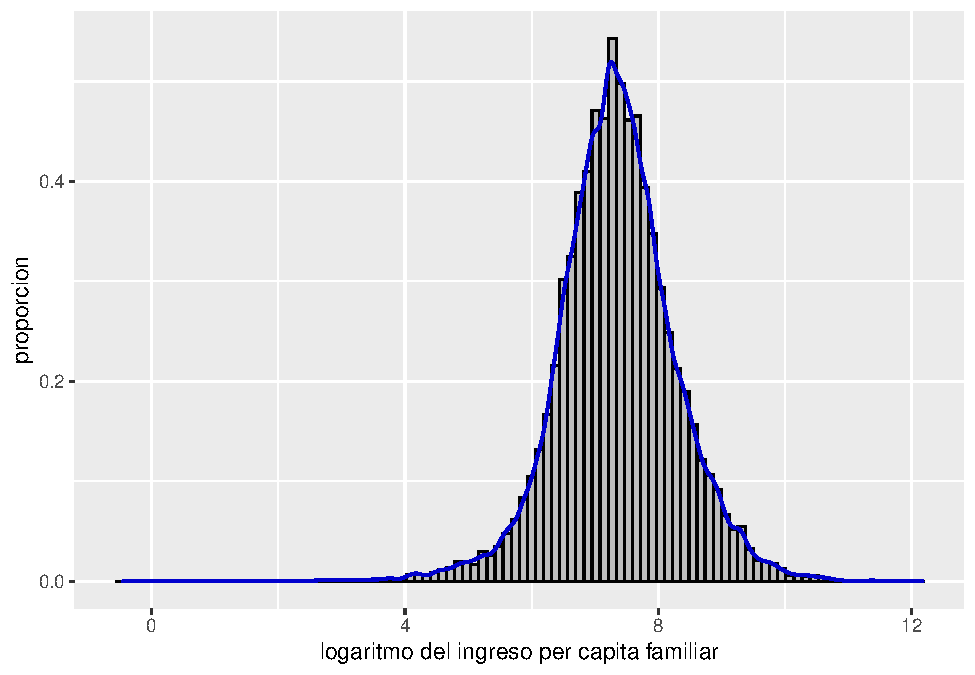
\includegraphics[width=0.8\linewidth]{_main_files/figure-latex/unnamed-chunk-21-1}

\hypertarget{funciuxf3n-de-distribuciuxf3n}{%
\section{Función de distribución}\label{funciuxf3n-de-distribuciuxf3n}}

\#\#\#- (pág. 78)

En este apartado se muestra cómo pueden graficarse las funciones de distribución presentadas en la sección 2.3.2 del cuerpo principal del capítulo. El primer paso para construir una función de distribución es ordenar (de menor a mayor) las observaciones de la encuestas, según la variable de ingreso elegida, \emph{ipcf} en nuestro caso. Esto es lo que hacemos en la primera línea. En la línea siguiente se crea la variable \emph{shrpop} para almacenar la proporción relativa acumulada de la variable \emph{pondera}, es decir el porcentaje acumulado de la población que representa cada observación junto con todas las anteriores. \emph{shrpop} tendrá entonces un valor de 100 para la última observación. Para obtener la suma acumulada expandida empleamos el comenado \texttt{cumsum()} y lo dividimos por el total de población expandido que se obtiene con \texttt{sum()}. La función de distribución presenta las variables \emph{shrpop} e \emph{ipcf} en los ejes vertical y horizontal, respectivamente, como se indica en \texttt{aes()}, y se se grafica simplemente con una línea, por lo que usamos el comando \texttt{geom\_line()}, donde solo especificamos su tamaño o grosor.

\begin{Shaded}
\begin{Highlighting}[]
\CommentTok{\#ordenar según ipcf}
\NormalTok{mex06 }\OtherTok{\textless{}{-}}\NormalTok{ mex06 }\SpecialCharTok{\%\textgreater{}\%} \FunctionTok{arrange}\NormalTok{(ipcf)}

\CommentTok{\#población acumulada ordenamiento ipcf}
\NormalTok{mex06 }\OtherTok{\textless{}{-}}\NormalTok{ mex06 }\SpecialCharTok{\%\textgreater{}\%} \FunctionTok{mutate}\NormalTok{(}\AttributeTok{shrpop=}\FunctionTok{cumsum}\NormalTok{(pondera)}\SpecialCharTok{/}\FunctionTok{sum}\NormalTok{(pondera))}

\DocumentationTok{\#\# Figura 2.9 {-} función de distribución acumulada}
\FunctionTok{ggplot}\NormalTok{(mex06, }\FunctionTok{aes}\NormalTok{(}\AttributeTok{x=}\NormalTok{ipcf, }\AttributeTok{y=}\NormalTok{shrpop))}\SpecialCharTok{+}
  \FunctionTok{geom\_line}\NormalTok{(}\AttributeTok{size=}\FloatTok{1.2}\NormalTok{) }\SpecialCharTok{+}
  \FunctionTok{labs}\NormalTok{(}\AttributeTok{y=}\StringTok{"proporción"}\NormalTok{, }\AttributeTok{x=}\StringTok{"ingreso per cápita familiar"}\NormalTok{)}
\end{Highlighting}
\end{Shaded}

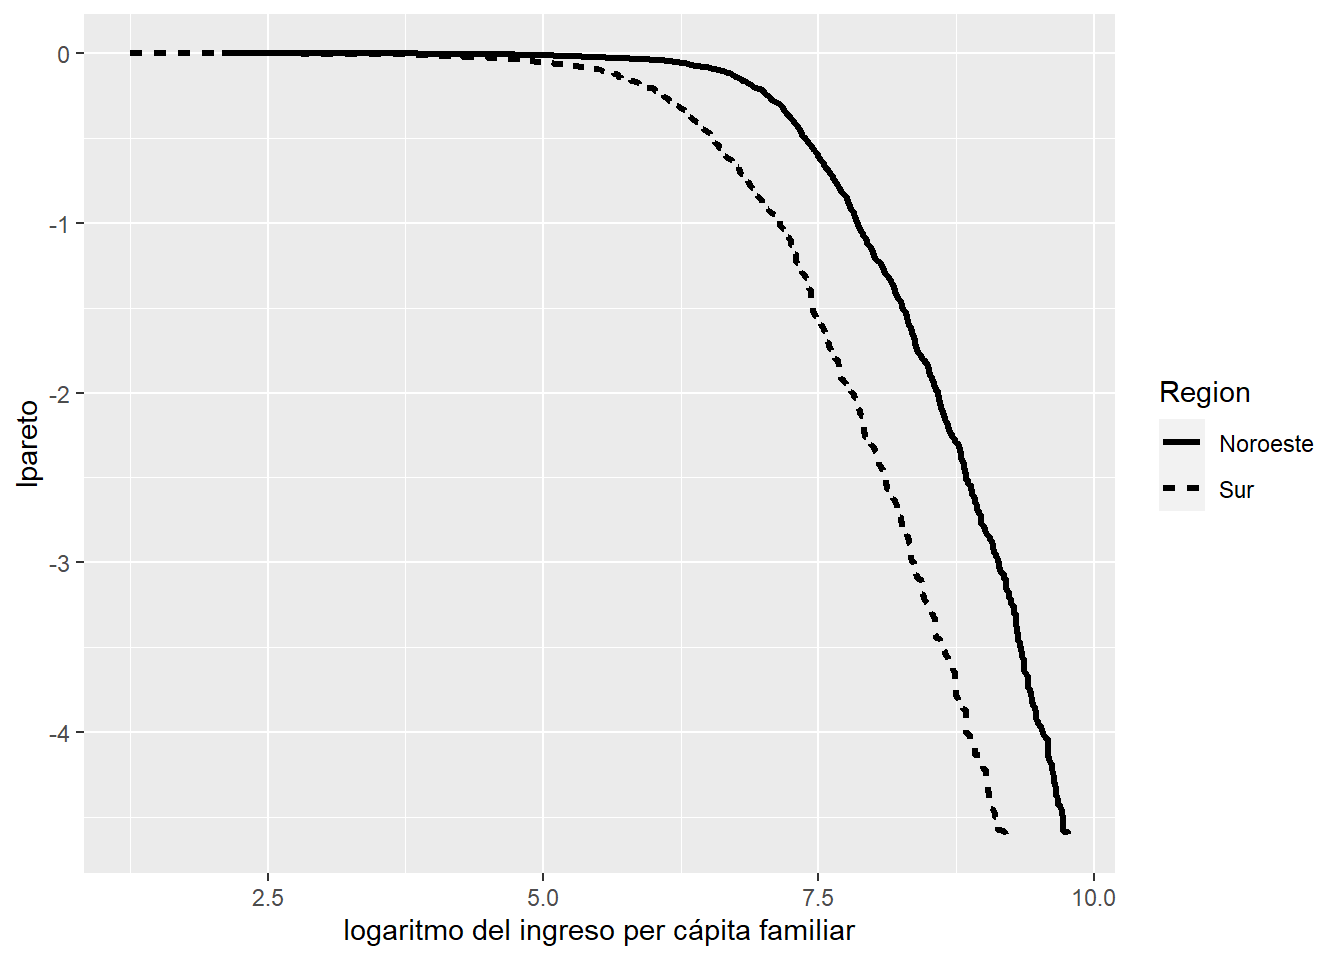
\includegraphics[width=0.8\linewidth]{_main_files/figure-latex/unnamed-chunk-22-1}

Nuevamente, la cola superior larga de la distribución vuelve al gráfico poco útil. Para
aliviar este problema las alternativas son o bien truncar los valores superiores del ingreso, o
trabajar en logaritmos. La figura 2.10 muestra ambas alternativas. Para la primera, en vez de establacer una valor arbitrario a mano, calculamos el ingreso del percentil 95 y en base a este umbral filtramos las observaciones.

\begin{Shaded}
\begin{Highlighting}[]
\DocumentationTok{\#\# Figura 2.10 función de distribución acumulada sin outliers}
\NormalTok{p95 }\OtherTok{=} \FunctionTok{wtd.quantile}\NormalTok{(mex06}\SpecialCharTok{$}\NormalTok{ipcf, }\AttributeTok{probs=}\FloatTok{0.95}\NormalTok{, }\AttributeTok{w=}\NormalTok{mex06}\SpecialCharTok{$}\NormalTok{pondera)}
\NormalTok{trunca  }\OtherTok{\textless{}{-}} \FunctionTok{ggplot}\NormalTok{(mex06 }\SpecialCharTok{\%\textgreater{}\%} \FunctionTok{filter}\NormalTok{(ipcf}\SpecialCharTok{\textless{}}\NormalTok{p95), }
                \FunctionTok{aes}\NormalTok{(}\AttributeTok{x=}\NormalTok{ipcf, }\AttributeTok{y=}\NormalTok{shrpop))}\SpecialCharTok{+}
           \FunctionTok{geom\_line}\NormalTok{(}\AttributeTok{size=}\FloatTok{1.2}\NormalTok{) }\SpecialCharTok{+}
           \FunctionTok{ggtitle}\NormalTok{(}\StringTok{"Ignora 5\% mas rico"}\NormalTok{)}\SpecialCharTok{+}
           \FunctionTok{labs}\NormalTok{(}\AttributeTok{y=}\StringTok{"proporción"}\NormalTok{, }\AttributeTok{x=}\StringTok{"ingreso per cápita familiar"}\NormalTok{) }

\NormalTok{logipcf }\OtherTok{\textless{}{-}} \FunctionTok{ggplot}\NormalTok{(mex06, }
                  \FunctionTok{aes}\NormalTok{(}\AttributeTok{x=}\FunctionTok{log}\NormalTok{(ipcf), }\AttributeTok{y=}\NormalTok{shrpop))}\SpecialCharTok{+}
           \FunctionTok{geom\_line}\NormalTok{(}\AttributeTok{size=}\FloatTok{1.2}\NormalTok{) }\SpecialCharTok{+}
           \FunctionTok{ggtitle}\NormalTok{(}\StringTok{"Toda la población"}\NormalTok{) }\SpecialCharTok{+}
           \FunctionTok{labs}\NormalTok{(}\AttributeTok{y=}\StringTok{"proporción"}\NormalTok{, }\AttributeTok{x=}\StringTok{"ingreso per cápita familiar"}\NormalTok{)  }


\FunctionTok{grid.arrange}\NormalTok{(trunca, logipcf, }\AttributeTok{ncol=}\DecValTok{2}\NormalTok{)}
\end{Highlighting}
\end{Shaded}

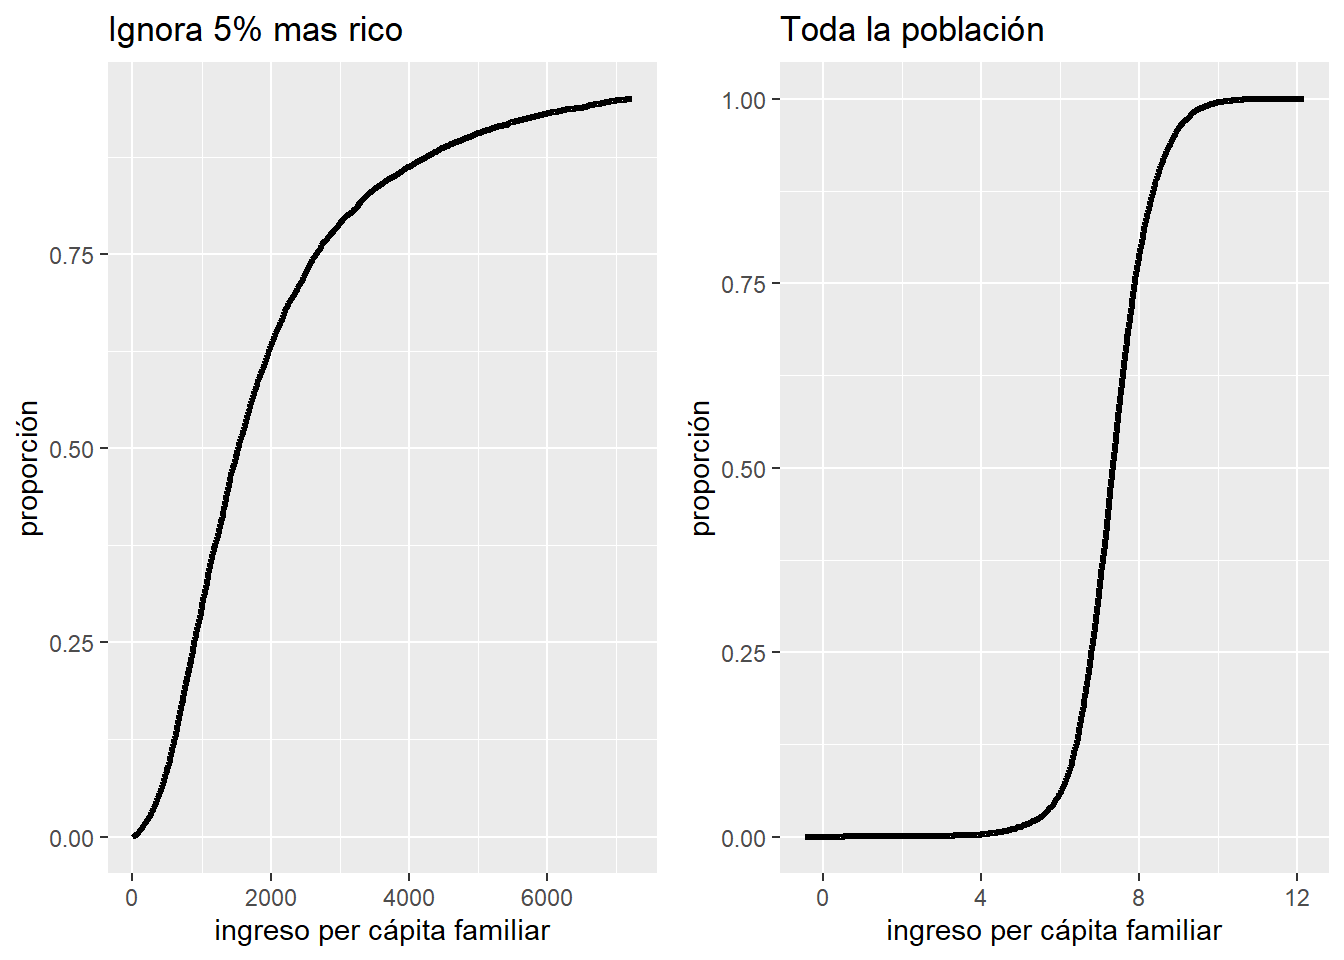
\includegraphics[width=0.8\linewidth]{_main_files/figure-latex/unnamed-chunk-23-1}

Se deja como ejercicio para el lector elaborar las otras funciones de distribución presentadas en la sección 2.3.2. Por su parte, la curva de Pen (ver figuras 2.12 y 2.13) se construye igual que la función de distribución pero se grafica invirtiendo los ejes.

\hypertarget{pareto}{%
\section{Pareto}\label{pareto}}

\#\#\#- (pág. 78)

En esta sección se muestra cómo replicar la figura 2.14 del texto, que muestra los diagramas de Pareto para las regiones Noroeste y Sur de México. El procedimiento es muy similar al caso de la función de distribución ya que en esencia representan lo mismo, de forma distinta. El gráfico de Pareto muestra para cada valor del ingreso x el porcentaje de la población que recibe ingresos superiores a ese valor x, en una escala doble logarítmica. El cambio de escala genera una suerte de zoom óptico sobre los estratos de mayores ingresos, permitiendo un examen más detallado de esa parte de la distribución.

Para graficarlo seguimos los pasos anteriores, pero ahora ordenamos a la población por ingreso dentro de cada región y ya no considerando el total país. Para ello agrupamos las observaciones por región con \texttt{group\_by()} previo a calcular el share acumulado, de forma tal que este cálculo se haga solo entre individuos de una misma región. En la siguiente línea se genera la variable \emph{lpareto} a partir de la variable \emph{shrpop}, siguiendo la explicación de la sección 2.3.4 del texto. Finalmente se grafica filtrando la base para las regiones de interés y, siguiendo la misma lógica empleada en el grafico de densidad superpuesta, indicamos dentro de \texttt{aes()} la opción \texttt{linetype} para lograr un tipo de línea diferente que distinga a cada región. Notar que aquí también empleamos \texttt{factor()} para tratar esta variable categórica. Por último, con \texttt{scale\_linetype()} customizamos las leyendas.

\begin{Shaded}
\begin{Highlighting}[]
\CommentTok{\#población acumulada por región}
\NormalTok{mex06 }\OtherTok{\textless{}{-}}\NormalTok{ mex06 }\SpecialCharTok{\%\textgreater{}\%} \FunctionTok{group\_by}\NormalTok{(region) }\SpecialCharTok{\%\textgreater{}\%} \FunctionTok{mutate}\NormalTok{(}\AttributeTok{shrpop=}\FunctionTok{cumsum}\NormalTok{(pondera)}\SpecialCharTok{/}\FunctionTok{sum}\NormalTok{(pondera)) }

\NormalTok{mex06 }\OtherTok{\textless{}{-}}\NormalTok{ mex06 }\SpecialCharTok{\%\textgreater{}\%} \FunctionTok{mutate}\NormalTok{(}\AttributeTok{lpareto=}\FunctionTok{log}\NormalTok{(}\DecValTok{1}\SpecialCharTok{{-}}\NormalTok{shrpop)) }

\DocumentationTok{\#\# Figura 2.14 {-} Diagrama de Pareto}
\FunctionTok{ggplot}\NormalTok{(mex06 }\SpecialCharTok{\%\textgreater{}\%} \FunctionTok{filter}\NormalTok{(region}\SpecialCharTok{==}\DecValTok{1} \SpecialCharTok{|}\NormalTok{ region}\SpecialCharTok{==}\DecValTok{6}\NormalTok{), }
       \FunctionTok{aes}\NormalTok{(}\AttributeTok{x=}\FunctionTok{log}\NormalTok{(ipcf), }\AttributeTok{y=}\NormalTok{lpareto, }\AttributeTok{weight=}\NormalTok{pondera, }\AttributeTok{linetype=}\FunctionTok{factor}\NormalTok{(region))) }\SpecialCharTok{+} 
  \FunctionTok{geom\_line}\NormalTok{(}\AttributeTok{size=}\FloatTok{1.2}\NormalTok{) }\SpecialCharTok{+}
  \FunctionTok{scale\_linetype}\NormalTok{(}\AttributeTok{name=}\StringTok{"Región"}\NormalTok{, }\AttributeTok{labels=}\FunctionTok{c}\NormalTok{(}\StringTok{"Noroeste"}\NormalTok{, }\StringTok{"Sur"}\NormalTok{)) }\SpecialCharTok{+} 
  \FunctionTok{labs}\NormalTok{(}\AttributeTok{x=}\StringTok{"logaritmo del ingreso per cápita familiar"}\NormalTok{)}
\end{Highlighting}
\end{Shaded}

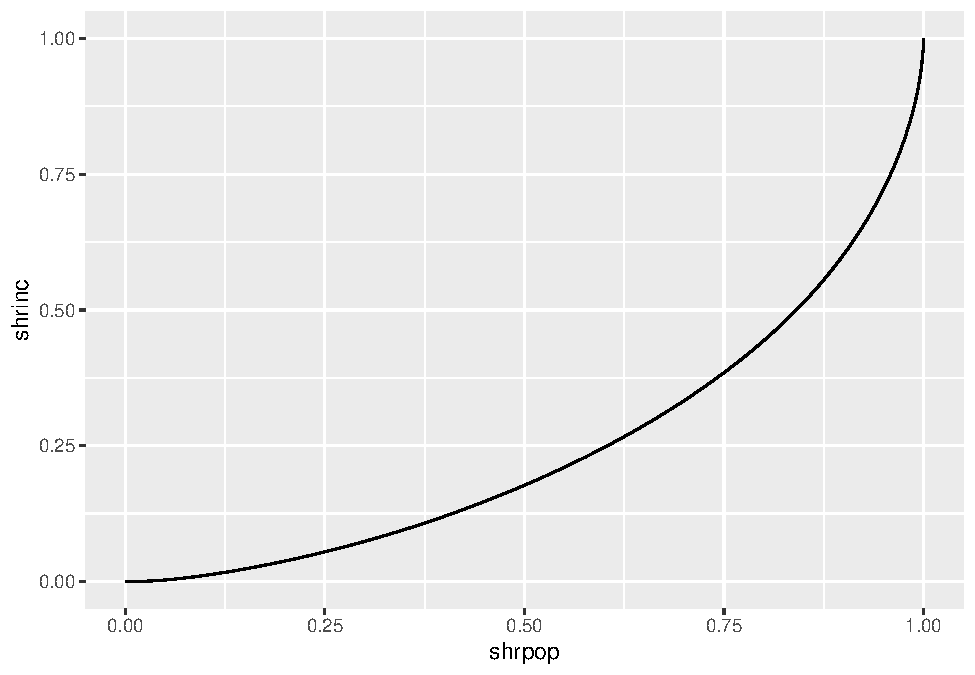
\includegraphics[width=0.8\linewidth]{_main_files/figure-latex/unnamed-chunk-24-1}

Las líneas siguientes repiten el ejercicio pero dejando de lado al 1\% más rico de la poblacion en cada región. Aquí en vez de filtrar en base al valor de ingresos, lo hacemos en base al porcentaje acumulado, como alternativa al caso anterior.

\begin{Shaded}
\begin{Highlighting}[]
\NormalTok{cutoff}\OtherTok{=}\FloatTok{0.99}

\FunctionTok{ggplot}\NormalTok{(mex06 }\SpecialCharTok{\%\textgreater{}\%} \FunctionTok{filter}\NormalTok{((region}\SpecialCharTok{==}\DecValTok{1} \SpecialCharTok{|}\NormalTok{ region}\SpecialCharTok{==}\DecValTok{6}\NormalTok{) }\SpecialCharTok{\&}\NormalTok{ (shrpop}\SpecialCharTok{\textless{}=}\NormalTok{cutoff)),}
       \FunctionTok{aes}\NormalTok{(}\AttributeTok{x=}\FunctionTok{log}\NormalTok{(ipcf), }\AttributeTok{y=}\NormalTok{lpareto, }\AttributeTok{weight=}\NormalTok{pondera, }\AttributeTok{linetype=}\FunctionTok{factor}\NormalTok{(region))) }\SpecialCharTok{+} 
  \FunctionTok{geom\_line}\NormalTok{(}\AttributeTok{size=}\FloatTok{1.2}\NormalTok{) }\SpecialCharTok{+}
  \FunctionTok{scale\_linetype}\NormalTok{(}\AttributeTok{name=}\StringTok{"Región"}\NormalTok{, }\AttributeTok{labels=}\FunctionTok{c}\NormalTok{(}\StringTok{"Noroeste"}\NormalTok{, }\StringTok{"Sur"}\NormalTok{)) }\SpecialCharTok{+} 
  \FunctionTok{labs}\NormalTok{(}\AttributeTok{x=}\StringTok{"logaritmo del ingreso per cápita familiar"}\NormalTok{)}
\end{Highlighting}
\end{Shaded}

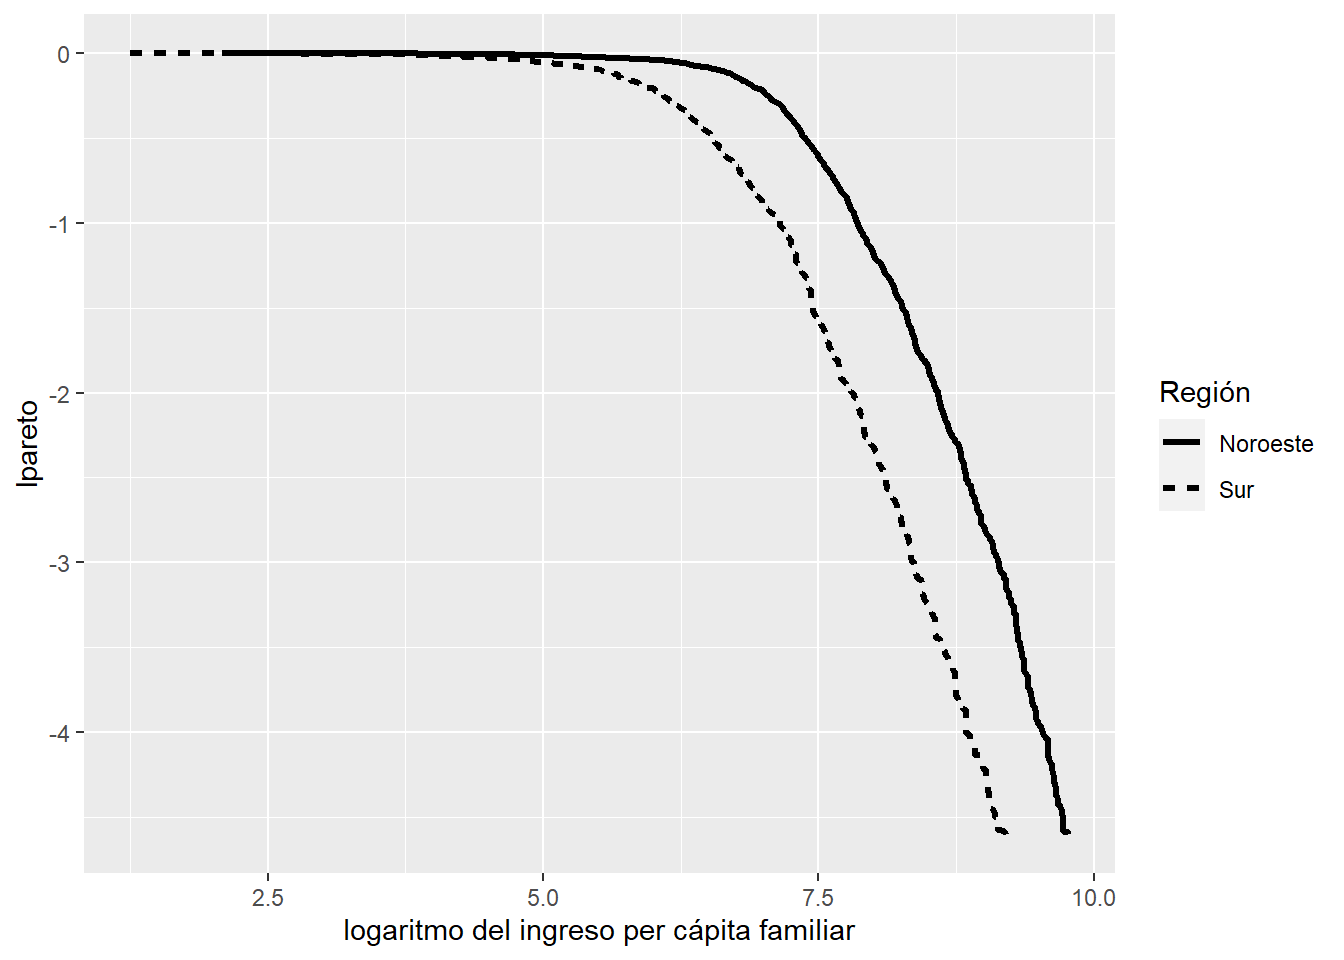
\includegraphics[width=0.8\linewidth]{_main_files/figure-latex/unnamed-chunk-25-1}

\hypertarget{box-plot}{%
\section{Box-plot}\label{box-plot}}

\#\#\#- (pág. 79)

Aquí se muestra cómo elaborar diagramas de caja o box-plot como los presentados en la sección 2.3.5 del texto. En este caso haremos una excepción y presentamos primero una alternativa más directa a \texttt{ggplot} que permite manejar facilmente los outliers, a partir de la libreria base de R. El grafico 2.17 retoma la sintaxís habitual de ggplot para costruir un box-plot para cada región. El lector podrá entender rapidamente el código en ambos casos. En el gráfico conjunto, al igual que antes, diferenciamos a las regiones por el color de relleno en cada box, especificando la opción \texttt{fill} y empleamos \texttt{factor()} para tratar a la variable como categórica. Dado que en este caso la vaiable irá en el eje x diferenciando a las regiones, le agregamos las labels correspondientes con la función \texttt{scale\_x\_discrete()}. La opción \texttt{alpha=} la utilizamos para darle transparencia al relleno y \texttt{legend.position=none} para omitir la leyenda de cada color.

\begin{Shaded}
\begin{Highlighting}[]
\CommentTok{\#Una opción mas directa fuera de ggplot}

\DocumentationTok{\#\# Figura 2.15 {-} Box Plot excluyendo outliers}
\FunctionTok{boxplot}\NormalTok{(mex06}\SpecialCharTok{$}\NormalTok{ipcf, }\AttributeTok{outline =} \ConstantTok{FALSE}\NormalTok{)}
\end{Highlighting}
\end{Shaded}

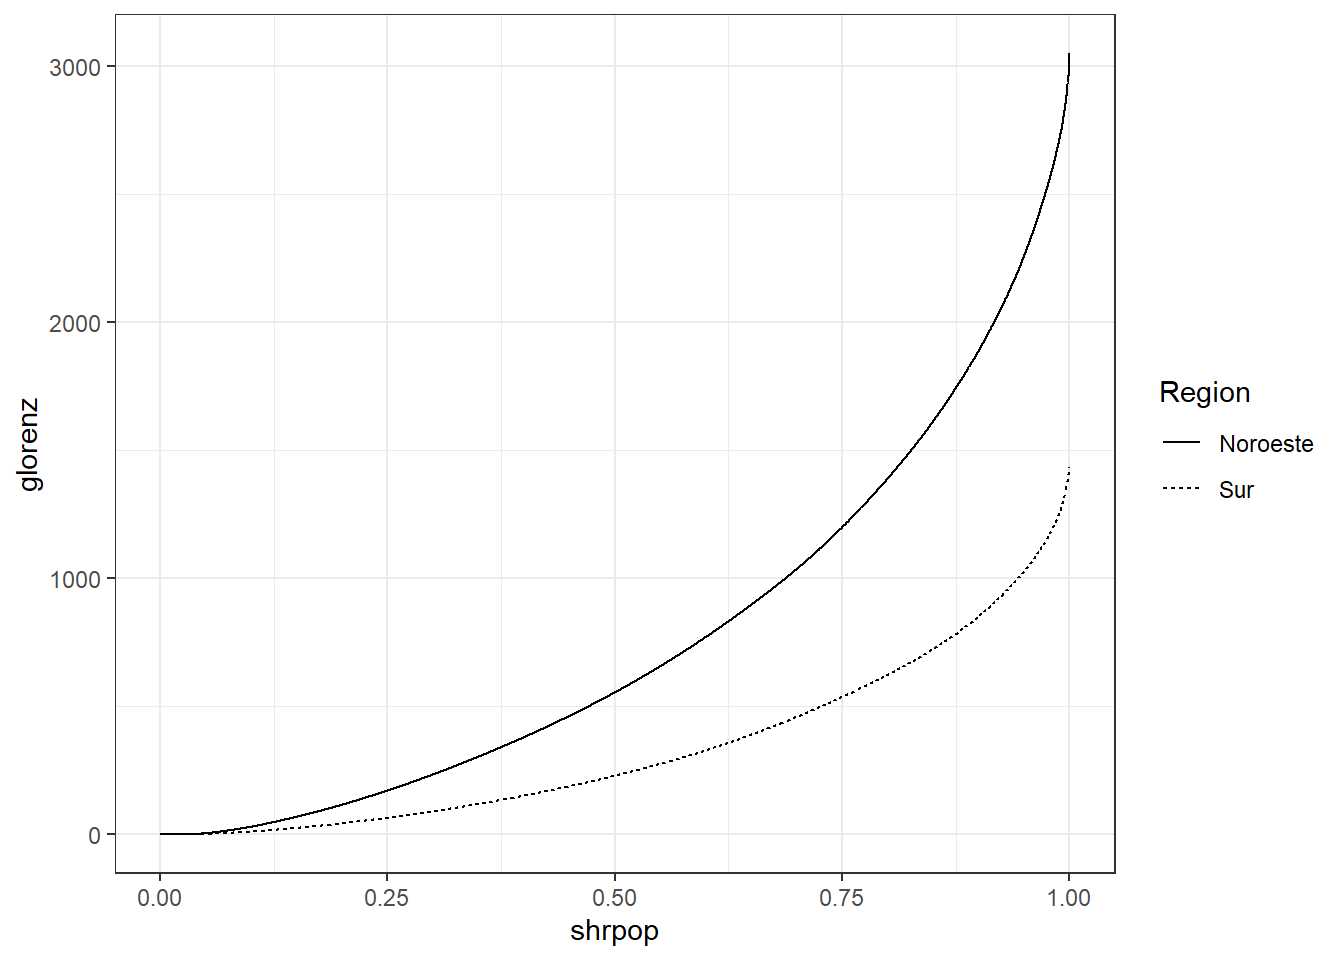
\includegraphics[width=0.8\linewidth]{_main_files/figure-latex/unnamed-chunk-26-1}

\begin{Shaded}
\begin{Highlighting}[]
\DocumentationTok{\#\# Figura 2.16 {-} Box Plot en log con outliers}
\FunctionTok{boxplot}\NormalTok{(}\FunctionTok{log}\NormalTok{(mex06}\SpecialCharTok{$}\NormalTok{ipcf), }\AttributeTok{outline =} \ConstantTok{TRUE}\NormalTok{)}
\end{Highlighting}
\end{Shaded}

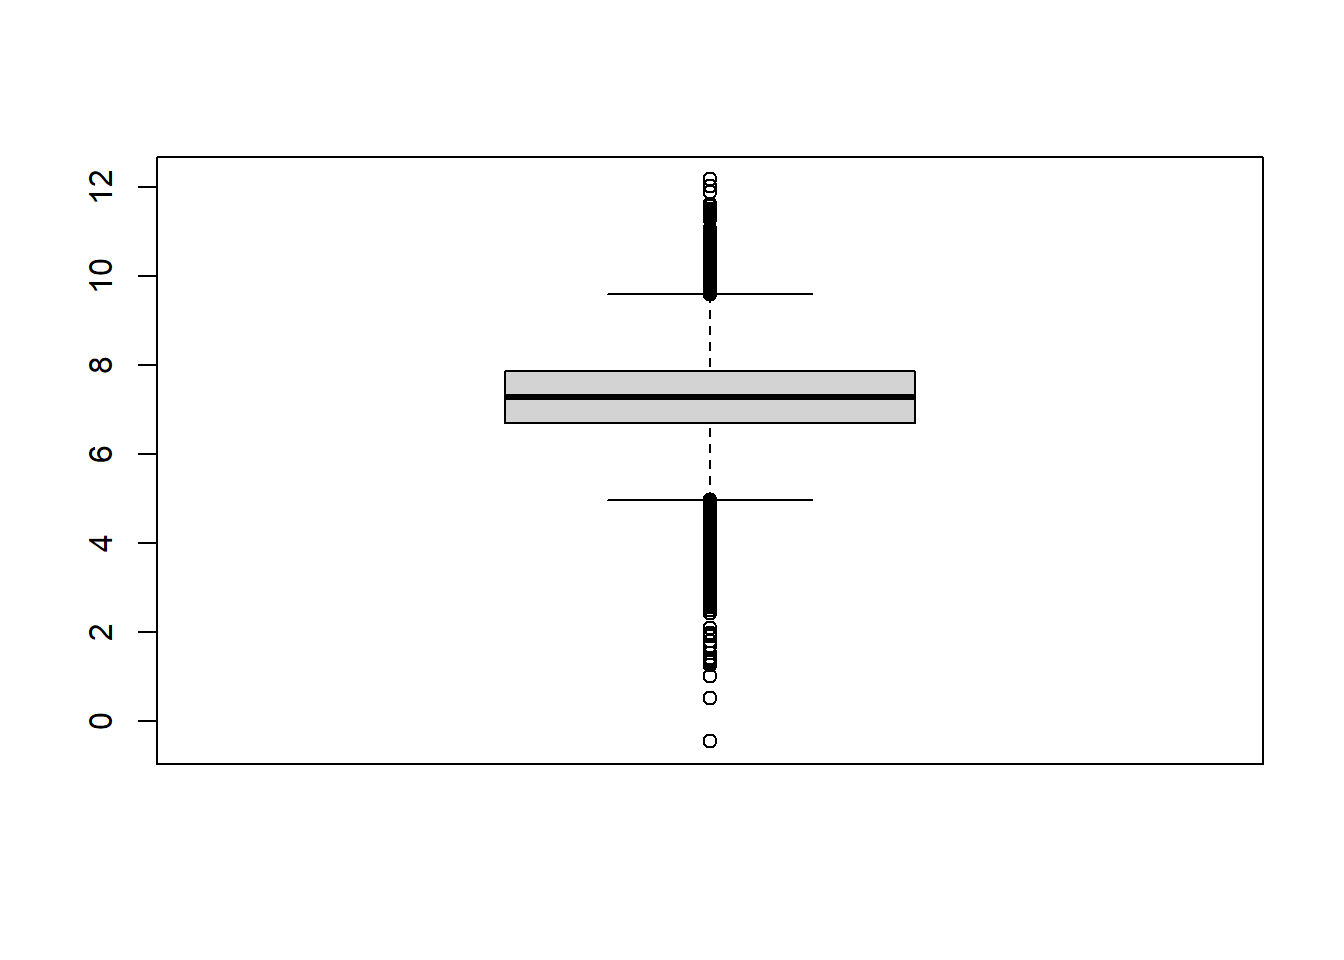
\includegraphics[width=0.8\linewidth]{_main_files/figure-latex/unnamed-chunk-26-2}

\begin{Shaded}
\begin{Highlighting}[]
\DocumentationTok{\#\# Figura 2.17  {-} Box Plot en log por regiones con outliers}
\FunctionTok{ggplot}\NormalTok{(mex06 }\SpecialCharTok{\%\textgreater{}\%} \FunctionTok{filter}\NormalTok{(region}\SpecialCharTok{==}\DecValTok{1} \SpecialCharTok{|}\NormalTok{ region}\SpecialCharTok{==}\DecValTok{6}\NormalTok{), }
       \FunctionTok{aes}\NormalTok{(}\AttributeTok{x=}\FunctionTok{factor}\NormalTok{(region), }\AttributeTok{y=}\FunctionTok{log}\NormalTok{(ipcf), }\AttributeTok{weight=}\NormalTok{pondera, }\AttributeTok{fill=}\FunctionTok{factor}\NormalTok{(region))) }\SpecialCharTok{+} 
  \FunctionTok{geom\_boxplot}\NormalTok{(}\AttributeTok{alpha=}\FloatTok{0.4}\NormalTok{) }\SpecialCharTok{+}
  \FunctionTok{theme}\NormalTok{(}\AttributeTok{legend.position=}\StringTok{"none"}\NormalTok{) }\SpecialCharTok{+} 
  \FunctionTok{scale\_x\_discrete}\NormalTok{(}\AttributeTok{labels =} \FunctionTok{c}\NormalTok{(}\StringTok{"Noroeste"}\NormalTok{,}\StringTok{"Sur"}\NormalTok{)) }\SpecialCharTok{+}
  \FunctionTok{labs}\NormalTok{(}\AttributeTok{x=}\StringTok{"Región"}\NormalTok{, }\AttributeTok{y =}\StringTok{"log ipcf"}\NormalTok{)}
\end{Highlighting}
\end{Shaded}

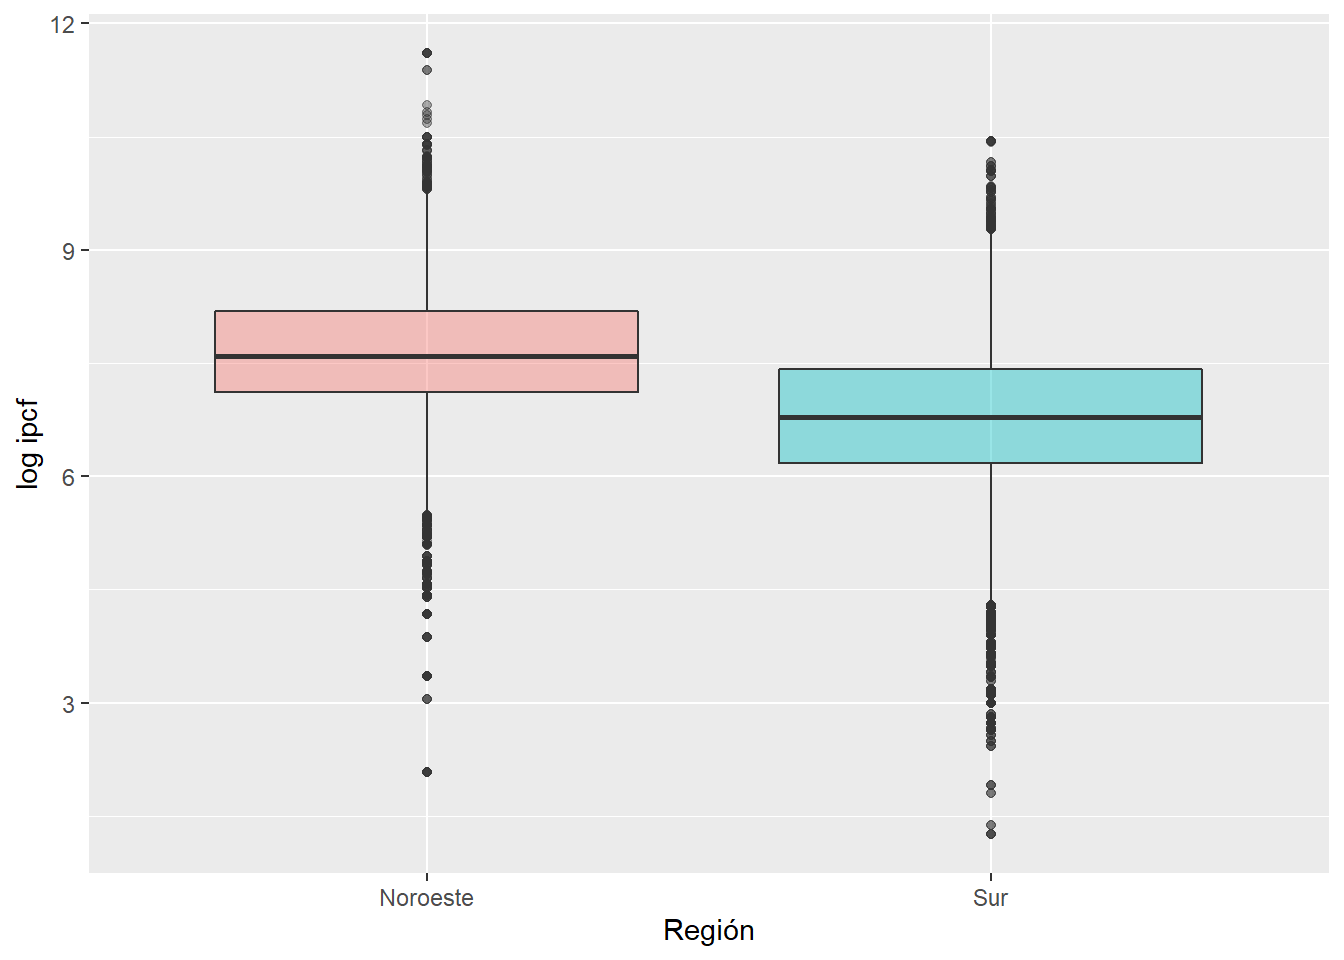
\includegraphics[width=0.8\linewidth]{_main_files/figure-latex/unnamed-chunk-26-3}

\hypertarget{curva-de-lorenz}{%
\section{Curva de Lorenz}\label{curva-de-lorenz}}

\#\#\#- (pág. 80)

En este apartado se muestra cómo pueden construirse las curvas de Lorenz introducidas en la sección 2.3.6 del capítulo. El primer paso consiste en ordenar a los individuos de menor a mayor según su ingreso, en nuestro caso contenido en la variable ipcf. Para ellos aplicamos la función \texttt{arrange()}. Notar que previo a esto se aplica la función \texttt{ungroup()}, lo cual es siempre recomendable cuando en la misma base ya se había realizado una agrupación, para de alguna forma ``resetear'' ese agrupamiento previo. Las líneas siguientes generan la variable \emph{shrpop} de la misma forma en la que fue generada más arriba, estimando la proporción de la población que se acumula hasta cada observación de la encuesta. La diferencia es que ahora también generaremos una variable \emph{shrinc} que contiene la proporción del ingreso que se acumula hasta cada observación y que se estima expandiendo el ingreso por el ponderador, es decir multiplicando ambas columnas, como puede verse en el código.

La curva de Lorenz nos muestra qué porcentaje de la población acumula un dado porcentaje del ingreso total. Para visualizarlo indicamos entonces los ejes respectivos para \emph{shrpop} y \emph{shrinc} y luego aplicamos un gráfico de línea con \texttt{geom\_line()}.

\begin{Shaded}
\begin{Highlighting}[]
\CommentTok{\#ordenar según ipcf}
\NormalTok{mex06 }\OtherTok{\textless{}{-}}\NormalTok{ mex06 }\SpecialCharTok{\%\textgreater{}\%} \FunctionTok{ungroup}\NormalTok{() }\SpecialCharTok{\%\textgreater{}\%} \FunctionTok{arrange}\NormalTok{(ipcf)}

\CommentTok{\#población e ingreso acumulado}
\NormalTok{mex06 }\OtherTok{\textless{}{-}}\NormalTok{ mex06 }\SpecialCharTok{\%\textgreater{}\%} \FunctionTok{mutate}\NormalTok{(}\AttributeTok{shrpop=}\FunctionTok{cumsum}\NormalTok{(pondera)}\SpecialCharTok{/}\FunctionTok{sum}\NormalTok{(pondera),}
                          \AttributeTok{shrinc=}\FunctionTok{cumsum}\NormalTok{(ipcf}\SpecialCharTok{*}\NormalTok{pondera)}\SpecialCharTok{/}\FunctionTok{sum}\NormalTok{(ipcf}\SpecialCharTok{*}\NormalTok{pondera)) }

\DocumentationTok{\#\# Figura 2.18 {-} curva de Lorenz }
\FunctionTok{ggplot}\NormalTok{(mex06, }\FunctionTok{aes}\NormalTok{(}\AttributeTok{x=}\NormalTok{shrpop, }\AttributeTok{y=}\NormalTok{shrinc)) }\SpecialCharTok{+}
  \FunctionTok{geom\_line}\NormalTok{()}
\end{Highlighting}
\end{Shaded}

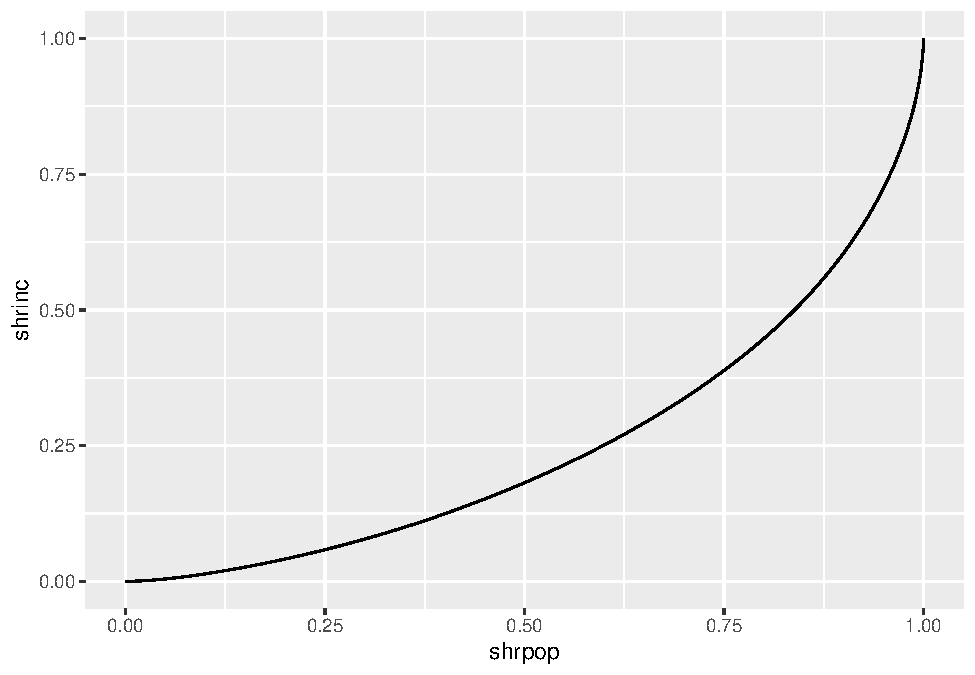
\includegraphics[width=0.8\linewidth]{_main_files/figure-latex/unnamed-chunk-27-1}

En las líneas siguientes se comparan las curvas de Lorenz para dos regiones de México. El código sigue los mismos pasos que antes pero ahora los cálculos de población e ingreso acumulado se realizan por región, agregando un \texttt{group\_by()}. En el gráfico filtramos las regiones en cuestión y las diferenciamos con distintos tipos de líneas con la opción \emph{linetype}, al igual que antes. Con \texttt{theme\_bw()}, elegimos una temática diferente para modificar un poco el aspecto visual del gráfico.

\begin{Shaded}
\begin{Highlighting}[]
\CommentTok{\#ordenar según ipcf + región y acumular por región}
\NormalTok{mex06 }\OtherTok{\textless{}{-}}\NormalTok{ mex06 }\SpecialCharTok{\%\textgreater{}\%} \FunctionTok{arrange}\NormalTok{(region, ipcf) }\SpecialCharTok{\%\textgreater{}\%} 
                   \FunctionTok{group\_by}\NormalTok{(region) }\SpecialCharTok{\%\textgreater{}\%} 
                   \FunctionTok{mutate}\NormalTok{(}\AttributeTok{shrpop=}\FunctionTok{cumsum}\NormalTok{(pondera)}\SpecialCharTok{/}\FunctionTok{sum}\NormalTok{(pondera),}
                          \AttributeTok{shrinc=}\FunctionTok{cumsum}\NormalTok{(ipcf}\SpecialCharTok{*}\NormalTok{pondera)}\SpecialCharTok{/}\FunctionTok{sum}\NormalTok{(ipcf}\SpecialCharTok{*}\NormalTok{pondera)) }

\DocumentationTok{\#\# Figura 2.19 {-} curva de lorenz por regiones}
\FunctionTok{ggplot}\NormalTok{(mex06 }\SpecialCharTok{\%\textgreater{}\%} \FunctionTok{filter}\NormalTok{(region}\SpecialCharTok{==}\DecValTok{1} \SpecialCharTok{|}\NormalTok{ region}\SpecialCharTok{==}\DecValTok{6}\NormalTok{),}
       \FunctionTok{aes}\NormalTok{(}\AttributeTok{x=}\NormalTok{shrpop, }\AttributeTok{y=}\NormalTok{shrinc, }\AttributeTok{linetype=}\FunctionTok{factor}\NormalTok{(region))) }\SpecialCharTok{+}
  \FunctionTok{geom\_line}\NormalTok{() }\SpecialCharTok{+}
  \FunctionTok{scale\_linetype}\NormalTok{(}\AttributeTok{name=}\StringTok{"Region"}\NormalTok{, }\AttributeTok{labels=}\FunctionTok{c}\NormalTok{(}\StringTok{"Noroeste"}\NormalTok{, }\StringTok{"Sur"}\NormalTok{)) }\SpecialCharTok{+}
  \FunctionTok{theme\_bw}\NormalTok{()}
\end{Highlighting}
\end{Shaded}

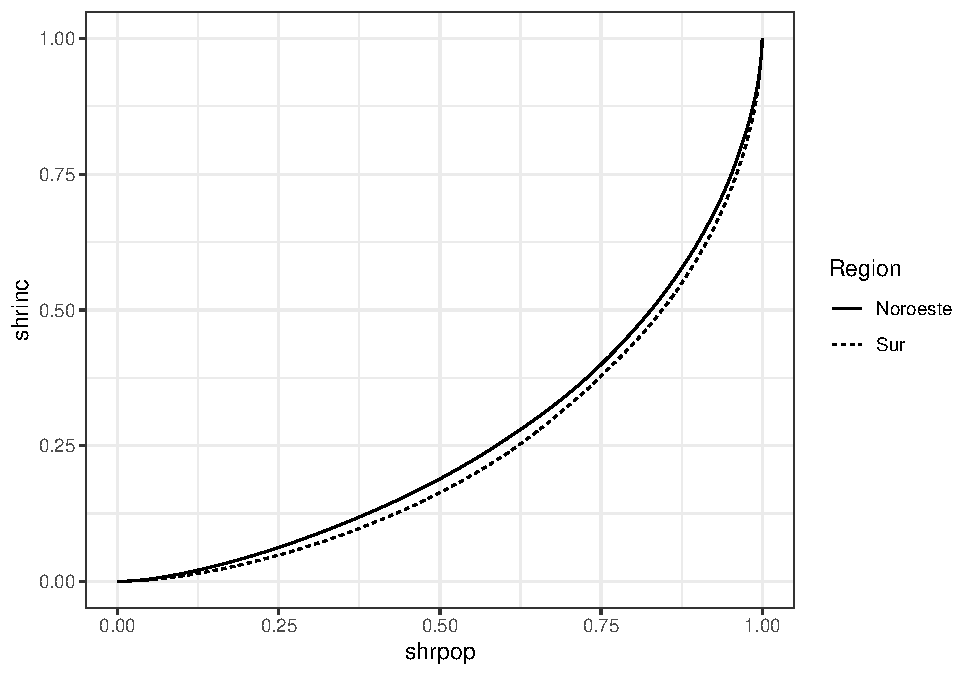
\includegraphics[width=0.8\linewidth]{_main_files/figure-latex/unnamed-chunk-28-1}

\hypertarget{curva-generalizada-de-lorenz}{%
\section{Curva Generalizada de Lorenz}\label{curva-generalizada-de-lorenz}}

\#\#\#- (pág. 81)

La curva generalizada de Lorenz se construye a partir de la curva de Lorenz pero multiplicando su eje vertical por el ingreso promedio (ver sección 2.3.6 en el cuerpo del capítulo). Las líneas de código no se modifican respecto de las utilizadas para estimar la curva de Lorenz, salvo en que ahora la variable \emph{shrpop} la generamos sobre la base de la variable \emph{pondera}. Para entender el álgebra detrás de esta forma de calcular la curva generalizada de Lorenz, el lector puede remitirse a los apéndices del libro (pagina 81-82) donde queda claramente explicitado. Recordar que la curva generalizada de Lorenz muestra el ingreso acumulado en el x\% más pobre de la población, sobre el número de personas. Como quedará mas claro en los capítulos 6 y 7, mientras que la curva de Lorenz se emplea para estudiar desigualdad, la generalizada de Lorenz es muy útil para analizar bienestar agregado.

\begin{Shaded}
\begin{Highlighting}[]
\CommentTok{\#ordenar según ipcf + región y acumular por región}
\NormalTok{mex06 }\OtherTok{\textless{}{-}}\NormalTok{ mex06 }\SpecialCharTok{\%\textgreater{}\%} \FunctionTok{arrange}\NormalTok{(region, ipcf) }\SpecialCharTok{\%\textgreater{}\%} 
                   \FunctionTok{group\_by}\NormalTok{(region) }\SpecialCharTok{\%\textgreater{}\%} 
                   \FunctionTok{mutate}\NormalTok{(}\AttributeTok{shrpop=}\FunctionTok{cumsum}\NormalTok{(pondera)}\SpecialCharTok{/}\FunctionTok{sum}\NormalTok{(pondera),}
                          \AttributeTok{glorenz=}\FunctionTok{cumsum}\NormalTok{(ipcf}\SpecialCharTok{*}\NormalTok{pondera)}\SpecialCharTok{/}\FunctionTok{sum}\NormalTok{(pondera)) }

\DocumentationTok{\#\# Figura 2.20 {-} curva de Lorenz generalizada por regiones}
\FunctionTok{ggplot}\NormalTok{(mex06 }\SpecialCharTok{\%\textgreater{}\%} \FunctionTok{filter}\NormalTok{(region}\SpecialCharTok{==}\DecValTok{1} \SpecialCharTok{|}\NormalTok{ region}\SpecialCharTok{==}\DecValTok{6}\NormalTok{),}
       \FunctionTok{aes}\NormalTok{(}\AttributeTok{x=}\NormalTok{shrpop, }\AttributeTok{y=}\NormalTok{glorenz, }\AttributeTok{linetype=}\FunctionTok{factor}\NormalTok{(region))) }\SpecialCharTok{+}
  \FunctionTok{geom\_line}\NormalTok{() }\SpecialCharTok{+}
  \FunctionTok{scale\_linetype}\NormalTok{(}\AttributeTok{name=}\StringTok{"Region"}\NormalTok{, }\AttributeTok{labels=}\FunctionTok{c}\NormalTok{(}\StringTok{"Noroeste"}\NormalTok{, }\StringTok{"Sur"}\NormalTok{)) }\SpecialCharTok{+}
  \FunctionTok{theme\_bw}\NormalTok{()}
\end{Highlighting}
\end{Shaded}

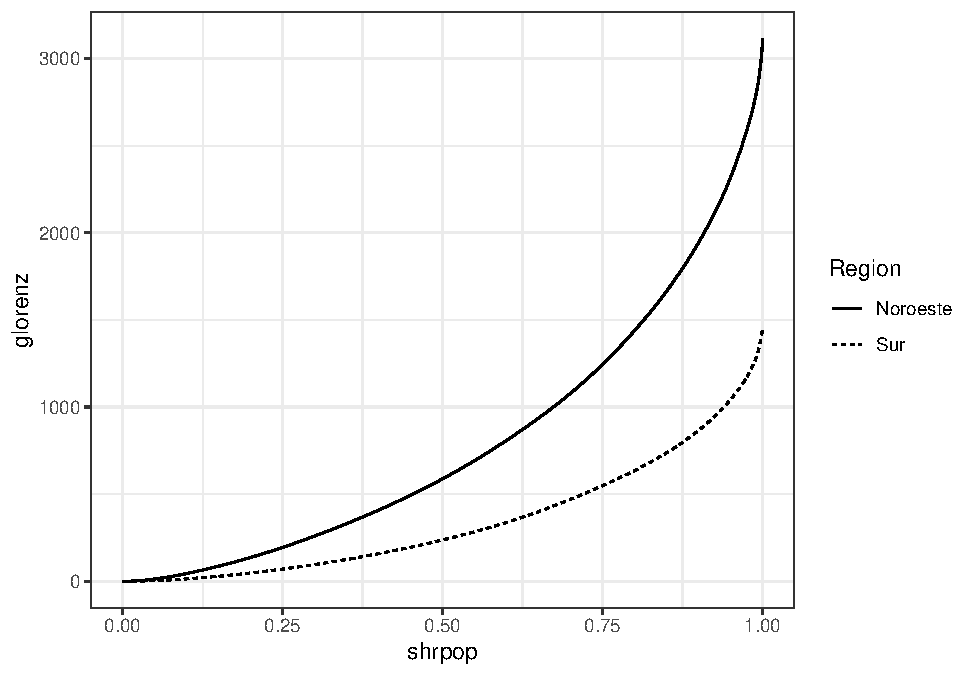
\includegraphics[width=0.8\linewidth]{_main_files/figure-latex/unnamed-chunk-29-1}

\hypertarget{cap-2.8}{%
\section{Curva de Incidencia}\label{cap-2.8}}

\#\#\#- (pág. 83)

En este apartado se muestra cómo pueden estimarse las curvas de incidencia del crecimiento que aparecen en la figura 2.21 del texto. A modo de ejemplo, se computa la curva de incidencia del crecimiento para Argentina entre 1992 y 2006, utilizando percentiles del ingreso per cápita familiar. Para ello el lector deberá descargar dichas bases en su directorio de trabajo.

La idea básica será generar un bucle que en cada repetición cargue una base, la ordene por ipcf, genere el porcentaje de población acumulado, en base a este identifique el percentil de ingreso que corresponde y finalmente estime la media del ingreso en percentil. Dado que tenemos dos bases distintas, el bucle iterará dos veces.

Para implementarlo se propone utilizar una lista (objeto tipo \emph{list}), en la que la EPH de cada año va a ser un elemento distinto. Así el primer elemento de esa lista corresponderá a toda la base de 1992 y el segundo, a toda la base del 2006. Para señalar el primer y segundo elemento nos valemos de un contador \emph{i} que en la primer iteración del bucle valdrá uno, y al que iremos sumando de uno en uno, por lo que en la segunda tomará valor dos. Por eso la expresión \texttt{bases\_mod{[}{[}i{]}{]}} será equivalente a decir ``elemento 1 de la lista \emph{bases\_mod}'' en la primera iteración y ``elemento 2 de la lista \emph{bases\_mod}'' en la segunda iteración. Con esto logramos que en vez de ordenar, generar y cambiar variables sobre un dataframe estático, lo hagamos sucesivamente sobre dataframes distintos contenidos en un lista ``madre'', que aquí llamamos \emph{bases\_mod}.

Nuestro bucle irá iterando sobre \emph{j}, que al igual que \emph{i} cambiará de valor en cada vuelta. En la primera será 92 y en la segunda 06 y nos servirá para indicar con qué base trabajar. Así \texttt{read.dta()} tiene como argumento la función \texttt{paste()} que une el prefijo \emph{``arg''} al año de la base correspondiente (\emph{j}), generando, junto con el prefijo \emph{``dta''}, un string igual al nombre de la base completa. De esta forma logramos cambiar el nombre en cada iteración para cargar bases de años diferentes.

Dado que estamos trabajando con años distintos debemos prever que necesitaremos ajustar los valores de ingresos por inflación. Por eso en caso de que la base sea la del 92, se multiplica el ipcf por el factor de ajuste (2.099). Esto se debe hacer solo en el caso de la base de 1992 y la manera de instrumentarlo es diciéndole a R que ese cambio debe realizarse solo cuando j sea igual a 92 -\texttt{if\ (j=="92")}-.

Una vez cargada la base, logrado el ajuste por inflación, aplicamos los mismos pasos que antes para ordenar por ipcf a la población y calcular el porcentaje acumulado. Con ese porcentaje acumulado generaremos los percentiles anidando un bucle a nuestro bucle inicial, que hará 100 repeticiones en cada EPH. En cada una de ellas asignará los percentiles en base a \emph{shrpop} ayudándose de la variable \emph{z} multiplicada por 0.01. La razón es sencilla: si queremos generar percentiles (n=100), necesitamos 100 cuantiles por lo que cada cuantil se asigna de a intervalos de población acumulada iguales a 0.01 (1/100). Así por ejemplo, cuando z sea igual a 20, \texttt{(z-1)*0.01} será igual a 0.19 y \texttt{z*0.01} a 0.20, por lo que caerán en este cuantil veinte, todos aquellos individuos que ordenados por ingreso, estén entre el 19 y el 20 por ciento de población acumulada. Dado que empleamos el comando \texttt{ifelse()}, para las obserservaciones restantes que caen fuera de este intervalo, se mantendrá el valor que ya traía la variable \emph{``percentil''}. Es por esto que antes del bucle, la generamos como vacía, para luego ir rellenándola sucesivamente. \emph{z} continuará incrementándose de a uno, hasta llegar a 100, donde asigne el último percentil a aquellas personas que quedaron ultimas en nuestra ordenación, ya que poseían los ingresos mas alto. Al considerar a este 1\% de la población faltante, se habrá acumulado al 100\%. Finalmente el último paso, consiste en reducir todo el dataframe a 100 observaciones correspondientes a los 100 percentiles recién creados y calcular la media del ingreso de las personas que pertenezcan a cada percentil.

\begin{Shaded}
\begin{Highlighting}[]
\NormalTok{bases\_mod }\OtherTok{\textless{}{-}} \FunctionTok{list}\NormalTok{() }\CommentTok{\#lista vacia en la que se guardaran los cambios}

\NormalTok{i }\OtherTok{\textless{}{-}} \DecValTok{1}              \CommentTok{\#contador para iterar sobre los elementos de la lista}

\CommentTok{\#j tomará valor 92 y 06}
\ControlFlowTok{for}\NormalTok{ (j }\ControlFlowTok{in} \FunctionTok{c}\NormalTok{(}\StringTok{"92"}\NormalTok{,}\StringTok{"06"}\NormalTok{))\{     }
  
  \CommentTok{\#cargo base}
\NormalTok{  bases\_mod[[i]] }\OtherTok{\textless{}{-}} \FunctionTok{read.dta}\NormalTok{(data\_dir }\SpecialCharTok{\%+\%} \FunctionTok{paste}\NormalTok{(}\StringTok{"Arg/bases/arg"}\NormalTok{,j,}\StringTok{"\_cedlas.dta"}\NormalTok{, }\AttributeTok{sep =}\StringTok{""}\NormalTok{)) }\SpecialCharTok{\%\textgreater{}\%} 
                    \FunctionTok{filter}\NormalTok{(cohh}\SpecialCharTok{==}\DecValTok{1} \SpecialCharTok{\&} \SpecialCharTok{!}\FunctionTok{is.na}\NormalTok{(ipcf) }\SpecialCharTok{\&}\NormalTok{ ipcf}\SpecialCharTok{!=}\DecValTok{0}\NormalTok{)}
  
  \CommentTok{\#ajuste por inflación para el año 92 solamente}
  \ControlFlowTok{if}\NormalTok{ (j}\SpecialCharTok{==}\StringTok{"92"}\NormalTok{)\{}
    
\NormalTok{      bases\_mod[[i]] }\OtherTok{\textless{}{-}}\NormalTok{ bases\_mod[[i]] }\SpecialCharTok{\%\textgreater{}\%} \FunctionTok{mutate}\NormalTok{(}\AttributeTok{ipcf=}\NormalTok{ipcf}\SpecialCharTok{*}\FloatTok{2.099}\NormalTok{)}
    
\NormalTok{  \}}
  
  \CommentTok{\#ordenar según ipcf}
\NormalTok{  bases\_mod[[i]] }\OtherTok{\textless{}{-}}\NormalTok{ bases\_mod[[i]] }\SpecialCharTok{\%\textgreater{}\%} \FunctionTok{arrange}\NormalTok{(ipcf)}
  
  \CommentTok{\#computar porcentaje de población}
\NormalTok{  bases\_mod[[i]] }\OtherTok{\textless{}{-}}\NormalTok{ bases\_mod[[i]] }\SpecialCharTok{\%\textgreater{}\%} \FunctionTok{mutate}\NormalTok{(}\AttributeTok{shrpop=}\FunctionTok{cumsum}\NormalTok{(pondera)}\SpecialCharTok{/}\FunctionTok{sum}\NormalTok{(pondera))}
  
  \CommentTok{\#identificar percentil de ipcf}
\NormalTok{  bases\_mod[[i]] }\OtherTok{\textless{}{-}}\NormalTok{ bases\_mod[[i]] }\SpecialCharTok{\%\textgreater{}\%} \FunctionTok{mutate}\NormalTok{(}\AttributeTok{percentile=}\DecValTok{0}\NormalTok{)  }\CommentTok{\#esto es equivalente a gen percentile=. en stata}
   
      \ControlFlowTok{for}\NormalTok{ (z }\ControlFlowTok{in} \DecValTok{1}\SpecialCharTok{:}\DecValTok{100}\NormalTok{)\{  }\CommentTok{\#bucle anidado: itera 100 veces para cada una de las bases }
    
\NormalTok{        bases\_mod[[i]] }\OtherTok{\textless{}{-}}\NormalTok{ bases\_mod[[i]] }\SpecialCharTok{\%\textgreater{}\%} \FunctionTok{mutate}\NormalTok{(}\AttributeTok{percentile=}\FunctionTok{ifelse}\NormalTok{((shrpop}\SpecialCharTok{\textgreater{}}\NormalTok{(z}\DecValTok{{-}1}\NormalTok{)}\SpecialCharTok{*}\FloatTok{0.01} \SpecialCharTok{\&}\NormalTok{ shrpop}\SpecialCharTok{\textless{}=}\NormalTok{z}\SpecialCharTok{*}\FloatTok{0.01}\NormalTok{), z, percentile)) }
        
\NormalTok{      \}  }
  
\NormalTok{  bases\_mod[[i]] }\OtherTok{\textless{}{-}}\NormalTok{ bases\_mod[[i]] }\SpecialCharTok{\%\textgreater{}\%} \FunctionTok{group\_by}\NormalTok{(percentile) }\SpecialCharTok{\%\textgreater{}\%} 
                                       \FunctionTok{summarise}\NormalTok{(}\AttributeTok{ipcf=}\FunctionTok{wtd.mean}\NormalTok{(ipcf, }\AttributeTok{w=}\NormalTok{pondera, }\AttributeTok{na.rm=}\ConstantTok{TRUE}\NormalTok{))}
  
\NormalTok{  i}\OtherTok{=}\NormalTok{i}\SpecialCharTok{+}\DecValTok{1}  
  
\NormalTok{\}}
\end{Highlighting}
\end{Shaded}

Cuando el bucle finaliza, podemos ``recuperar'' como dataframes los elementos almacenados en nuestra lista \emph{``bases\_mod''}. El primero corresponde a los ingresos promedios de cada percentil construidos con la base de 1992 y el segundo con la de 2006.

\begin{Shaded}
\begin{Highlighting}[]
\CommentTok{\#recupero las bases de cada año como respectivos elementos de la lista}
\NormalTok{arg92 }\OtherTok{\textless{}{-}} \FunctionTok{data.frame}\NormalTok{(bases\_mod[[}\DecValTok{1}\NormalTok{]])}
\NormalTok{arg06 }\OtherTok{\textless{}{-}} \FunctionTok{data.frame}\NormalTok{(bases\_mod[[}\DecValTok{2}\NormalTok{]])}

\FunctionTok{head}\NormalTok{(arg92)}
\end{Highlighting}
\end{Shaded}

\begin{verbatim}
##   percentile      ipcf
## 1          1  40.71898
## 2          2  69.34599
## 3          3  84.42000
## 4          4  99.58729
## 5          5 112.42315
## 6          6 122.64216
\end{verbatim}

Para finalizar la estimación, debemos calcular el cambio porcentual en el ingreso promedio de cada percentil entre estos años. Para ello necesitaremos juntar ambos dataframes en un solo, a partir de la variable percentil, que se encuentra en ambos. Con el comando \texttt{merge()} unificamos las bases y le asignamos un sufijo que nos permita identificar cada columna. Hecho esto ya podemos calcular el cambio porcentual en el ipcf promedio y graficarlo para cada percentil.

\begin{Shaded}
\begin{Highlighting}[]
\CommentTok{\#junto bases, asigno nombres y calculo el cambio porcentual}
\NormalTok{change }\OtherTok{\textless{}{-}} \FunctionTok{merge}\NormalTok{(arg92, arg06, }\AttributeTok{by=}\StringTok{"percentile"}\NormalTok{, }\AttributeTok{suffix=}\FunctionTok{c}\NormalTok{(}\StringTok{"\_92"}\NormalTok{, }\StringTok{"\_06"}\NormalTok{)) }\SpecialCharTok{\%\textgreater{}\%} 
          \FunctionTok{mutate}\NormalTok{(}\AttributeTok{change=}\NormalTok{( (ipcf\_06}\SpecialCharTok{/}\NormalTok{ipcf\_92) }\SpecialCharTok{{-}}\DecValTok{1}\NormalTok{)}\SpecialCharTok{*}\DecValTok{100}\NormalTok{) }


\DocumentationTok{\#\# Figura 2.21 {-} Curva de incidencia ipcf}
\FunctionTok{ggplot}\NormalTok{(change,}
       \FunctionTok{aes}\NormalTok{(}\AttributeTok{x=}\NormalTok{percentile, }\AttributeTok{y=}\NormalTok{change))}\SpecialCharTok{+}
  \FunctionTok{geom\_line}\NormalTok{(}\AttributeTok{size=}\FloatTok{1.2}\NormalTok{, }\AttributeTok{color=}\StringTok{"darkcyan"}\NormalTok{) }\SpecialCharTok{+}
  \FunctionTok{geom\_hline}\NormalTok{(}\AttributeTok{yintercept =} \DecValTok{0}\NormalTok{, }\AttributeTok{linetype=}\StringTok{"dashed"}\NormalTok{) }\SpecialCharTok{+}
  \FunctionTok{theme\_bw}\NormalTok{()}
\end{Highlighting}
\end{Shaded}

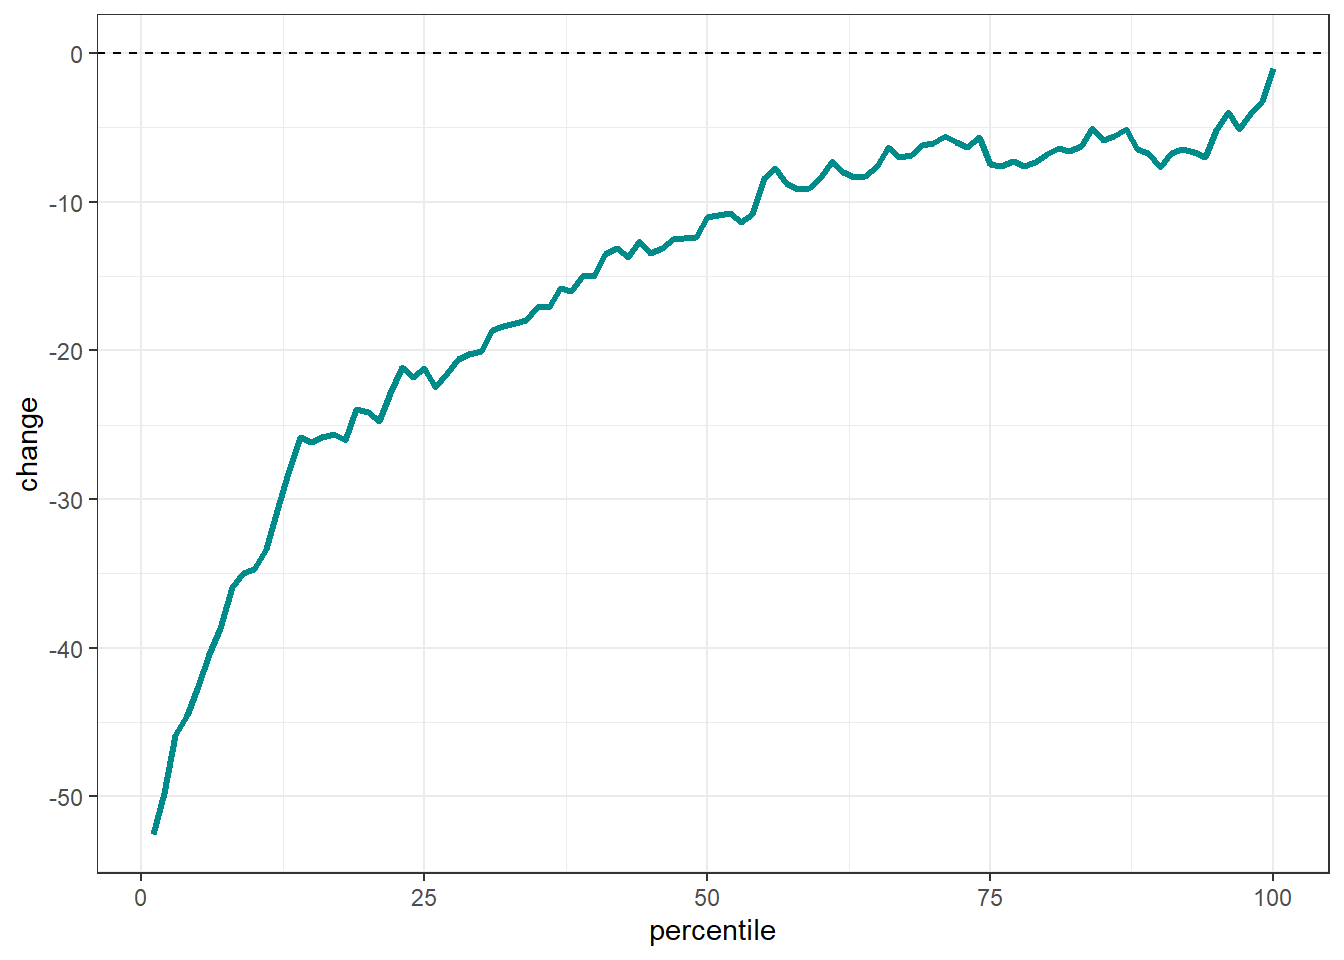
\includegraphics[width=0.8\linewidth]{_main_files/figure-latex/unnamed-chunk-32-1}

En el caso particuar de esta figura, las magnitudes son diferentes a los reportados orginalmente en el capitulo del libro, pero las interpretaciones se mantienen. La tasa de crecimiento del ingreso
real está completamente por debajo del eje horizontal, denotando una pérdida de ingresos reales, que dada la pendiente positiva de la curva implica caídas proporcionales del ingreso más grandes a medida que vamos descendiendo hacia estratos más pobres de la distribución. Es claro que la desigualdad de ingresos debe haber aumentado en Argentina en ese período.

\hypertarget{capuxedtulo-3}{%
\chapter{Capítulo 3}\label{capuxedtulo-3}}

\hypertarget{variables-y-fuentes-de-informaciuxf3n}{%
\section*{Variables y fuentes de información}\label{variables-y-fuentes-de-informaciuxf3n}}

\hypertarget{escrito-por-cristian-bonavida-1}{%
\subsubsection*{Escrito por: Cristian Bonavida}\label{escrito-por-cristian-bonavida-1}}
\addcontentsline{toc}{subsubsection}{Escrito por: Cristian Bonavida}

\hypertarget{last-update-0272021-1}{%
\subsubsection*{Last Update: 02/7/2021}\label{last-update-0272021-1}}
\addcontentsline{toc}{subsubsection}{Last Update: 02/7/2021}

~

\emph{Códigos escritos en base a los apéndices del libro ``Pobreza y Desigualdad en América Latina'' de Gasparini, Cicowiez y Sosa Escudero. El objeto de este material es reproducir la rutina de códigos para STATA presentada en el libro al lenguaje R. Este material es solo de caracter complementario a las explicaciones y detalles conceptuales que se presentan en el libro de texto y los apéndices}

~

\hypertarget{set-inicial-1}{%
\section*{Set Inicial}\label{set-inicial-1}}
\addcontentsline{toc}{section}{Set Inicial}

Cargo las librerias, limpio environment, defino el path y atajo para función paste

\begin{Shaded}
\begin{Highlighting}[]
\FunctionTok{library}\NormalTok{(dplyr)}
\FunctionTok{library}\NormalTok{(tidyverse) }\CommentTok{\# Data wrangling}
\FunctionTok{library}\NormalTok{(tidygraph)}
\FunctionTok{library}\NormalTok{(readxl)}
\FunctionTok{library}\NormalTok{(ggplot2)}
\FunctionTok{library}\NormalTok{(foreign)}
\FunctionTok{library}\NormalTok{(TAM)}

\FunctionTok{rm}\NormalTok{(}\AttributeTok{list=}\FunctionTok{ls}\NormalTok{())    }\CommentTok{\#empiezo limpiando todo }

\StringTok{"\%+\%"} \OtherTok{\textless{}{-}} \ControlFlowTok{function}\NormalTok{(x,y) }\FunctionTok{paste}\NormalTok{(x,y,}\AttributeTok{sep =} \StringTok{""}\NormalTok{)      }\CommentTok{\# defino un shorcut parar concat de texto}
\NormalTok{data\_dir }\OtherTok{\textless{}{-}} \StringTok{"C:/Users/HP/Desktop/CEDLAS {-} UNLP/Apendices en R/Material libro/encuestas{-}cedlas/Encuestas/"}  \CommentTok{\#seteo directorio }
\end{Highlighting}
\end{Shaded}

~

\hypertarget{cociente-de-cuantiles}{%
\section{Cociente de cuantiles}\label{cociente-de-cuantiles}}

\#\#\#- (pág. 151-152)

El siguiente bloque de código puede utilizarse para computar el cociente de quintiles extremos presentado en el cuadro 3.2 del texto del libro, el cual es un indicador de desigualdad extendido en la literatura, que denota la magnitud de las brechas entre los más ricos y más pobres. Para iniciar se importa la base desde el formato STATA utilizando de la librería \texttt{foreing}, el comando \texttt{read.dta()}. Luego hago una limpieza de la base, ordeno las observaciones según la variable ``ipcf'', filtro ingresos nulos y por último computo el porcentaje acumulado por población, como se vio en el capítulo anterior.

\begin{Shaded}
\begin{Highlighting}[]
\CommentTok{\#cargo base}
\NormalTok{mex06 }\OtherTok{\textless{}{-}} \FunctionTok{read.dta}\NormalTok{(data\_dir }\SpecialCharTok{\%+\%} \StringTok{"Mex/2006/bases/mex06\_cedlas.dta"}\NormalTok{)  }

\CommentTok{\#elimino observaciones incoherentes o con ingreso missing}
\NormalTok{mex06 }\OtherTok{\textless{}{-}}\NormalTok{ mex06 }\SpecialCharTok{\%\textgreater{}\%} \FunctionTok{filter}\NormalTok{(cohh}\SpecialCharTok{==}\DecValTok{1}\NormalTok{, }\SpecialCharTok{!}\FunctionTok{is.na}\NormalTok{(ipcf)) }

\CommentTok{\#ordenar por ipcf, filtrar ingresos nulos y computar \% de población}
\NormalTok{df }\OtherTok{\textless{}{-}}\NormalTok{  mex06  }\SpecialCharTok{\%\textgreater{}\%} \FunctionTok{arrange}\NormalTok{(ipcf) }\SpecialCharTok{\%\textgreater{}\%} \FunctionTok{filter}\NormalTok{(ipcf}\SpecialCharTok{\textgreater{}}\DecValTok{0}\NormalTok{) }\SpecialCharTok{\%\textgreater{}\%} 
       \FunctionTok{mutate}\NormalTok{(}\AttributeTok{shrpop=}\FunctionTok{cumsum}\NormalTok{(pondera)}\SpecialCharTok{/}\FunctionTok{sum}\NormalTok{(pondera))}
\end{Highlighting}
\end{Shaded}

A partir de allí genero la variable quintil en el dataframe, que vale 1 para el 20\% más pobre de la población, 2 para el 20\% siguiente, y así sucesivamente. El comando \texttt{ifelse} permite evaluar el porcentaje acumulado de población en cada observación y le otorga el valor del quintil correspondiente en caso afirmativo, o deja la variable inalterada en caso negativo. La lógica detrás es idéntica a la vista para generar percentiles dentro del bucle en la estimación de las curvas de incidencia (\protect\hyperlink{cap-2.8}{sección 2.8}).

\begin{Shaded}
\begin{Highlighting}[]
\NormalTok{df}\SpecialCharTok{$}\NormalTok{quintil }\OtherTok{=} \DecValTok{0}
\NormalTok{df}\SpecialCharTok{$}\NormalTok{quintil }\OtherTok{=} \FunctionTok{ifelse}\NormalTok{(df}\SpecialCharTok{$}\NormalTok{shrpop}\SpecialCharTok{\textless{}=}\FloatTok{0.2}\NormalTok{, }\DecValTok{1}\NormalTok{, df}\SpecialCharTok{$}\NormalTok{quintil)}
\NormalTok{df}\SpecialCharTok{$}\NormalTok{quintil }\OtherTok{=} \FunctionTok{ifelse}\NormalTok{(df}\SpecialCharTok{$}\NormalTok{shrpop}\SpecialCharTok{\textgreater{}} \FloatTok{0.2} \SpecialCharTok{\&}\NormalTok{ df}\SpecialCharTok{$}\NormalTok{shrpop}\SpecialCharTok{\textless{}=} \FloatTok{0.4}\NormalTok{, }\DecValTok{2}\NormalTok{, df}\SpecialCharTok{$}\NormalTok{quintil)}
\NormalTok{df}\SpecialCharTok{$}\NormalTok{quintil }\OtherTok{=} \FunctionTok{ifelse}\NormalTok{(df}\SpecialCharTok{$}\NormalTok{shrpop}\SpecialCharTok{\textgreater{}} \FloatTok{0.4} \SpecialCharTok{\&}\NormalTok{ df}\SpecialCharTok{$}\NormalTok{shrpop}\SpecialCharTok{\textless{}=} \FloatTok{0.6}\NormalTok{, }\DecValTok{3}\NormalTok{, df}\SpecialCharTok{$}\NormalTok{quintil)}
\NormalTok{df}\SpecialCharTok{$}\NormalTok{quintil }\OtherTok{=} \FunctionTok{ifelse}\NormalTok{(df}\SpecialCharTok{$}\NormalTok{shrpop}\SpecialCharTok{\textgreater{}} \FloatTok{0.6} \SpecialCharTok{\&}\NormalTok{ df}\SpecialCharTok{$}\NormalTok{shrpop}\SpecialCharTok{\textless{}=} \FloatTok{0.8}\NormalTok{, }\DecValTok{4}\NormalTok{, df}\SpecialCharTok{$}\NormalTok{quintil)}
\NormalTok{df}\SpecialCharTok{$}\NormalTok{quintil }\OtherTok{=} \FunctionTok{ifelse}\NormalTok{(df}\SpecialCharTok{$}\NormalTok{shrpop}\SpecialCharTok{\textgreater{}} \FloatTok{0.8} \SpecialCharTok{\&}\NormalTok{ df}\SpecialCharTok{$}\NormalTok{shrpop}\SpecialCharTok{\textless{}=} \DecValTok{1}\NormalTok{,   }\DecValTok{5}\NormalTok{, df}\SpecialCharTok{$}\NormalTok{quintil)}
\end{Highlighting}
\end{Shaded}

Para terminar computamos el ingreso promedio ponderado para las observaciones del quintil 1 y 5. Aquí la expresión \emph{\texttt{{[}df\$quintil==1{]}}} actúa como filtro. De esta manera el comando le pide a R considerar los valores de la variable \emph{ipcf} y \emph{pondera} que corresponden a observaciones que cumplen la condición, en este caso de pertenecer al quintil 1. Por último calculamos el ratio de estos dos valores e imprimimos el resultado. Para mayor claridad siempre se recomienda redondear los valores a imprimir, utilizando el comando \texttt{round()}.

\begin{Shaded}
\begin{Highlighting}[]
\NormalTok{ipcf\_q1 }\OtherTok{=} \FunctionTok{weighted.mean}\NormalTok{(df}\SpecialCharTok{$}\NormalTok{ipcf[df}\SpecialCharTok{$}\NormalTok{quintil}\SpecialCharTok{==}\DecValTok{1}\NormalTok{], df}\SpecialCharTok{$}\NormalTok{pondera[df}\SpecialCharTok{$}\NormalTok{quintil}\SpecialCharTok{==}\DecValTok{1}\NormalTok{], }\AttributeTok{na.rm =} \ConstantTok{TRUE}\NormalTok{)}
\NormalTok{ipcf\_q5 }\OtherTok{=} \FunctionTok{weighted.mean}\NormalTok{(df}\SpecialCharTok{$}\NormalTok{ipcf[df}\SpecialCharTok{$}\NormalTok{quintil}\SpecialCharTok{==}\DecValTok{5}\NormalTok{], df}\SpecialCharTok{$}\NormalTok{pondera[df}\SpecialCharTok{$}\NormalTok{quintil}\SpecialCharTok{==}\DecValTok{5}\NormalTok{], }\AttributeTok{na.rm =} \ConstantTok{TRUE}\NormalTok{)}
\NormalTok{ratq51 }\OtherTok{=}\NormalTok{ ipcf\_q5}\SpecialCharTok{/}\NormalTok{ipcf\_q1}

\FunctionTok{paste}\NormalTok{(}\StringTok{"ratq51 = "}\NormalTok{, ratq51)}
\end{Highlighting}
\end{Shaded}

\begin{verbatim}
## [1] "ratq51 =  13.4341399453849"
\end{verbatim}

\begin{Shaded}
\begin{Highlighting}[]
\FunctionTok{paste}\NormalTok{(}\StringTok{"ratq51 = "}\NormalTok{, }\FunctionTok{round}\NormalTok{(ratq51, }\AttributeTok{digits =} \DecValTok{2}\NormalTok{))}
\end{Highlighting}
\end{Shaded}

\begin{verbatim}
## [1] "ratq51 =  13.43"
\end{verbatim}

El valor obtenido indica que el ingreso en el quintil 5 es 13.4 veces más alto que el del quintil 1, para el año 2006 en México considerando el total país.

~

\hypertarget{cap-3.2}{%
\section{Replicar programa ratq51}\label{cap-3.2}}

\#\#\#- (pág. 153-154)

En la siguientes líneas de código proponemos escribir una función que permite computar el cociente de quintiles extremos muy fácilmente; simplemente se lo invoca indicando la base de datos, la variable de la que se quieren computar quintiles, y opcionalmente la variable de ponderación y la condición \texttt{if}. Una función en R es similar a lo que en STATA llamaríamos un programa, es decir un conjunto de instrucciones que se guardan en la memoria y que pueden ser fácilmente replicables en distintas bases de datos y para distintas variables.

La función puede resultar un poco extensa por lo que aquí enumeraremos las líneas de código para mayor claridad. Para iniciar la función, en la primer línea debemos especificar sus argumentos, que en este caso son: un dataframe (objeto \emph{``df''}), una variable (objeto \emph{``varname''}) y opcionalmente una variable de ponderación y una condición (objetos \emph{``var\_pondera''} y \emph{``condicion''}). Para llamar a esta función entonces siempre tendremos que, como mínimo, especificar los dos objetos iniciales.

La siguiente línea se asegura que la base de datos \emph{``df''} que hemos especificado siempre sea almacenado como un objeto del tipo \emph{data frame} en un objeto llamado \emph{``aux''} que creamos en el entorno de la función. La noción de entorno es importante para comprender el resto del código. A los fines de nuestro código diremos que un entorno es un espacio determinando en el que se almacenan distintas clases de objetos que R acepta y, en el cual estos tienen un significado, un valor o simplemente existen como objetos. En R pueden ``coexistir'' environmets distintos, a los cuales se le asigna un nivel o prioridad\footnote{Para los usuarios que no esten tan familiarizados con las nociones de \emph{Environment} y \emph{Non-Standard Evaluation} se recomienda revisar las siguientes referencias para un tratamiento mas detallado.

  *\url{http://adv-r.had.co.nz/Environments.html\#environments}

  *\url{http://adv-r.had.co.nz/Computing-on-the-language.html}

  *\url{https://advanced-r-solutions-ed1.netlify.app/non-standard-evaluation.html\#non-standard-evaluation-in-subse}}. Volviendo a nuestro código, cuando a R le especificamos, por ejemplo, el objeto \emph{``varname''}, R buscará si este está definido en el \emph{entorno o environment} general del programa como prioridad, y no en el entorno o espacio de la función, que es más acotado que el anterior. Por lo tanto aquí necesitamos evitar este comportamiento y lograr que R no busque evaluar al objeto por fuera del ambito de la función. El comando \texttt{substitute()} le indica a R que considere al objeto con su nombre literal. Así cuando \emph{``varname''} sea definida, por ejemplo, como la variable ``ipcf'', R no buscará a qué es equivalente el objeto ``ipcf'' en su memoria sino que tomará el nombre dado como literal. Luego la función \texttt{eval()} le indica a R que ese nombre debe evaluarlo, es decir buscarlo o identificarlo, dentro del dataframe \emph{``aux''} que hemos definido en nuestra función. De esta forma nos aseguramos de que R considera correctamente las variables dentro de la base de datos que estamos especificando, y por lo tanto que nuestros argumentos sean válidos dentro del ámbito de la función. Es decir que no entren en conflicto con otros objetos similares o definidos previamente en el environment más amplio del programa.

Utilizando estas dos funciones, en la línea 7 almacenamos todos los valores de ipcf a partir de los cuales luego ordenamos la base en la siguiente línea. Como la condición es un argumento opcional debemos evaluar si esta fue indicada, en términos de R si no es un objeto nulo (línea 12). Si no lo es, luego en la línea 14 verificamos que esté correctamente especificada, escribiendo una sentencia que será VERDADERA cuando al evaluar de forma silenciosa la condición, dé como resultado un error \emph{(``try-error'')}. En ese caso entonces se imprime un mensaje que ayuda al usuario a identificar donde se encuentra el problema. En caso de que el resultado no sea del tipo error, la condición será aceptada por lo que filtramos el objeto \emph{``aux''} de acuerdo a la especificación dada. Para ello nos valemos de la función \texttt{parse} que convierte la condición que era del tipo \emph{``string''} al tipo \emph{``expression''}, lo que la vuelve compatible de ser evaluada como sentencia, nuevamente con la función \texttt{eval()} dentro de \texttt{filter()}.

De forma similar procedemos con el ponderador en la línea 24. Si no fue especificado (objeto nulo), entonces vale 1 para todas las observaciones, a partir de crear una variable que llamamos ``w'' que pasará a ser nuestra variable ponderador, pero que será inocua a los fines del cálculo. En el objeto \emph{``var\_pondera\_store''} almacenamos esta secuencia de valores 1. En cambio, si el ponderador fue especificado entonces ese objeto almacena los valores correspondientes a la variable señalada, sin entrar en conflicto con un posible objeto del mismo nombre definido fuero del espacio de la función.

En la línea 38 actualizamos el objeto que almacena los valores de ipcf (en caso de que se hayan filtrado valores de acuerdo a la condición), y en la siguiente ordenamos el dataframe \emph{``aux''}, para calcular como antes el porcentaje acumulado de población. Por último definimos inicialmente a la variable ``quintil'' como valores 0. En la línea 45 replicamos la asignación del quintil que se realizó antes con el comando \texttt{ifelse} pero ahora de forma iterativa, cambiando en cada iteración los valores del quintil y de población acumulada.

Por último al igual que antes calculamos el ratio entre quintiles extremos filtrando las observaciones del primer y quinto quintil. La única diferencia es que aquí nuevamente debemos asegurarnos de que los valores promedios y los ponderadores se evalúen para estas observaciones y sólo en el contexto o espacio de la función. Para finalizar imprimimos los resultados.

\begin{Shaded}
\begin{Highlighting}[numbers=left,,]
\NormalTok{ratq51 }\OtherTok{\textless{}{-}} \ControlFlowTok{function}\NormalTok{(df, varname, }\AttributeTok{var\_pondera=}\ConstantTok{NULL}\NormalTok{, }\AttributeTok{condicion=}\ConstantTok{NULL}\NormalTok{) \{}
    
\NormalTok{    aux }\OtherTok{\textless{}{-}} \FunctionTok{as.data.frame}\NormalTok{(df) }
    
    \CommentTok{\#substitute() toma literal el nombre sin asignarle ningun valor posible y }
    \CommentTok{\#eval() evalua ese nombre en el contexto del data frame que es el primer arguento definido}
\NormalTok{    varname\_store }\OtherTok{\textless{}{-}} \FunctionTok{eval}\NormalTok{(}\FunctionTok{substitute}\NormalTok{(varname), aux) }
\NormalTok{    aux }\OtherTok{\textless{}{-}}\NormalTok{ aux }\SpecialCharTok{\%\textgreater{}\%} \FunctionTok{arrange}\NormalTok{(varname\_store)}
    
    
    \CommentTok{\#la condición es un argumento opcional}
    \ControlFlowTok{if}\NormalTok{(}\SpecialCharTok{!}\FunctionTok{is.null}\NormalTok{(}\FunctionTok{substitute}\NormalTok{(condicion))) \{}
      
       \ControlFlowTok{if}\NormalTok{(}\FunctionTok{is}\NormalTok{(}\FunctionTok{try}\NormalTok{(}\FunctionTok{eval}\NormalTok{(}\FunctionTok{substitute}\NormalTok{(condicion)), }\AttributeTok{silent =} \ConstantTok{TRUE}\NormalTok{ ), }\StringTok{"try{-}error"}\NormalTok{))}
        
          \FunctionTok{stop}\NormalTok{(}\StringTok{"ERROR: la condicion debe especificarse como character (entre comillas)"}\NormalTok{)}
      
\NormalTok{          aux }\OtherTok{\textless{}{-}}\NormalTok{ aux }\SpecialCharTok{\%\textgreater{}\%} \FunctionTok{filter}\NormalTok{(}\FunctionTok{eval}\NormalTok{(}\FunctionTok{parse}\NormalTok{(}\AttributeTok{text=}\NormalTok{condicion)))  }\CommentTok{\#convierte la condicion de tipo string al tipo }
                                                            \CommentTok{\#expression y luego la evalua dentro del filter}
\NormalTok{    \}}
    
    
    \CommentTok{\#set pondera= 1 si no está especificado}
    \ControlFlowTok{if}\NormalTok{(}\FunctionTok{is.null}\NormalTok{(}\FunctionTok{substitute}\NormalTok{(var\_pondera))) \{                           }
      
\NormalTok{      aux }\OtherTok{\textless{}{-}}\NormalTok{ aux }\SpecialCharTok{\%\textgreater{}\%} \FunctionTok{mutate}\NormalTok{(}\AttributeTok{w=}\DecValTok{1}\NormalTok{)}
\NormalTok{      var\_pondera}\OtherTok{=}\FunctionTok{substitute}\NormalTok{(w)}
\NormalTok{      var\_pondera\_store }\OtherTok{\textless{}{-}} \FunctionTok{eval}\NormalTok{(}\FunctionTok{substitute}\NormalTok{(var\_pondera), aux)}
      
\NormalTok{      \} }\ControlFlowTok{else}\NormalTok{ \{}
      
\NormalTok{      var\_pondera\_store }\OtherTok{\textless{}{-}} \FunctionTok{eval}\NormalTok{(}\FunctionTok{substitute}\NormalTok{(var\_pondera), aux)}
      
\NormalTok{    \}}
    
    
    \CommentTok{\#ordeno y genero quintiles}
\NormalTok{    varname\_store }\OtherTok{\textless{}{-}} \FunctionTok{eval}\NormalTok{(}\FunctionTok{substitute}\NormalTok{(varname), aux)}
\NormalTok{    aux }\OtherTok{\textless{}{-}}\NormalTok{ aux }\SpecialCharTok{\%\textgreater{}\%} \FunctionTok{arrange}\NormalTok{(varname\_store) }\SpecialCharTok{\%\textgreater{}\%}
                   \FunctionTok{mutate}\NormalTok{(}\AttributeTok{shrpop=}\FunctionTok{cumsum}\NormalTok{(var\_pondera\_store)}\SpecialCharTok{/}\FunctionTok{sum}\NormalTok{(var\_pondera\_store)) }\SpecialCharTok{\%\textgreater{}\%} 
                   \FunctionTok{mutate}\NormalTok{(}\AttributeTok{quintil=}\DecValTok{0}\NormalTok{)}
    
    \ControlFlowTok{for}\NormalTok{ (i }\ControlFlowTok{in} \DecValTok{1}\SpecialCharTok{:}\DecValTok{5}\NormalTok{) \{}
      
\NormalTok{     aux }\OtherTok{\textless{}{-}}\NormalTok{ aux }\SpecialCharTok{\%\textgreater{}\%} \FunctionTok{mutate}\NormalTok{(}\AttributeTok{quintil=}\FunctionTok{ifelse}\NormalTok{((shrpop}\SpecialCharTok{\textgreater{}}\NormalTok{(i}\DecValTok{{-}1}\NormalTok{)}\SpecialCharTok{*}\FloatTok{0.2} \SpecialCharTok{\&}\NormalTok{ shrpop}\SpecialCharTok{\textless{}=}\NormalTok{i}\SpecialCharTok{*}\FloatTok{0.2}\NormalTok{), i, quintil)) }
      
\NormalTok{    \}  }
    
    
    \CommentTok{\#ingreso promedio quintil 1 }
\NormalTok{    aux\_1 }\OtherTok{\textless{}{-}}\NormalTok{ aux }\SpecialCharTok{\%\textgreater{}\%} \FunctionTok{filter}\NormalTok{(quintil}\SpecialCharTok{==}\DecValTok{1}\NormalTok{) }
\NormalTok{    media\_q1 }\OtherTok{=} \FunctionTok{weighted.mean}\NormalTok{(}\FunctionTok{eval}\NormalTok{(}\FunctionTok{substitute}\NormalTok{(varname),aux\_1), }\FunctionTok{eval}\NormalTok{(}\FunctionTok{substitute}\NormalTok{(var\_pondera), aux\_1), }\AttributeTok{na.rm =} \ConstantTok{TRUE}\NormalTok{)}
\NormalTok{    media\_q1 }\OtherTok{=} \FunctionTok{round}\NormalTok{(media\_q1, }\AttributeTok{digits =} \DecValTok{2}\NormalTok{)}
    \CommentTok{\#ingreso promedio quintil 5 }
\NormalTok{    aux\_5 }\OtherTok{\textless{}{-}}\NormalTok{ aux }\SpecialCharTok{\%\textgreater{}\%} \FunctionTok{filter}\NormalTok{(quintil}\SpecialCharTok{==}\DecValTok{5}\NormalTok{) }
\NormalTok{    media\_q5 }\OtherTok{=} \FunctionTok{weighted.mean}\NormalTok{(}\FunctionTok{eval}\NormalTok{(}\FunctionTok{substitute}\NormalTok{(varname),aux\_5), }\FunctionTok{eval}\NormalTok{(}\FunctionTok{substitute}\NormalTok{(var\_pondera), aux\_5), }\AttributeTok{na.rm =} \ConstantTok{TRUE}\NormalTok{)}
\NormalTok{    media\_q5 }\OtherTok{=} \FunctionTok{round}\NormalTok{(media\_q5, }\AttributeTok{digits =} \DecValTok{2}\NormalTok{)}
    \CommentTok{\#ratio}
\NormalTok{    ratq\_51 }\OtherTok{=}\NormalTok{ media\_q5}\SpecialCharTok{/}\NormalTok{media\_q1}
    
    
    \FunctionTok{print}\NormalTok{(}\FunctionTok{paste}\NormalTok{(}\StringTok{"media quintil 5"}\NormalTok{, }\FunctionTok{substitute}\NormalTok{(varname), }\StringTok{"= "}\NormalTok{, media\_q5))}
    \FunctionTok{print}\NormalTok{(}\FunctionTok{paste}\NormalTok{(}\StringTok{"media quintil 1"}\NormalTok{, }\FunctionTok{substitute}\NormalTok{(varname), }\StringTok{"= "}\NormalTok{, media\_q1))}
    \FunctionTok{print}\NormalTok{(}\FunctionTok{paste}\NormalTok{(}\StringTok{"ratio = "}\NormalTok{, }\FunctionTok{round}\NormalTok{(ratq\_51, }\AttributeTok{digits =} \DecValTok{2}\NormalTok{)))}
    
  
\NormalTok{\}}
\end{Highlighting}
\end{Shaded}

Al correr el código, R almacenará en la memoria esta función, a la cual podremos llamar simplemente indicando los argumentos relevantes. En las líneas siguientes se detallan algunos ejemplos de cómo replicar la función bajo distintas especificaciones.

\begin{Shaded}
\begin{Highlighting}[]
\CommentTok{\#No especifica condicion}
\FunctionTok{ratq51}\NormalTok{(mex06, ipcf, pondera)  }
\end{Highlighting}
\end{Shaded}

\begin{verbatim}
## [1] "media quintil 5 ipcf =  6655.49"
## [1] "media quintil 1 ipcf =  448.38"
## [1] "ratio =  14.84"
\end{verbatim}

\begin{Shaded}
\begin{Highlighting}[]
\CommentTok{\#Especifica condicion}
\FunctionTok{ratq51}\NormalTok{(mex06, ipcf, pondera, }\StringTok{"ipcf\textgreater{}0"}\NormalTok{) }
\end{Highlighting}
\end{Shaded}

\begin{verbatim}
## [1] "media quintil 5 ipcf =  6707.64"
## [1] "media quintil 1 ipcf =  499.3"
## [1] "ratio =  13.43"
\end{verbatim}

\begin{Shaded}
\begin{Highlighting}[]
\CommentTok{\#Especifica condición doble}
\FunctionTok{ratq51}\NormalTok{(mex06, ipcf, pondera, }\StringTok{"region==4 | region==2"}\NormalTok{)  }
\end{Highlighting}
\end{Shaded}

\begin{verbatim}
## [1] "media quintil 5 ipcf =  6420.24"
## [1] "media quintil 1 ipcf =  499.01"
## [1] "ratio =  12.87"
\end{verbatim}

\begin{Shaded}
\begin{Highlighting}[]
\CommentTok{\#Especifica incorrectamente la condición}
\FunctionTok{ratq51}\NormalTok{(}\AttributeTok{df=}\NormalTok{mex06, ipcf, pondera, region}\SpecialCharTok{==}\DecValTok{4} \SpecialCharTok{\&}\NormalTok{ urbano}\SpecialCharTok{==}\DecValTok{1}\NormalTok{) }
\end{Highlighting}
\end{Shaded}

\begin{verbatim}
## Error in ratq51(df = mex06, ipcf, pondera, region == 4 & urbano == 1): ERROR: la condicion debe especificarse como character (entre comillas)
\end{verbatim}

\begin{Shaded}
\begin{Highlighting}[]
\CommentTok{\#No especifica pondera}
\FunctionTok{ratq51}\NormalTok{(}\AttributeTok{df=}\NormalTok{mex06, }\AttributeTok{varname=}\NormalTok{ipcf, }\AttributeTok{condicion=}\StringTok{"region==4 \& urbano==1"}\NormalTok{)  }
\end{Highlighting}
\end{Shaded}

\begin{verbatim}
## [1] "media quintil 5 ipcf =  6384.76"
## [1] "media quintil 1 ipcf =  594.14"
## [1] "ratio =  10.75"
\end{verbatim}

\begin{Shaded}
\begin{Highlighting}[]
\CommentTok{\#Identifica los argumentos explicitamente por nombre }
\FunctionTok{ratq51}\NormalTok{(}\AttributeTok{df=}\NormalTok{mex06, }\AttributeTok{varname=}\NormalTok{ipcf, }\AttributeTok{var\_pondera=}\NormalTok{pondera, }\AttributeTok{condicion=}\StringTok{"region==4 \& urbano==1"}\NormalTok{) }
\end{Highlighting}
\end{Shaded}

\begin{verbatim}
## [1] "media quintil 5 ipcf =  6640.93"
## [1] "media quintil 1 ipcf =  586.57"
## [1] "ratio =  11.32"
\end{verbatim}

~

\hypertarget{replicar-programa-gcuan}{%
\section{Replicar programa gcuan}\label{replicar-programa-gcuan}}

\#\#\#- (pág. 154-155)

El bloque de código a continuación permite identificar cuantiles de cualquier variable. En términos del programa ``ratq51'', nos permite generar variables similares a quintil pero que pueden identificar quintiles, deciles, ventiles, percentiles, etc.

Por esta razón, esta función tendrá más argumentos, aquí además de los anteriores debemos detallar la cantidad de cuantiles a generar (objeto \emph{``num''}) y la variable que los almacena (\emph{``newvar''}). Luego el código y la secuencia son idénticos a la de la función anterior, salvo porque aquí definimos de una manera alternativa y más directa a los valores del poderador, pero en esencia replica lo visto antes hasta la línea 40. A partir de aquí el objeto \emph{``num''} indica cuantos cuantiles deben generarse, hace iterar al bucle \emph{``num''} cantidad de veces, y define los intervalos de población acumulada de forma equivalente. Por ejemplo, si queremos generar deciles (num=10), necesitamos 10 cuantiles y cada cuantil se asigna de a intervalos de población acumulada iguales a 0.10 (1/10).

Posteriormente en la línea 50 generamos el reporte (objeto \emph{``show''}) que imprimiremos como resultado. Este calcula la media ponderada, el desvió standard ponderado y la cantidad de observaciones en base la variable especificada en \emph{``varname''} y \emph{``var\_pondera''}. Los objetos \emph{``my\_var''} y \emph{``my\_var2''} son variables auxiliares que generamos en el data frame solo con el objeto de facilitarnos el cálculo directo. Para terminar cambiamos el nombre de la variable que hasta ahora generamos como ``quintil'' por el nombre indicado en el argumento. El comando \texttt{names(aux)} trae todos los nombres de este dataframe y con la expresión \emph{\texttt{{[}names(aux)\ ==\ "quintil"{]}}} elegimos de esos nombres, solo el que coincide con la palabra ``quintil''. A esta columna específica le asignamos el nombre dado como argumento, tomando la expresión literal con \texttt{substitute()} pasada al formato string mediante la función \texttt{paste()}. En resumen la línea 59 sería el equivalente de escribir en la consola \emph{\texttt{aux\$quintil\ \textless{}-\ "nombre\_asignado"}}, con la dificultad de que debemos hacerlo dentro del espacio de la función, respetando los argumentos dados. La línea 60 por su parte elimina del output final la variable shrpop.

Para finalizar especificamos que esta función no solo debe imprimirnos los resultados guardados en \emph{``show''}, sino que además debe devolver una base de datos nueva. El comando \texttt{return(aux)} le dice a R que el resultado será el objeto \emph{``aux''} en sí mismo, es decir obtendremos la base original con una nueva columna llamada \emph{``newvar''} que es la que esta función genera.

\begin{Shaded}
\begin{Highlighting}[numbers=left,,]
\NormalTok{gcuan }\OtherTok{\textless{}{-}} \ControlFlowTok{function}\NormalTok{(df, varname, }\AttributeTok{var\_pondera=}\ConstantTok{NULL}\NormalTok{, }\AttributeTok{condicion=}\ConstantTok{NULL}\NormalTok{, num, newvar) \{}
  
\NormalTok{  aux }\OtherTok{\textless{}{-}} \FunctionTok{as.data.frame}\NormalTok{(df) }
  
\NormalTok{  varname\_store }\OtherTok{\textless{}{-}} \FunctionTok{eval}\NormalTok{(}\FunctionTok{substitute}\NormalTok{(varname), aux) }
\NormalTok{  aux }\OtherTok{\textless{}{-}}\NormalTok{ aux }\SpecialCharTok{\%\textgreater{}\%} \FunctionTok{arrange}\NormalTok{(varname\_store)}
  
  
  \CommentTok{\#la condición es un argumento opcional}
  \ControlFlowTok{if}\NormalTok{(}\SpecialCharTok{!}\FunctionTok{is.null}\NormalTok{(}\FunctionTok{substitute}\NormalTok{(condicion))) \{}
      
     \ControlFlowTok{if}\NormalTok{(}\FunctionTok{is}\NormalTok{(}\FunctionTok{try}\NormalTok{(}\FunctionTok{eval}\NormalTok{(}\FunctionTok{substitute}\NormalTok{(condicion)), }\AttributeTok{silent =} \ConstantTok{TRUE}\NormalTok{ ), }\StringTok{"try{-}error"}\NormalTok{))}
        
        \FunctionTok{stop}\NormalTok{(}\StringTok{"ERROR: la condicion debe especificarse como character (entre comillas)"}\NormalTok{)}
      
\NormalTok{        aux }\OtherTok{\textless{}{-}}\NormalTok{ aux }\SpecialCharTok{\%\textgreater{}\%} \FunctionTok{filter}\NormalTok{(}\FunctionTok{eval}\NormalTok{(}\FunctionTok{parse}\NormalTok{(}\AttributeTok{text=}\NormalTok{condicion)))     }
                                                              
\NormalTok{   \}}
  
  
  \CommentTok{\#set pondera= 1 si no está especificado}
  \ControlFlowTok{if}\NormalTok{(}\FunctionTok{is.null}\NormalTok{(}\FunctionTok{substitute}\NormalTok{(var\_pondera))) \{                           }
    
\NormalTok{    var\_pondera\_store }\OtherTok{\textless{}{-}} \FunctionTok{c}\NormalTok{(}\FunctionTok{rep}\NormalTok{(}\DecValTok{1}\NormalTok{, }\FunctionTok{nrow}\NormalTok{(aux)))}
    
\NormalTok{    \} }\ControlFlowTok{else}\NormalTok{ \{}
    
\NormalTok{    var\_pondera\_store }\OtherTok{\textless{}{-}} \FunctionTok{eval}\NormalTok{(}\FunctionTok{substitute}\NormalTok{(var\_pondera), aux)}
    
\NormalTok{  \}}
  
  
  \CommentTok{\#ordeno y genero shrpop}
\NormalTok{  varname\_store }\OtherTok{\textless{}{-}} \FunctionTok{eval}\NormalTok{(}\FunctionTok{substitute}\NormalTok{(varname), aux)}
\NormalTok{  aux }\OtherTok{\textless{}{-}}\NormalTok{ aux }\SpecialCharTok{\%\textgreater{}\%} \FunctionTok{arrange}\NormalTok{(varname\_store) }\SpecialCharTok{\%\textgreater{}\%} 
    \FunctionTok{mutate}\NormalTok{(}\AttributeTok{shrpop=}\FunctionTok{cumsum}\NormalTok{(var\_pondera\_store)}\SpecialCharTok{/}\FunctionTok{sum}\NormalTok{(var\_pondera\_store)) }\SpecialCharTok{\%\textgreater{}\%}
    \FunctionTok{mutate}\NormalTok{(}\AttributeTok{quintil=}\DecValTok{0}\NormalTok{)}
  
  \CommentTok{\#genero cuantiles en base a lo indicado}
\NormalTok{  shareq }\OtherTok{=} \DecValTok{1}\SpecialCharTok{/}\NormalTok{num}
  
  \ControlFlowTok{for}\NormalTok{ (i }\ControlFlowTok{in} \DecValTok{1}\SpecialCharTok{:}\NormalTok{num) \{}
    
\NormalTok{    aux }\OtherTok{\textless{}{-}}\NormalTok{ aux }\SpecialCharTok{\%\textgreater{}\%} \FunctionTok{mutate}\NormalTok{(}\AttributeTok{quintil=}\FunctionTok{ifelse}\NormalTok{((shrpop}\SpecialCharTok{\textgreater{}}\NormalTok{(i}\DecValTok{{-}1}\NormalTok{)}\SpecialCharTok{*}\NormalTok{shareq }\SpecialCharTok{\&}\NormalTok{ shrpop}\SpecialCharTok{\textless{}=}\NormalTok{i}\SpecialCharTok{*}\NormalTok{shareq), i, quintil))}
    
\NormalTok{  \}}
  
  
  \CommentTok{\#armo la información que se imprime en la consola}
\NormalTok{  show }\OtherTok{\textless{}{-}}\NormalTok{ aux }\SpecialCharTok{\%\textgreater{}\%} \FunctionTok{mutate}\NormalTok{(}\AttributeTok{my\_var=}\NormalTok{varname\_store,}
                         \AttributeTok{my\_var2=}\NormalTok{var\_pondera\_store) }\SpecialCharTok{\%\textgreater{}\%} \FunctionTok{group\_by}\NormalTok{(quintil) }\SpecialCharTok{\%\textgreater{}\%}
                  \FunctionTok{summarise}\NormalTok{(}\AttributeTok{mean =} \FunctionTok{weighted\_mean}\NormalTok{(my\_var, my\_var2),}
                             \AttributeTok{std =} \FunctionTok{weighted\_sd}\NormalTok{(my\_var, my\_var2),}
                             \AttributeTok{obs =} \FunctionTok{sum}\NormalTok{(my\_var2))}
  
  
  \CommentTok{\#renombro variable al nombre indicado como argumento y descarto shrpop}
  \FunctionTok{names}\NormalTok{(show)[}\FunctionTok{names}\NormalTok{(show) }\SpecialCharTok{==} \StringTok{"quintil"}\NormalTok{] }\OtherTok{\textless{}{-}} \FunctionTok{paste}\NormalTok{(}\FunctionTok{substitute}\NormalTok{(newvar))}
  \FunctionTok{names}\NormalTok{(aux)[}\FunctionTok{names}\NormalTok{(aux) }\SpecialCharTok{==} \StringTok{"quintil"}\NormalTok{] }\OtherTok{\textless{}{-}} \FunctionTok{paste}\NormalTok{(}\FunctionTok{substitute}\NormalTok{(newvar))}
\NormalTok{  aux}\SpecialCharTok{$}\NormalTok{shrpop }\OtherTok{\textless{}{-}} \ConstantTok{NULL}
  
  \CommentTok{\#outputs}
  \FunctionTok{print.data.frame}\NormalTok{(show)}
  \FunctionTok{return}\NormalTok{(aux)}
  
  
\NormalTok{\}}
\end{Highlighting}
\end{Shaded}

A diferencia entonces de la anterior, esta función devuelve no sólo un resultado impreso sino un objeto, por lo que ahora debemos especificar cómo lo nombramos. Si lo llamamos de la misma manera que el argumento que le pasamos a la función simplemente estamos pisando este objeto y añadiéndole una nueva variable. Otra alternativa es crear un nuevo dataframe con otro nombre.

\begin{Shaded}
\begin{Highlighting}[]
\CommentTok{\#Especifica todo correctamente y crea nuevo dataframe}
\NormalTok{mex06\_bis }\OtherTok{\textless{}{-}} \FunctionTok{gcuan}\NormalTok{(}\AttributeTok{df=}\NormalTok{mex06, }\AttributeTok{varname=}\NormalTok{ipcf, }\AttributeTok{var\_pondera=}\NormalTok{pondera, }\AttributeTok{condicion=}\StringTok{"ipcf\textgreater{}0"}\NormalTok{, }\AttributeTok{num=}\DecValTok{5}\NormalTok{, }\AttributeTok{newvar=}\NormalTok{quintil)}
\end{Highlighting}
\end{Shaded}

\begin{verbatim}
##   quintil      mean       std      obs
## 1       1  499.2978  197.3755 20372798
## 2       2 1011.4695  136.6778 20383133
## 3       3 1539.5536  172.7480 20385227
## 4       4 2382.6530  345.4059 20380795
## 5       5 6707.6362 6532.2051 20381791
\end{verbatim}

\begin{Shaded}
\begin{Highlighting}[]
\CommentTok{\#No especifica correctamente la condición}
\NormalTok{mex06\_bis }\OtherTok{\textless{}{-}} \FunctionTok{gcuan}\NormalTok{(}\AttributeTok{df=}\NormalTok{mex06, }\AttributeTok{varname=}\NormalTok{ipcf, }\AttributeTok{var\_pondera=}\NormalTok{pondera, }\AttributeTok{condicion=}\NormalTok{region}\SpecialCharTok{==}\DecValTok{4}\NormalTok{, }\AttributeTok{num=}\DecValTok{5}\NormalTok{, }\AttributeTok{newvar=}\NormalTok{quintil)}
\end{Highlighting}
\end{Shaded}

\begin{verbatim}
## Error in gcuan(df = mex06, varname = ipcf, var_pondera = pondera, condicion = region == : ERROR: la condicion debe especificarse como character (entre comillas)
\end{verbatim}

\begin{Shaded}
\begin{Highlighting}[]
\CommentTok{\#No especifica condición}
\NormalTok{mex06\_bis }\OtherTok{\textless{}{-}} \FunctionTok{gcuan}\NormalTok{(}\AttributeTok{df=}\NormalTok{mex06, }\AttributeTok{varname=}\NormalTok{ipcf, }\AttributeTok{var\_pondera=}\NormalTok{pondera, }\AttributeTok{num=}\DecValTok{5}\NormalTok{, }\AttributeTok{newvar=}\NormalTok{quintil)}
\end{Highlighting}
\end{Shaded}

\begin{verbatim}
##   quintil      mean       std      obs
## 1       1  448.3757  222.9768 20677642
## 2       2  986.9415  137.2255 20677386
## 3       3 1518.1792  172.0445 20676646
## 4       4 2357.4796  343.4104 20678111
## 5       5 6655.4937 6499.4356 20679061
\end{verbatim}

\begin{Shaded}
\begin{Highlighting}[]
\CommentTok{\#No especifica pondera}
\NormalTok{mex06\_bis }\OtherTok{\textless{}{-}} \FunctionTok{gcuan}\NormalTok{(}\AttributeTok{df=}\NormalTok{mex06, }\AttributeTok{varname=}\NormalTok{ipcf, }\AttributeTok{num=}\DecValTok{5}\NormalTok{, }\AttributeTok{newvar=}\NormalTok{quintil)}
\end{Highlighting}
\end{Shaded}

\begin{verbatim}
##   quintil      mean       std   obs
## 1       1  363.0791  202.9644 16400
## 2       2  900.1146  135.1091 16401
## 3       3 1424.6686  177.6839 16401
## 4       4 2273.6985  346.6132 16401
## 5       5 6401.7186 6319.9421 16401
\end{verbatim}

\begin{Shaded}
\begin{Highlighting}[]
\CommentTok{\#Especifica todo correctamente y reemplaza el dataframe dado}
\NormalTok{mex06 }\OtherTok{\textless{}{-}} \FunctionTok{gcuan}\NormalTok{(}\AttributeTok{df=}\NormalTok{mex06, }\AttributeTok{varname=}\NormalTok{ipcf, }\AttributeTok{var\_pondera=}\NormalTok{pondera, }\AttributeTok{condicion=}\StringTok{"ipcf\textgreater{}0"}\NormalTok{, }\AttributeTok{num=}\DecValTok{5}\NormalTok{, }\AttributeTok{newvar=}\NormalTok{quintil)}
\end{Highlighting}
\end{Shaded}

\begin{verbatim}
##   quintil      mean       std      obs
## 1       1  499.2978  197.3755 20372798
## 2       2 1011.4695  136.6778 20383133
## 3       3 1539.5536  172.7480 20385227
## 4       4 2382.6530  345.4059 20380795
## 5       5 6707.6362 6532.2051 20381791
\end{verbatim}

~

\hypertarget{tamauxf1o-de-los-hogares}{%
\section{Tamaño de los hogares}\label{tamauxf1o-de-los-hogares}}

\#\#\#- (pág. 156)

El código siguiente puede utilizarse para computar las estadísticas sobre proporción de hogares unipersonales y multipersonales presentadas en el cuadro 3.4 del texto. Con este código podremos calcular qué proporción del total de hogares se compone de 1, 2, 3, 4,\ldots n miembros y combinado con los códigos anteriores, analizar cómo esta configuración cambia al agrupar por regiones, percentil de ingreso, condición de pobreza, etc. Como ya es habitual, en la primera línea indicamos con qué base iremos a trabajar. Luego ordenamos los hogares de forma creciente en base a su identificador \emph{``id''} y en forma decreciente respecto la variable \emph{``jefe''}. Dado que esta vale 1 solo para el jefe de hogar y 0 para todo el resto, la primera observación por \emph{``id''} corresponderá siempre a la cabeza del hogar. La función \texttt{duplicated()} genera una variable que será \emph{FALSE} para la primera observación dentro de cada id, indicando que esta no está duplicada por ser la primera, pero será \emph{TRUE} para todas las que siguen, ya que se identificó antes una observación con el mismo id. De esta manera hacemos un ``tag'' del jefe de hogar y mantenemos todos los demás miembros. En el caso de que no nos interesa mantener en nuestra base el resto de las observaciones, estos pasos se simplifican a un simple filtrado por jefe de hogar.

Luego generamos la variable tamaño solo para el jefe de hogar en base la cantidad de miembros que viven con él, utilizando la función \texttt{case\_when()}. Así, por ejemplo, cuando la observación corresponda al jefe y la cantidad de miembros sea igual a 3, en ese caso la variable \emph{``tamaño''} valdrá 3. Por último armamos nuestra tabla resultado filtrando a los jefes de hogar, agrupando por tamaño y sumando la cantidad de hogares (porque tenemos una sola observación por hogar) y la frecuencia relativa en cada caso.

\begin{Shaded}
\begin{Highlighting}[]
\CommentTok{\#indico con qué base de hogares voy a trabajar}
\NormalTok{df }\OtherTok{\textless{}{-}}\NormalTok{ mex06 }

\CommentTok{\#ordeno por id y jefe (decreciente) e identifico al jefe de hogar}
\NormalTok{df }\OtherTok{\textless{}{-}}\NormalTok{ df }\SpecialCharTok{\%\textgreater{}\%} \FunctionTok{arrange}\NormalTok{(id, }\FunctionTok{desc}\NormalTok{(jefe)) }\SpecialCharTok{\%\textgreater{}\%}
          \FunctionTok{mutate}\NormalTok{(}\AttributeTok{hh=}\FunctionTok{duplicated}\NormalTok{(id))      }\CommentTok{\#idéntico a: egen hh=tag() en stata}

\CommentTok{\#genero tamaño sólo para los jefes de hogar}
\NormalTok{df }\OtherTok{\textless{}{-}}\NormalTok{ df }\SpecialCharTok{\%\textgreater{}\%} \FunctionTok{mutate}\NormalTok{(tamaño}\OtherTok{=}\FunctionTok{case\_when}\NormalTok{(miembros}\SpecialCharTok{==}\DecValTok{1} \SpecialCharTok{\&}\NormalTok{ hh}\SpecialCharTok{==}\ConstantTok{FALSE} \SpecialCharTok{\textasciitilde{}} \DecValTok{1}\NormalTok{,}
\NormalTok{                                     miembros}\SpecialCharTok{==}\DecValTok{2} \SpecialCharTok{\&}\NormalTok{ hh}\SpecialCharTok{==}\ConstantTok{FALSE} \SpecialCharTok{\textasciitilde{}} \DecValTok{2}\NormalTok{,}
\NormalTok{                                     miembros}\SpecialCharTok{==}\DecValTok{3} \SpecialCharTok{\&}\NormalTok{ hh}\SpecialCharTok{==}\ConstantTok{FALSE} \SpecialCharTok{\textasciitilde{}} \DecValTok{3}\NormalTok{,}
\NormalTok{                                     miembros}\SpecialCharTok{==}\DecValTok{4} \SpecialCharTok{\&}\NormalTok{ hh}\SpecialCharTok{==}\ConstantTok{FALSE} \SpecialCharTok{\textasciitilde{}} \DecValTok{4}\NormalTok{,}
\NormalTok{                                     miembros}\SpecialCharTok{==}\DecValTok{5} \SpecialCharTok{\&}\NormalTok{ hh}\SpecialCharTok{==}\ConstantTok{FALSE} \SpecialCharTok{\textasciitilde{}} \DecValTok{5}\NormalTok{,}
\NormalTok{                                     miembros}\SpecialCharTok{\textgreater{}=}\DecValTok{6} \SpecialCharTok{\&}\NormalTok{ hh}\SpecialCharTok{==}\ConstantTok{FALSE} \SpecialCharTok{\textasciitilde{}} \DecValTok{6}\NormalTok{))}

\CommentTok{\#tabla con resultados}
\NormalTok{table }\OtherTok{\textless{}{-}}\NormalTok{ df }\SpecialCharTok{\%\textgreater{}\%} \FunctionTok{filter}\NormalTok{(hh}\SpecialCharTok{==}\ConstantTok{FALSE}\NormalTok{) }\SpecialCharTok{\%\textgreater{}\%} \FunctionTok{group\_by}\NormalTok{(tamaño) }\SpecialCharTok{\%\textgreater{}\%} \FunctionTok{summarise}\NormalTok{(}\AttributeTok{N =} \FunctionTok{sum}\NormalTok{(pondera)) }\SpecialCharTok{\%\textgreater{}\%} 
                                                           \FunctionTok{mutate}\NormalTok{(}\AttributeTok{freq =}\NormalTok{ N}\SpecialCharTok{*}\DecValTok{100}\SpecialCharTok{/}\FunctionTok{sum}\NormalTok{(N))}
\NormalTok{table}
\end{Highlighting}
\end{Shaded}

\begin{verbatim}
## # A tibble: 6 x 3
##   tamaño       N  freq
##    <dbl>   <int> <dbl>
## 1      1 2070859  8.15
## 2      2 3717891 14.6 
## 3      3 4815417 18.9 
## 4      4 5875572 23.1 
## 5      5 4422391 17.4 
## 6      6 4516967 17.8
\end{verbatim}

El objeto table almacena los resultados que se visualizan en la consola. A veces al imprimir los resultados estos no se visualizan con un formato muy amigable. A modo de extensión presentamos dos alternativas para refinar este aspecto. El paquete \texttt{formattable} nos permite, entre otras cosas, especificar el tipo de datos y el formato para distintas variables al generar el dataframe. Por su parte \texttt{print.data.frame} nos da una visualización más limpia. Incorporando este aspecto el código para nuestra tabla sería:

\begin{Shaded}
\begin{Highlighting}[]
\CommentTok{\#install.packages("formattable")}
\FunctionTok{library}\NormalTok{(formattable)}

\NormalTok{table }\OtherTok{\textless{}{-}}\NormalTok{ df }\SpecialCharTok{\%\textgreater{}\%} \FunctionTok{filter}\NormalTok{(hh}\SpecialCharTok{==}\ConstantTok{FALSE}\NormalTok{) }\SpecialCharTok{\%\textgreater{}\%} \FunctionTok{group\_by}\NormalTok{(tamaño) }\SpecialCharTok{\%\textgreater{}\%} \FunctionTok{summarise}\NormalTok{(}\AttributeTok{N =} \FunctionTok{accounting}\NormalTok{(}\FunctionTok{sum}\NormalTok{(pondera), }\AttributeTok{digits =} \DecValTok{0}\NormalTok{)) }\SpecialCharTok{\%\textgreater{}\%} 
                                                              \FunctionTok{mutate}\NormalTok{(}\AttributeTok{freq =} \FunctionTok{percent}\NormalTok{(N}\SpecialCharTok{/}\FunctionTok{sum}\NormalTok{(N)))}
\FunctionTok{print.data.frame}\NormalTok{(table)}
\end{Highlighting}
\end{Shaded}

\begin{verbatim}
##   tamaño         N   freq
## 1      1 2,070,859  8.15%
## 2      2 3,717,891 14.63%
## 3      3 4,815,417 18.94%
## 4      4 5,875,572 23.11%
## 5      5 4,422,391 17.40%
## 6      6 4,516,967 17.77%
\end{verbatim}

Además de agregarle esta customización, para los usuarios que utilizan ``Rmarkdown'' habitualmente, es posible mostrar los resultados con una visualización amigable de forma sencilla.

\begin{Shaded}
\begin{Highlighting}[]
\NormalTok{rmarkdown}\SpecialCharTok{::}\FunctionTok{paged\_table}\NormalTok{(table)}
\end{Highlighting}
\end{Shaded}

~

\hypertarget{la-distribuciuxf3n-intrahogar}{%
\section{La distribución intrahogar}\label{la-distribuciuxf3n-intrahogar}}

\#\#\#- (pág. 157)

El fragmento de código siguiente puede utilizarse para generar resultados similares a los presentados en el cuadro 3.7 del texto, que muestra cómo se modifica la desigualdad calculada a través del cociente de deciles extremos cuando cambia la distribución del ingreso hacia el interior del hogar. Cabe recordar que la distribución del ingreso intrahogar se modifica mediante un impuesto proporcional al ingreso per cápita familiar combinado, con un subsidio que solo recibe el jefe de hogar. En la implementación, utilizamos quintiles en lugar de deciles ingreso.

En la primera línea cargamos la base, en este caso de Venezuela año 2006, limpiamos y ordenamos los hogares. Más abajo creamos el objeto \emph{``ty''} que toma el valor de la tasa del impuesto aplicada sobre el ipcf, el cual calculamos en la línea siguiente generando en el dataframe una nueva columna \emph{``impuesto''}. Posteriormente calculamos el valor del subsidio a otorgar, que surge de sumar el valor de los impuestos para los integrantes de un mismo hogar. En la línea siguiente modificamos la variable subsidio, haciendo que valga 0 para todo miembro distinto al jefe de hogar, de esta forma redistribuyendo el ingreso al interior del hogar. A todos se le hemos quitado una porción \emph{``ty''} que ahora la recibe solamente el jefe.

En la anteúltima línea creamos una variable para el nuevo valor de ingreso per cápita familiar, restando el impuesto y sumando el subsidio. Por último hacemos uso de nuestra función del ratio de quintiles para computar el cociente del ingreso promedio de los quintiles 5 y 1 como indicador de desigualdad, a partir del ingreso modificado.

\begin{Shaded}
\begin{Highlighting}[]
\NormalTok{ven06 }\OtherTok{\textless{}{-}} \FunctionTok{read.dta}\NormalTok{(data\_dir }\SpecialCharTok{\%+\%} \StringTok{"Ven/2006/bases/ven06\_cedlas.dta"}\NormalTok{)  }

\CommentTok{\#elimino observaciones incoherentes o con ingreso missing y ordeno}
\NormalTok{df }\OtherTok{\textless{}{-}}\NormalTok{ ven06 }\SpecialCharTok{\%\textgreater{}\%} \FunctionTok{filter}\NormalTok{(cohh}\SpecialCharTok{==}\DecValTok{1}\NormalTok{, }\SpecialCharTok{!}\FunctionTok{is.na}\NormalTok{(ipcf)) }\SpecialCharTok{\%\textgreater{}\%} \FunctionTok{arrange}\NormalTok{(id)}

\CommentTok{\#tasa del impuesto}
\NormalTok{ty}\OtherTok{=}\FloatTok{0.1}

\CommentTok{\#impuesto al ipcf}
\NormalTok{df}\SpecialCharTok{$}\NormalTok{impuesto }\OtherTok{=}\NormalTok{ df}\SpecialCharTok{$}\NormalTok{ipcf}\SpecialCharTok{*}\NormalTok{ty    }\CommentTok{\#alternativa a escribir: df \textless{}{-} df \%\textgreater{}\% mutate(impuesto = ipcf*ty)}

\CommentTok{\#recaudación impuesto total por hogar}
\NormalTok{df }\OtherTok{\textless{}{-}}\NormalTok{ df }\SpecialCharTok{\%\textgreater{}\%} \FunctionTok{group\_by}\NormalTok{(id) }\SpecialCharTok{\%\textgreater{}\%} \FunctionTok{mutate}\NormalTok{(}\AttributeTok{subsidio =} \FunctionTok{sum}\NormalTok{(impuesto))}

\CommentTok{\#subsidio solo lo recibe el jefe de hogar }
\NormalTok{df}\SpecialCharTok{$}\NormalTok{subsidio }\OtherTok{\textless{}{-}} \FunctionTok{ifelse}\NormalTok{(df}\SpecialCharTok{$}\NormalTok{jefe}\SpecialCharTok{!=}\DecValTok{1}\NormalTok{, }\DecValTok{0}\NormalTok{, df}\SpecialCharTok{$}\NormalTok{subsidio)  }

\CommentTok{\#nuevo ipcf}
\NormalTok{df}\SpecialCharTok{$}\NormalTok{ipcf\_star }\OtherTok{=}\NormalTok{ df}\SpecialCharTok{$}\NormalTok{ipcf }\SpecialCharTok{{-}}\NormalTok{ df}\SpecialCharTok{$}\NormalTok{impuesto }\SpecialCharTok{+}\NormalTok{ df}\SpecialCharTok{$}\NormalTok{subsidio }

\FunctionTok{ratq51}\NormalTok{(df, ipcf\_star, pondera, }\StringTok{"ipcf\textgreater{}0"}\NormalTok{)  }
\end{Highlighting}
\end{Shaded}

\begin{verbatim}
## [1] "media quintil 5 ipcf_star =  842520.38"
## [1] "media quintil 1 ipcf_star =  79335.26"
## [1] "ratio =  10.62"
\end{verbatim}

A modo de comentario, un usuario mas familiarizado con el lenguaje podrá notar que las lineas que computan y asignan el subsidio puden resumirse en una sola, escribiendo.

\begin{Shaded}
\begin{Highlighting}[]
\NormalTok{df }\OtherTok{\textless{}{-}}\NormalTok{ df }\SpecialCharTok{\%\textgreater{}\%} \FunctionTok{group\_by}\NormalTok{(id) }\SpecialCharTok{\%\textgreater{}\%} \FunctionTok{mutate}\NormalTok{(}\AttributeTok{subsidio=}\FunctionTok{ifelse}\NormalTok{(jefe}\SpecialCharTok{!=}\DecValTok{1}\NormalTok{, }\DecValTok{0}\NormalTok{, }\FunctionTok{sum}\NormalTok{(impuesto)))}
\end{Highlighting}
\end{Shaded}

~

\hypertarget{cap-3.6}{%
\section{Empleo de ponderadores}\label{cap-3.6}}

\#\#\#- (pág. 157)

El bloque de código que sigue puede utilizarse para construir un cuadro como el 3.9 del texto, que muestra la relación entre el ingreso per cápita familiar y el valor de la variable de ponderación.

Dado que ya habíamos trabajado con la base de México, aquí no la volvemos a cargar. En la segunda línea genera la variable \emph{``shrobs''}, que contiene el porcentaje acumulado de observaciones, y que es distinta de \emph{``shrpop''} que contiene el acumulado de población usando el ponderador. Aquí la expresión \emph{\texttt{1:n()}} enumera secuencialmente las observaciones en orden de aparición mientras que \emph{\texttt{n()}} computa el total. El resto es habitual, generamos quintiles en base a los cuales luego agrupamos las observaciones para calcular la media de ingreso y el total de población en cada uno.

\begin{Shaded}
\begin{Highlighting}[]
\CommentTok{\#indico con que base de hogares voy a trabajar}
\NormalTok{df }\OtherTok{\textless{}{-}}\NormalTok{ mex06}

\CommentTok{\#ordenar por ipcf y computo porcentaje acumulado de observaciones}
\NormalTok{df }\OtherTok{\textless{}{-}}\NormalTok{ df }\SpecialCharTok{\%\textgreater{}\%} \FunctionTok{arrange}\NormalTok{(ipcf) }\SpecialCharTok{\%\textgreater{}\%}  \FunctionTok{mutate}\NormalTok{(}\AttributeTok{shrobs =} \DecValTok{1}\SpecialCharTok{:}\FunctionTok{n}\NormalTok{()}\SpecialCharTok{/}\FunctionTok{n}\NormalTok{()) }

\CommentTok{\#identificar quintiles de ipcf}
\NormalTok{df}\SpecialCharTok{$}\NormalTok{quintil }\OtherTok{=} \DecValTok{0}
\NormalTok{df}\SpecialCharTok{$}\NormalTok{quintil }\OtherTok{=} \FunctionTok{ifelse}\NormalTok{(df}\SpecialCharTok{$}\NormalTok{shrobs}\SpecialCharTok{\textless{}=} \FloatTok{0.2}\NormalTok{, }\DecValTok{1}\NormalTok{, df}\SpecialCharTok{$}\NormalTok{quintil)}
\NormalTok{df}\SpecialCharTok{$}\NormalTok{quintil }\OtherTok{=} \FunctionTok{ifelse}\NormalTok{(df}\SpecialCharTok{$}\NormalTok{shrobs}\SpecialCharTok{\textgreater{}}\FloatTok{0.2} \SpecialCharTok{\&}\NormalTok{ df}\SpecialCharTok{$}\NormalTok{shrobs}\SpecialCharTok{\textless{}=} \FloatTok{0.4}\NormalTok{, }\DecValTok{2}\NormalTok{, df}\SpecialCharTok{$}\NormalTok{quintil)}
\NormalTok{df}\SpecialCharTok{$}\NormalTok{quintil }\OtherTok{=} \FunctionTok{ifelse}\NormalTok{(df}\SpecialCharTok{$}\NormalTok{shrobs}\SpecialCharTok{\textgreater{}}\FloatTok{0.4} \SpecialCharTok{\&}\NormalTok{ df}\SpecialCharTok{$}\NormalTok{shrobs}\SpecialCharTok{\textless{}=} \FloatTok{0.6}\NormalTok{, }\DecValTok{3}\NormalTok{, df}\SpecialCharTok{$}\NormalTok{quintil)}
\NormalTok{df}\SpecialCharTok{$}\NormalTok{quintil }\OtherTok{=} \FunctionTok{ifelse}\NormalTok{(df}\SpecialCharTok{$}\NormalTok{shrobs}\SpecialCharTok{\textgreater{}}\FloatTok{0.6} \SpecialCharTok{\&}\NormalTok{ df}\SpecialCharTok{$}\NormalTok{shrobs}\SpecialCharTok{\textless{}=} \FloatTok{0.8}\NormalTok{, }\DecValTok{4}\NormalTok{, df}\SpecialCharTok{$}\NormalTok{quintil)}
\NormalTok{df}\SpecialCharTok{$}\NormalTok{quintil }\OtherTok{=} \FunctionTok{ifelse}\NormalTok{(df}\SpecialCharTok{$}\NormalTok{shrobs}\SpecialCharTok{\textgreater{}}\FloatTok{0.8} \SpecialCharTok{\&}\NormalTok{ df}\SpecialCharTok{$}\NormalTok{shrobs}\SpecialCharTok{\textless{}=} \DecValTok{1}\NormalTok{,   }\DecValTok{5}\NormalTok{, df}\SpecialCharTok{$}\NormalTok{quintil)}

\NormalTok{show }\OtherTok{\textless{}{-}}\NormalTok{ df }\SpecialCharTok{\%\textgreater{}\%} \FunctionTok{group\_by}\NormalTok{(quintil) }\SpecialCharTok{\%\textgreater{}\%} \FunctionTok{summarise}\NormalTok{(}\AttributeTok{mean =} \FunctionTok{accounting}\NormalTok{(}\FunctionTok{mean}\NormalTok{(ipcf), }\AttributeTok{digits =} \DecValTok{0}\NormalTok{),}
                                               \AttributeTok{means\_w =} \FunctionTok{accounting}\NormalTok{(}\FunctionTok{mean}\NormalTok{(pondera), }\AttributeTok{digits =} \DecValTok{0}\NormalTok{))}
\FunctionTok{print.data.frame}\NormalTok{(show)}
\end{Highlighting}
\end{Shaded}

\begin{verbatim}
##   quintil  mean means_w
## 1       1   413   1,038
## 2       2   926   1,269
## 3       3 1,449   1,345
## 4       4 2,302   1,344
## 5       5 6,457   1,319
\end{verbatim}

Seguidamente se calculan las tasas de pobreza con y sin ponderadores para el total del país y para cada una de las regiones de México en 2006, correspondientes al cuadro 3.10 del texto. En la primer línea el objeto \emph{``lp''} almacena el valor de la línea de pobreza, en base a la cual se genera la variable binaria \emph{``pobre''}, que vale 1 para los individuos debajo de este umbral (es decir, si \emph{ipcf \textless{} lp}) y 0 para el resto. La suma de esta variable arroja el número total de personas pobres en la muestra. Al multiplicarla por el ponderador obtenemos el número de personas pobres en la población y dividiendo por la población total del país nos devuelve la tasa de incidencia de la pobreza. En este caso el valor es de 13.57\%.

\begin{Shaded}
\begin{Highlighting}[]
\DocumentationTok{\#\#\#linea de pobreza us$2.5 Mexico 2006}
\NormalTok{lp}\OtherTok{=} \FloatTok{633.90918}

\CommentTok{\#identificar individuos pobres}
\NormalTok{df}\SpecialCharTok{$}\NormalTok{pobre }\OtherTok{=} \FunctionTok{ifelse}\NormalTok{(df}\SpecialCharTok{$}\NormalTok{ipcf}\SpecialCharTok{\textless{}}\NormalTok{lp, }\DecValTok{1}\NormalTok{, }\DecValTok{0}\NormalTok{)}

\CommentTok{\#total pais}
\FunctionTok{sum}\NormalTok{(df}\SpecialCharTok{$}\NormalTok{pobre}\SpecialCharTok{*}\NormalTok{df}\SpecialCharTok{$}\NormalTok{pondera)}\SpecialCharTok{*}\DecValTok{100}\SpecialCharTok{/}\FunctionTok{sum}\NormalTok{(df}\SpecialCharTok{$}\NormalTok{pondera)}
\end{Highlighting}
\end{Shaded}

\begin{verbatim}
## [1] 13.57454
\end{verbatim}

Las siguientes líneas calculan el mismo valor pero de una manera alternativa, almacenándolo en un dataframe, a partir de contabilizar la frecuencia absoluta y relativa de personas pobres y no pobres.

\begin{Shaded}
\begin{Highlighting}[]
\NormalTok{pobreza }\OtherTok{\textless{}{-}}\NormalTok{ df }\SpecialCharTok{\%\textgreater{}\%} \FunctionTok{group\_by}\NormalTok{(pobre) }\SpecialCharTok{\%\textgreater{}\%} \FunctionTok{summarise}\NormalTok{(}\AttributeTok{n =} \FunctionTok{accounting}\NormalTok{(}\FunctionTok{sum}\NormalTok{(pondera), }\AttributeTok{digits =} \DecValTok{0}\NormalTok{)) }\SpecialCharTok{\%\textgreater{}\%} 
                                      \FunctionTok{mutate}\NormalTok{(}\AttributeTok{tasa\_pobreza =} \FunctionTok{percent}\NormalTok{(n}\SpecialCharTok{/}\FunctionTok{sum}\NormalTok{(n))) }
\FunctionTok{print.data.frame}\NormalTok{(pobreza)}
\end{Highlighting}
\end{Shaded}

\begin{verbatim}
##   pobre          n tasa_pobreza
## 1     0 88,070,783       86.43%
## 2     1 13,832,961       13.57%
\end{verbatim}

Para replicar el mismo cálculo pero para las regiones del país, generamos un bucle que itera 8 veces, una vez por cada región. En cada vuelta del bucle se estima, de la misma forma que arriba, el valor de pobreza tanto ponderado como no ponderado. Para este segundo caso, el único paso adicional consiste en fijar la variable \emph{pondera} como igual a 1. Como vimos en la salida anterior de la tabla, en la 2da fila de la 3er columna se encuentra la tasa de incidencia de pobreza. Con la expresión \emph{\texttt{pobreza\_pondera{[}2,3{]}}} llamamos a este valor para guardarlo en el objeto \emph{``share\_p''}, luego de redondearlo a dos dígitos con el comando \texttt{round()}. Lo mismo hacemos para las estimaciones sin ponderar. Por último, imprimimos los resultados acompañados por una leyenda indicativa.

\begin{Shaded}
\begin{Highlighting}[]
\CommentTok{\#por region}
\ControlFlowTok{for}\NormalTok{ (i }\ControlFlowTok{in} \DecValTok{1}\SpecialCharTok{:}\DecValTok{8}\NormalTok{)\{}
  
\NormalTok{  pobreza\_pondera }\OtherTok{\textless{}{-}}\NormalTok{ df }\SpecialCharTok{\%\textgreater{}\%} \FunctionTok{filter}\NormalTok{(region}\SpecialCharTok{==}\NormalTok{i) }\SpecialCharTok{\%\textgreater{}\%} 
                            \FunctionTok{group\_by}\NormalTok{(pobre) }\SpecialCharTok{\%\textgreater{}\%} \FunctionTok{summarise}\NormalTok{(}\AttributeTok{n=}\FunctionTok{sum}\NormalTok{(pondera)) }\SpecialCharTok{\%\textgreater{}\%} 
                                                \FunctionTok{mutate}\NormalTok{(}\AttributeTok{tasa\_pobreza=}\NormalTok{n}\SpecialCharTok{/}\FunctionTok{sum}\NormalTok{(n))}
  
\NormalTok{  pobreza\_s\_pondera }\OtherTok{\textless{}{-}}\NormalTok{ df }\SpecialCharTok{\%\textgreater{}\%} \FunctionTok{filter}\NormalTok{(region}\SpecialCharTok{==}\NormalTok{i) }\SpecialCharTok{\%\textgreater{}\%}
                              \FunctionTok{mutate}\NormalTok{(}\AttributeTok{pondera=}\DecValTok{1}\NormalTok{) }\SpecialCharTok{\%\textgreater{}\%} 
                              \FunctionTok{group\_by}\NormalTok{(pobre) }\SpecialCharTok{\%\textgreater{}\%} \FunctionTok{summarise}\NormalTok{(}\AttributeTok{n=}\FunctionTok{sum}\NormalTok{(pondera)) }\SpecialCharTok{\%\textgreater{}\%}
                                                  \FunctionTok{mutate}\NormalTok{(}\AttributeTok{tasa\_pobreza=}\NormalTok{n}\SpecialCharTok{/}\FunctionTok{sum}\NormalTok{(n))}
  
  \CommentTok{\#recupero el valor llamando a la fila y columna y redondeo }
\NormalTok{  share\_p }\OtherTok{=} \FunctionTok{round}\NormalTok{(pobreza\_pondera[}\DecValTok{2}\NormalTok{,}\DecValTok{3}\NormalTok{]}\SpecialCharTok{*}\DecValTok{100}\NormalTok{, }\AttributeTok{digits =} \DecValTok{2}\NormalTok{)}
\NormalTok{  share\_sp }\OtherTok{=} \FunctionTok{round}\NormalTok{(pobreza\_s\_pondera[}\DecValTok{2}\NormalTok{,}\DecValTok{3}\NormalTok{]}\SpecialCharTok{*}\DecValTok{100}\NormalTok{, }\AttributeTok{digits =} \DecValTok{2}\NormalTok{)}
  
  \FunctionTok{print}\NormalTok{(}\FunctionTok{paste}\NormalTok{(}\StringTok{"H\_ponderado ="}\NormalTok{, share\_p, }\StringTok{"/ H\_sin\_ponderar ="}\NormalTok{, share\_sp))}
  
\NormalTok{\}}
\end{Highlighting}
\end{Shaded}

\begin{verbatim}
## [1] "H_ponderado = 7.73 / H_sin_ponderar = 8.21"
## [1] "H_ponderado = 12.23 / H_sin_ponderar = 17.43"
## [1] "H_ponderado = 4.73 / H_sin_ponderar = 10.03"
## [1] "H_ponderado = 11.94 / H_sin_ponderar = 11.18"
## [1] "H_ponderado = 9.55 / H_sin_ponderar = 13.4"
## [1] "H_ponderado = 35.13 / H_sin_ponderar = 44.68"
## [1] "H_ponderado = 20.64 / H_sin_ponderar = 21.14"
## [1] "H_ponderado = 14.51 / H_sin_ponderar = 18.91"
\end{verbatim}

La salida que obtenemos muestra un punto importante sobre el diseño de encuestas que impacta en nuestras estimaciones: Las tasas de pobreza suelen ser menores cuando se incluyen los ponderadores, dado que los factores de expansión son en general superiores en los estratos de mayores ingresos, donde las tasas de no respuesta son más elevadas.

El bloque de códigos anterior imprime los resultados en la consola. A modo de extensión, si quisiéramos generar un cuadro u objeto que los almacene (un \emph{dataframe}) para luego, por ejemplo, exportarlo en Excel u otro formato, solo debemos modificar ligeramente el código de arriba. Antes de correr el bucle generamos un dataframe que contiene todos valores iguales a 0, pero con 3 columnas (region, pondera, sin\_pondera). Al final del bucle guardamos los datos de la región, del valor de pobreza con ponderador y sin ponderador en la columna 1, 2 y 3 respectivamente. La clave es que en cada iteración lo hacemos en una fila distinta, que corresponde a cada región. Por ejemplo en la tercera iteración el código filtra la región a la cual le corresponde el valor 3, y almacena las estimaciones de línea de pobreza en la tercera fila de la tabla \emph{``results''}.

\begin{Shaded}
\begin{Highlighting}[]
\CommentTok{\#creo data frame solo con ceros, de 8 filas y 3 columnas}
\NormalTok{results }\OtherTok{\textless{}{-}} \FunctionTok{data.frame}\NormalTok{(}\AttributeTok{region=}\FunctionTok{c}\NormalTok{(}\FunctionTok{rep}\NormalTok{(}\DecValTok{0}\NormalTok{,}\DecValTok{8}\NormalTok{)),}
                      \AttributeTok{pondera=}\FunctionTok{c}\NormalTok{(}\FunctionTok{rep}\NormalTok{(}\DecValTok{0}\NormalTok{,}\DecValTok{8}\NormalTok{)),}
                      \AttributeTok{sin\_pondera=}\FunctionTok{c}\NormalTok{(}\FunctionTok{rep}\NormalTok{(}\DecValTok{0}\NormalTok{,}\DecValTok{8}\NormalTok{)))}

\CommentTok{\#por region}
\ControlFlowTok{for}\NormalTok{ (i }\ControlFlowTok{in} \DecValTok{1}\SpecialCharTok{:}\DecValTok{8}\NormalTok{)\{}
  
\NormalTok{  pobreza\_pondera }\OtherTok{\textless{}{-}}\NormalTok{ df }\SpecialCharTok{\%\textgreater{}\%} \FunctionTok{filter}\NormalTok{(region}\SpecialCharTok{==}\NormalTok{i) }\SpecialCharTok{\%\textgreater{}\%} 
                            \FunctionTok{group\_by}\NormalTok{(pobre) }\SpecialCharTok{\%\textgreater{}\%} \FunctionTok{summarise}\NormalTok{(}\AttributeTok{n=}\FunctionTok{sum}\NormalTok{(pondera)) }\SpecialCharTok{\%\textgreater{}\%} 
                                                \FunctionTok{mutate}\NormalTok{(}\AttributeTok{tasa\_pobreza=}\NormalTok{n}\SpecialCharTok{/}\FunctionTok{sum}\NormalTok{(n))}
  
\NormalTok{  pobreza\_s\_pondera }\OtherTok{\textless{}{-}}\NormalTok{ df }\SpecialCharTok{\%\textgreater{}\%} \FunctionTok{filter}\NormalTok{(region}\SpecialCharTok{==}\NormalTok{i) }\SpecialCharTok{\%\textgreater{}\%}
                              \FunctionTok{mutate}\NormalTok{(}\AttributeTok{pondera=}\DecValTok{1}\NormalTok{) }\SpecialCharTok{\%\textgreater{}\%} 
                              \FunctionTok{group\_by}\NormalTok{(pobre) }\SpecialCharTok{\%\textgreater{}\%} \FunctionTok{summarise}\NormalTok{(}\AttributeTok{n=}\FunctionTok{sum}\NormalTok{(pondera)) }\SpecialCharTok{\%\textgreater{}\%}
                                                  \FunctionTok{mutate}\NormalTok{(}\AttributeTok{tasa\_pobreza=}\NormalTok{n}\SpecialCharTok{/}\FunctionTok{sum}\NormalTok{(n))}
  
  \CommentTok{\#recupero el valor llamando a la fila y columna y redondeo }
\NormalTok{  results[i,}\DecValTok{1}\NormalTok{] }\OtherTok{=} \FunctionTok{paste}\NormalTok{(}\StringTok{"region"}\NormalTok{, i)}
\NormalTok{  results[i,}\DecValTok{2}\NormalTok{] }\OtherTok{=} \FunctionTok{round}\NormalTok{(pobreza\_pondera[}\DecValTok{2}\NormalTok{,}\DecValTok{3}\NormalTok{]}\SpecialCharTok{*}\DecValTok{100}\NormalTok{, }\AttributeTok{digits =} \DecValTok{2}\NormalTok{)}
\NormalTok{  results[i,}\DecValTok{3}\NormalTok{] }\OtherTok{=} \FunctionTok{round}\NormalTok{(pobreza\_s\_pondera[}\DecValTok{2}\NormalTok{,}\DecValTok{3}\NormalTok{]}\SpecialCharTok{*}\DecValTok{100}\NormalTok{, }\AttributeTok{digits =} \DecValTok{2}\NormalTok{)}
  
\NormalTok{\}}
\end{Highlighting}
\end{Shaded}

De esta manera al finalizar el bucle queda armado un objeto de 3 columnas con 8 filas, una para cada región.

~

\hypertarget{diseuxf1o-muestral}{%
\section{Diseño muestraL}\label{diseuxf1o-muestral}}

\#\#\#- (pág. 160)

En este material no se cubre con ejemplos este apartado pero para los usuarios interesados en adentrarse en el manejo de encuestas de hogares contemplando el diseño muestral, se recomienda explorar el uso del paquete ``SURVEY'', similar al paquete ``svy'' en STATA.

\begin{Shaded}
\begin{Highlighting}[]
\CommentTok{\#install.packages("survey")}
\FunctionTok{library}\NormalTok{(survey)}
\NormalTok{?survey}
\end{Highlighting}
\end{Shaded}

~

\hypertarget{fuentes-de-ingreso}{%
\section{Fuentes de ingreso}\label{fuentes-de-ingreso}}

\#\#\#- (pág. 161)

El bloque de código a continuación muestra cómo computar la importancia que tiene cada fuente de ingresos identificada en las encuestas de hogares (cuadro 3.13). Dentro de las fuentes de ingreso consideramos: laboral (variable \emph{ila}), jubilaciones (\emph{ijubi}), capital (\emph{icap}), transferencias (\emph{itran}) y otros (\emph{ionl}).

Para comenzar declaramos la base y la limpiamos. Luego generamos la variable ingreso total (\emph{itot}), como la suma de las columnas para cada ingreso. Hasta ahora todas las veces que aplicamos el comando \texttt{sum()} lo hicimos sumando una misma columna, por ejemplo para obtener el total de población, sumamos la variable \emph{pondera}. En este caso queremos sumar por fila, distintas columnas. Para eso debemos anteponer el comando \texttt{rowwise()}.

Como resultado final necesitamos mostrar la participación en el ingreso total de cada fuente de ingreso. Para ello debemos considerar cada fuente por separado y divirla por el ingreso total. La forma de hacerlo nuevamente es utilizando un bucle. Entonces el código a escribir debe lograr en cada iteración tomar todos los valores de cada una de las variables que corresponde a la fuente de ingresos, en otras palabras debemos iterar entre columnas distintas. La forma que proponemos aquí consiste en valernos de las listas. Las listas, como ya vimos, son un objeto que en cada elemento puede almacenar otro objeto de cualquier tipo. Una lista de n elementos puede contener n dataframes distinto en cada uno de ellos, o n columnas de un dataframe, o n vectores. Aquí entonces nos valdremos de esta flexibilidad para almacenar en un mismo objeto (lista) múltiples objetos distintos (columnas)

La cuarta línea de códigos declara a \emph{``ingresos''} como una lista que como elementos contiene a las variables de ingreso de nuestra base de datos. En la línea siguiente creamos un simple vector con los nombres de cada una de estas. Con esto ya podemos generar nuestro bucle, haciéndolo iterar desde 1 hasta n, siendo n la cantidad de fuentes de ingresos distintas que consideramos. Para evitarnos contar manualmente cuantas son, directamente calculamos n con el comando \texttt{length()} que nos devuelve la cantidad de elementos dentro de la lista ``ingresos''. De esta forma si agregamos o quitamos una variable de ingreso no debemos preocuparnos por fijar este valor cada vez.

En la primer línea del código definimos la variable \emph{y} que, en cada iteración, será un elemento distinto del objeto ingreso, es decir una fuente de ingreso distinta, comenzando por \emph{ila} y terminando en \emph{ionl}. A esta variable la expandimos multiplicándola por el ponderador, de la misma manera que expandimos la variable de ingreso total, que ya calculamos más arriba. Solo nos resta hacer el cociente entre la suma de los ingresos de todas las personas correspondiente a cada fuente, sobre el total de todos los ingresos. El objeto \emph{``value''} almacena este cálculo, que luego redondeamos a dos dígitos. Nótese la importancia de la opción \emph{\texttt{na.rm=TRUE}} que evita que un valor missing convierta en missing a toda la suma, es decir que indica ignorar los valores missings y preservar el cálculo sobre el resto de las observaciones no missings. Para terminar, ``concepto'' almacena el nombre de la fuente correspondiente a cada vuelta del bucle, para imprimirlo en la línea final junto con el valor calculado.

\begin{Shaded}
\begin{Highlighting}[]
\NormalTok{arg06 }\OtherTok{\textless{}{-}} \FunctionTok{read.dta}\NormalTok{(data\_dir }\SpecialCharTok{\%+\%} \StringTok{"Arg/2006/s2/bases/arg06\_cedlas.dta"}\NormalTok{) }

\NormalTok{df }\OtherTok{\textless{}{-}}\NormalTok{ arg06 }\SpecialCharTok{\%\textgreater{}\%} \FunctionTok{filter}\NormalTok{(cohh}\SpecialCharTok{==}\DecValTok{1}\NormalTok{, }\SpecialCharTok{!}\FunctionTok{is.na}\NormalTok{(ipcf)) }

\CommentTok{\#sumo los ingresos por fila (rowwise)}
\NormalTok{df }\OtherTok{\textless{}{-}}\NormalTok{ df }\SpecialCharTok{\%\textgreater{}\%}\NormalTok{ rowwise }\SpecialCharTok{\%\textgreater{}\%} \FunctionTok{mutate}\NormalTok{(}\AttributeTok{itot =} \FunctionTok{sum}\NormalTok{(ila, ijubi, icap, itran, ionl, }\AttributeTok{na.rm =} \ConstantTok{TRUE}\NormalTok{))}

\CommentTok{\#creo una lista en la que cada elemento es un vector distinto de ingreso}
\NormalTok{ingresos }\OtherTok{\textless{}{-}} \FunctionTok{list}\NormalTok{(df}\SpecialCharTok{$}\NormalTok{ila, df}\SpecialCharTok{$}\NormalTok{ijubi, df}\SpecialCharTok{$}\NormalTok{icap, df}\SpecialCharTok{$}\NormalTok{itran, df}\SpecialCharTok{$}\NormalTok{ionl)}
\NormalTok{names }\OtherTok{\textless{}{-}} \FunctionTok{c}\NormalTok{(}\StringTok{"laboral"}\NormalTok{, }\StringTok{"jubilación"}\NormalTok{, }\StringTok{"capital"}\NormalTok{, }\StringTok{"transferencias"}\NormalTok{, }\StringTok{"otros"}\NormalTok{)}


\CommentTok{\#itero sobre cada uno de esos vectores }
\ControlFlowTok{for}\NormalTok{ (i }\ControlFlowTok{in} \DecValTok{1}\SpecialCharTok{:}\FunctionTok{length}\NormalTok{(ingresos))\{}
  
\NormalTok{  y }\OtherTok{=}\NormalTok{ ingresos[[i]]}
\NormalTok{  y\_expand }\OtherTok{=}\NormalTok{ y }\SpecialCharTok{*}\NormalTok{ df}\SpecialCharTok{$}\NormalTok{pondera}
\NormalTok{  itot\_expand }\OtherTok{=}\NormalTok{ df}\SpecialCharTok{$}\NormalTok{itot }\SpecialCharTok{*}\NormalTok{ df}\SpecialCharTok{$}\NormalTok{pondera}
  
\NormalTok{  value }\OtherTok{\textless{}{-}} \FunctionTok{sum}\NormalTok{(y\_expand, }\AttributeTok{na.rm=}\ConstantTok{TRUE}\NormalTok{) }\SpecialCharTok{/} \FunctionTok{sum}\NormalTok{(itot\_expand, }\AttributeTok{na.rm=}\ConstantTok{TRUE}\NormalTok{) }\SpecialCharTok{*} \DecValTok{100}
\NormalTok{  value }\OtherTok{\textless{}{-}} \FunctionTok{round}\NormalTok{(value, }\AttributeTok{digits =} \DecValTok{2}\NormalTok{)}
  
\NormalTok{  concepto }\OtherTok{=}\NormalTok{ names[i]}
  \FunctionTok{print}\NormalTok{(}\FunctionTok{paste}\NormalTok{(}\StringTok{"shr \%"}\NormalTok{, concepto, }\StringTok{"= "}\NormalTok{, value))}


\NormalTok{  \}}
\end{Highlighting}
\end{Shaded}

\begin{verbatim}
## [1] "shr % laboral =  80.4"
## [1] "shr % jubilación =  12.24"
## [1] "shr % capital =  1.5"
## [1] "shr % transferencias =  4.77"
## [1] "shr % otros =  1.09"
\end{verbatim}

\hypertarget{capuxedtulo-4}{%
\chapter{Capítulo 4}\label{capuxedtulo-4}}

\hypertarget{pobreza-monetaria}{%
\section*{Pobreza monetaria}\label{pobreza-monetaria}}

\hypertarget{escrito-por-cristian-bonavida-2}{%
\subsubsection*{Escrito por: Cristian Bonavida}\label{escrito-por-cristian-bonavida-2}}
\addcontentsline{toc}{subsubsection}{Escrito por: Cristian Bonavida}

\hypertarget{last-update-2882021}{%
\subsubsection*{Last Update: 28/8/2021}\label{last-update-2882021}}
\addcontentsline{toc}{subsubsection}{Last Update: 28/8/2021}

~

\emph{Códigos escritos en base a los apéndices del libro ``Pobreza y Desigualdad en América Latina'' de Gasparini, Cicowiez y Sosa Escudero. El objeto de este material es reproducir la rutina de códigos para STATA presentada en el libro al lenguaje R. Este material es solo de caracter complementario a las explicaciones y detalles conceptuales que se presentan en el libro de texto y los apéndices}

~

\hypertarget{set-inicial-2}{%
\section*{Set Inicial}\label{set-inicial-2}}
\addcontentsline{toc}{section}{Set Inicial}

Cargo las librerias, limpio environment, defino el path y atajo para función paste

\begin{Shaded}
\begin{Highlighting}[]
\FunctionTok{library}\NormalTok{(dplyr)}
\FunctionTok{library}\NormalTok{(tidyverse) }\CommentTok{\# Data wrangling}
\FunctionTok{library}\NormalTok{(tidygraph)}
\FunctionTok{library}\NormalTok{(readxl)}
\FunctionTok{library}\NormalTok{(ggplot2)}
\FunctionTok{library}\NormalTok{(foreign)}
\FunctionTok{library}\NormalTok{(TAM)}

\FunctionTok{rm}\NormalTok{(}\AttributeTok{list=}\FunctionTok{ls}\NormalTok{())    }\CommentTok{\#empiezo limpiando todo }

\StringTok{"\%+\%"} \OtherTok{\textless{}{-}} \ControlFlowTok{function}\NormalTok{(x,y) }\FunctionTok{paste}\NormalTok{(x,y,}\AttributeTok{sep =} \StringTok{""}\NormalTok{)      }\CommentTok{\# defino un shorcut parar concat de texto}
\NormalTok{data\_dir }\OtherTok{\textless{}{-}} \StringTok{"C:/Users/HP/Desktop/CEDLAS {-} UNLP/Apendices en R/Material libro/encuestas{-}cedlas/Encuestas/"}  \CommentTok{\#seteo directorio }
\end{Highlighting}
\end{Shaded}

~

\hypertarget{indicador-fgt}{%
\section{Indicador FGT}\label{indicador-fgt}}

\#\#\#- (PÁG. 249-250)

En este apartado se presenta cómo calcular la familia de indicadores FGT. En primer lugar, se muestra cómo puede computarse el indicador FGT de manera relativamente sencilla. Luego, al igual que con el ratio de quintiles y el cálculo de quintiles, se introduce una función para el indicador FGT. Como ejemplo, computamos la pobreza de 2.5 dólares para Ecuador en 2006, utilizando microdatos que provienen de la Encuesta de Condiciones de Vida (ENCOVI).

Luego de cargar y limpiar las bases fijamos los valores de pobreza así como el parámetro \emph{``alfa''} del indicador fgt de aversión a la desigualdad entre los pobres. Luego se computa, para cada individuo pobre, su brecha de pobreza elevada al valor de \emph{``alfa''}, que se asigna a una nueva variable que llamamos \emph{each}. La distinción entre individuo pobre y no pobre se operativiza en el comando \texttt{ifelse()}: en caso de cumplirse la condición de que el ingreso esté por debajo de la línea de pobreza, se computa la brecha, en caso de que sea falso se otorga un valor de cero. Por último se obtiene el valor de FGT como el promedio ponderado de la brecha en toda la muestra.

\begin{Shaded}
\begin{Highlighting}[]
\CommentTok{\#cargo base y elimino observaciones incoherentes o con ingreso missing}
\NormalTok{ecu06 }\OtherTok{\textless{}{-}} \FunctionTok{read.dta}\NormalTok{(data\_dir }\SpecialCharTok{\%+\%} \StringTok{"Ecu/2006/bases/ecu06ecv\_cedlas.dta"}\NormalTok{) }\SpecialCharTok{\%\textgreater{}\%} 
         \FunctionTok{filter}\NormalTok{(cohh}\SpecialCharTok{==}\DecValTok{1}\NormalTok{, }\SpecialCharTok{!}\FunctionTok{is.na}\NormalTok{(ipcf))     }

\NormalTok{df }\OtherTok{\textless{}{-}}\NormalTok{ ecu06 }

\CommentTok{\#linea de pobreza}
\NormalTok{lp}\OtherTok{=}\FloatTok{39.74}
\CommentTok{\#parametro alfa indicador fgt}
\NormalTok{alfa}\OtherTok{=}\DecValTok{0}

\CommentTok{\#computar fgt}
\NormalTok{df }\OtherTok{\textless{}{-}}\NormalTok{ df }\SpecialCharTok{\%\textgreater{}\%} \FunctionTok{mutate}\NormalTok{(}\AttributeTok{each =} \FunctionTok{ifelse}\NormalTok{(ipcf}\SpecialCharTok{\textless{}}\NormalTok{lp, (}\DecValTok{1} \SpecialCharTok{{-}}\NormalTok{ ipcf}\SpecialCharTok{/}\NormalTok{lp)}\SpecialCharTok{\^{}}\NormalTok{alfa, }\DecValTok{0}\NormalTok{ ))   }
\NormalTok{fgt }\OtherTok{=} \FunctionTok{weighted.mean}\NormalTok{(df}\SpecialCharTok{$}\NormalTok{each, df}\SpecialCharTok{$}\NormalTok{pondera, }\AttributeTok{na.rm =} \ConstantTok{TRUE}\NormalTok{)}\SpecialCharTok{*}\DecValTok{100}             

\FunctionTok{print}\NormalTok{(}\StringTok{"fgt = "} \SpecialCharTok{\%+\%} \FunctionTok{round}\NormalTok{(fgt, }\AttributeTok{d=}\DecValTok{2}\NormalTok{))}
\end{Highlighting}
\end{Shaded}

\begin{verbatim}
## [1] "fgt = 19.02"
\end{verbatim}

Otra opción posible es computar los valores directamente como un vector, sin alojarlo como una nueva columna del data frame. Esta opción, desde el punto de vista del código, es más eficiente ya que se evita agregar una nueva columna que solo se emplea para el cálculo del indicador. El detalle a considerar es que para poder calcularlo como medida ponderada la cantidad de elementos del vector \emph{``each''} debe ser exactamente igual la cantidad de observaciones de la columna \emph{pondera} del dataframe.

\begin{Shaded}
\begin{Highlighting}[]
\CommentTok{\#alternativa}
\NormalTok{each }\OtherTok{\textless{}{-}} \FunctionTok{ifelse}\NormalTok{(df}\SpecialCharTok{$}\NormalTok{ipcf}\SpecialCharTok{\textless{}}\NormalTok{lp, (}\DecValTok{1} \SpecialCharTok{{-}}\NormalTok{ df}\SpecialCharTok{$}\NormalTok{ipcf}\SpecialCharTok{/}\NormalTok{lp)}\SpecialCharTok{\^{}}\NormalTok{alfa, }\DecValTok{0}\NormalTok{ )                }
\NormalTok{fgt }\OtherTok{=} \FunctionTok{weighted.mean}\NormalTok{(each, df}\SpecialCharTok{$}\NormalTok{pondera, }\AttributeTok{na.rm =} \ConstantTok{TRUE}\NormalTok{)}\SpecialCharTok{*}\DecValTok{100}   

\FunctionTok{print}\NormalTok{(}\StringTok{"fgt = "} \SpecialCharTok{\%+\%} \FunctionTok{round}\NormalTok{(fgt, }\AttributeTok{d=}\DecValTok{2}\NormalTok{))}
\end{Highlighting}
\end{Shaded}

\begin{verbatim}
## [1] "fgt = 19.02"
\end{verbatim}

~

\hypertarget{computar-fgt}{%
\section{Computar FGT}\label{computar-fgt}}

\#\#\#- (pág 250-251)

Como ya vimos en el capítulo 3, las funciones nos permiten replicar un indicador o un cálculo en cualquier base, sobre cualquier variable, imponiendo una condición especifica o ponderando por algún factor de expansión. En este caso además agregamos como argumentos los parámetros asociados al FGT, \emph{``alfa''}, para la aversión a la desigualdad, y \emph{``zeta''} para la línea de pobreza. De esta forma podremos replicar y comparar rápidamente el índice para distintos valores que podemos pasarle a estos argumentos. La estructura de la función replica lo visto en las funciones del capítulo 3 hasta la línea 39 donde se computa el FGT con las mismas líneas que empleamos arriba. Adicionalmente se añade la opción de correr la función de forma silenciosa, sin imprimir el resultado.

\begin{Shaded}
\begin{Highlighting}[numbers=left,,]
\NormalTok{FGT }\OtherTok{\textless{}{-}} \ControlFlowTok{function}\NormalTok{(df, varname, }\AttributeTok{var\_pondera=}\ConstantTok{NULL}\NormalTok{, }\AttributeTok{condicion=}\ConstantTok{NULL}\NormalTok{, alfa, zeta, }\AttributeTok{quiet=}\ConstantTok{FALSE}\NormalTok{) \{}
  
\NormalTok{  aux }\OtherTok{\textless{}{-}} \FunctionTok{as.data.frame}\NormalTok{(df) }
  
\NormalTok{  varname\_store }\OtherTok{\textless{}{-}} \FunctionTok{eval}\NormalTok{(}\FunctionTok{substitute}\NormalTok{(varname), aux) }
\NormalTok{  aux }\OtherTok{\textless{}{-}}\NormalTok{ aux }\SpecialCharTok{\%\textgreater{}\%} \FunctionTok{arrange}\NormalTok{(varname\_store)}
  
  
  \CommentTok{\#la condición es un argumento opcional}
  \ControlFlowTok{if}\NormalTok{(}\SpecialCharTok{!}\FunctionTok{is.null}\NormalTok{(}\FunctionTok{substitute}\NormalTok{(condicion))) \{}
      
     \ControlFlowTok{if}\NormalTok{(}\FunctionTok{is}\NormalTok{(}\FunctionTok{try}\NormalTok{(}\FunctionTok{eval}\NormalTok{(}\FunctionTok{substitute}\NormalTok{(condicion)), }\AttributeTok{silent =} \ConstantTok{TRUE}\NormalTok{ ), }\StringTok{"try{-}error"}\NormalTok{))}
        
        \FunctionTok{stop}\NormalTok{(}\StringTok{"ERROR: la condicion debe especificarse como character (entre comillas)"}\NormalTok{)}
      
\NormalTok{        aux }\OtherTok{\textless{}{-}}\NormalTok{ aux }\SpecialCharTok{\%\textgreater{}\%} \FunctionTok{filter}\NormalTok{(}\FunctionTok{eval}\NormalTok{(}\FunctionTok{parse}\NormalTok{(}\AttributeTok{text=}\NormalTok{condicion)))     }
                                                              
\NormalTok{   \}}
    
  
  \CommentTok{\#set pondera igual a 1 si no está especificado}
  \ControlFlowTok{if}\NormalTok{(}\FunctionTok{is.null}\NormalTok{(}\FunctionTok{substitute}\NormalTok{(var\_pondera))) \{                           }
    
\NormalTok{    var\_pondera\_store }\OtherTok{\textless{}{-}} \FunctionTok{c}\NormalTok{(}\FunctionTok{rep}\NormalTok{(}\DecValTok{1}\NormalTok{, }\FunctionTok{nrow}\NormalTok{(aux)))}
    
\NormalTok{  \} }\ControlFlowTok{else}\NormalTok{ \{}
    
\NormalTok{    var\_pondera\_store }\OtherTok{\textless{}{-}} \FunctionTok{eval}\NormalTok{(}\FunctionTok{substitute}\NormalTok{(var\_pondera), aux)}
    
\NormalTok{  \}}
  
  
  \CommentTok{\#Cómputo de brecha y valor del indicador}
\NormalTok{  varname\_store }\OtherTok{\textless{}{-}} \FunctionTok{eval}\NormalTok{(}\FunctionTok{substitute}\NormalTok{(varname), aux)}
\NormalTok{  aux }\OtherTok{\textless{}{-}}\NormalTok{ aux }\SpecialCharTok{\%\textgreater{}\%} \FunctionTok{mutate}\NormalTok{(}\AttributeTok{each =} \FunctionTok{ifelse}\NormalTok{( varname\_store }\SpecialCharTok{\textless{}}\NormalTok{ zeta, }
\NormalTok{                                     ( }\DecValTok{1} \SpecialCharTok{{-}}\NormalTok{ varname\_store}\SpecialCharTok{/}\NormalTok{zeta)}\SpecialCharTok{\^{}}\NormalTok{alfa, }
                                       \DecValTok{0}\NormalTok{ ))}
    
\NormalTok{  fgt }\OtherTok{=} \FunctionTok{weighted.mean}\NormalTok{(aux}\SpecialCharTok{$}\NormalTok{each, var\_pondera\_store, }\AttributeTok{na.rm =} \ConstantTok{TRUE}\NormalTok{)}\SpecialCharTok{*}\DecValTok{100}
\NormalTok{  fgt }\OtherTok{=} \FunctionTok{round}\NormalTok{(fgt, }\AttributeTok{digits =} \DecValTok{2}\NormalTok{)}

  \CommentTok{\#output}
  \ControlFlowTok{if}\NormalTok{(}\FunctionTok{substitute}\NormalTok{(quiet)}\SpecialCharTok{==}\ConstantTok{TRUE}\NormalTok{)\{}
\NormalTok{    a}\OtherTok{=}\NormalTok{fgt}
    
\NormalTok{  \} }\ControlFlowTok{else}\NormalTok{ \{}
    
    \FunctionTok{print}\NormalTok{(}\FunctionTok{paste}\NormalTok{(}\StringTok{"FGT(alfa="}\NormalTok{, alfa, }\StringTok{",Z="}\NormalTok{, zeta, }\StringTok{") = "}\NormalTok{, fgt, }\AttributeTok{sep=}\StringTok{""}\NormalTok{))}
\NormalTok{    a}\OtherTok{=}\NormalTok{fgt}
    
\NormalTok{  \}}
  
\NormalTok{\}}
\end{Highlighting}
\end{Shaded}

En las líneas siguientes se detallan algunos ejemplos de cómo replicar la función bajo distintas especificaciones.

\begin{Shaded}
\begin{Highlighting}[]
\CommentTok{\#No especifica condicion}
\FunctionTok{FGT}\NormalTok{(}\AttributeTok{df=}\NormalTok{df, }\AttributeTok{varname=}\NormalTok{ipcf, }\AttributeTok{var\_pondera=}\NormalTok{pondera, }\AttributeTok{alfa=}\DecValTok{0}\NormalTok{, }\AttributeTok{zeta=}\FloatTok{39.740}\NormalTok{)}
\end{Highlighting}
\end{Shaded}

\begin{verbatim}
## [1] "FGT(alfa=0,Z=39.74) = 19.02"
\end{verbatim}

\begin{Shaded}
\begin{Highlighting}[]
\CommentTok{\#Especifica condicion}
\FunctionTok{FGT}\NormalTok{(}\AttributeTok{df=}\NormalTok{df, }\AttributeTok{varname=}\NormalTok{ipcf, }\AttributeTok{var\_pondera=}\NormalTok{pondera, }\AttributeTok{condicion=}\StringTok{"urbano==1"}\NormalTok{, }\AttributeTok{alfa=}\DecValTok{0}\NormalTok{, }\AttributeTok{zeta=}\FloatTok{39.740}\NormalTok{)}
\end{Highlighting}
\end{Shaded}

\begin{verbatim}
## [1] "FGT(alfa=0,Z=39.74) = 11.82"
\end{verbatim}

\begin{Shaded}
\begin{Highlighting}[]
\CommentTok{\#Especifica incorrectamente la condición}
\FunctionTok{FGT}\NormalTok{(}\AttributeTok{df=}\NormalTok{df, }\AttributeTok{varname=}\NormalTok{ipcf, }\AttributeTok{var\_pondera=}\NormalTok{pondera, }\AttributeTok{condicion=}\NormalTok{urbano}\SpecialCharTok{==}\DecValTok{1}\NormalTok{, }\AttributeTok{alfa=}\DecValTok{0}\NormalTok{, }\AttributeTok{zeta=}\FloatTok{39.740}\NormalTok{)}
\end{Highlighting}
\end{Shaded}

\begin{verbatim}
## Error in FGT(df = df, varname = ipcf, var_pondera = pondera, condicion = urbano == : ERROR: la condicion debe especificarse como character (entre comillas)
\end{verbatim}

\begin{Shaded}
\begin{Highlighting}[]
\CommentTok{\#Especifica opcion "quiet"}
\FunctionTok{FGT}\NormalTok{(}\AttributeTok{df=}\NormalTok{df, }\AttributeTok{varname=}\NormalTok{ipcf, }\AttributeTok{var\_pondera=}\NormalTok{pondera, }\AttributeTok{alfa=}\DecValTok{0}\NormalTok{, }\AttributeTok{zeta=}\FloatTok{39.740}\NormalTok{, }\AttributeTok{quiet=}\ConstantTok{TRUE}\NormalTok{)}
\end{Highlighting}
\end{Shaded}

~

\hypertarget{pobreza-relativa}{%
\section{Pobreza relativa}\label{pobreza-relativa}}

\#\#\#- (pág. 251)

La estimación de la pobreza relativa implica, como primer paso, el cálculo de una línea de pobreza relativa. A modo de ejemplo, se computa una línea de pobreza igual al 50\% del ingreso mediano de Ecuador. El comando \texttt{weightedMedian()} de la librería \texttt{matrixStats} arroja el valor de la mediana. Luego, el cálculo de la pobreza se realiza empleando la función FGT.

\begin{Shaded}
\begin{Highlighting}[]
\CommentTok{\#linea de pobreza del 50\% de la mediana del ingreso}
\NormalTok{lp }\OtherTok{=}\NormalTok{ matrixStats}\SpecialCharTok{::}\FunctionTok{weightedMedian}\NormalTok{(df}\SpecialCharTok{$}\NormalTok{ipcf, df}\SpecialCharTok{$}\NormalTok{pondera) }\SpecialCharTok{*} \FloatTok{0.50}
\FunctionTok{FGT}\NormalTok{(}\AttributeTok{df=}\NormalTok{df, }\AttributeTok{varname=}\NormalTok{ipcf, }\AttributeTok{var\_pondera=}\NormalTok{pondera, }\AttributeTok{condicion=}\StringTok{"urbano==1"}\NormalTok{, }\AttributeTok{alfa=}\DecValTok{0}\NormalTok{, }\AttributeTok{zeta=}\NormalTok{lp)}
\end{Highlighting}
\end{Shaded}

\begin{verbatim}
## [1] "FGT(alfa=0,Z=47.484118603645) = 16.13"
\end{verbatim}

~

\hypertarget{descompoisiciuxf3n-regional-de-la-pobreza}{%
\section{Descompoisición regional de la pobreza}\label{descompoisiciuxf3n-regional-de-la-pobreza}}

\#\#\#- (pág. 252-253)

El código a continuación realiza una descomposición por regiones de la tasa de incidencia de la pobreza (cuadro 4.7 del libro de texto). Para este caso utilizamos la Encuesta Nacional de Ingresos y Gastos de los Hogares de México para el año 2006 con la línea de pobreza de 2.5 dólares, equivalentes a 608.245 pesos mensuales.

Luego de cargar, limpiar e indicar la base de datos con la que se trabajará, se fija la línea de pobreza y se genera, a partir de la función de FGT, la tasa de incidencia para el total del país que se almacena en el objeto \emph{``p0''}. En la línea siguiente, se toma una única observación de cada una de las 8 regiones diferentes de México y se las ordena en orden creciente para almacenarlas como un vector en el objeto \emph{``list\_rgn''}. Sobre este objeto haremos iterar un bucle, para que en cada vuelta los cálculos indicados se hagan para cada una de estas regiones.

La primer sentencia dentro de ese bucle, calcula la participación de la región sobre la población y en la siguiente línea se estima su indicador FGT para un valor de alfa=0 y con la línea de pobreza de 2.5 dólares (notar como se instrumenta la condición en la función). Por último la contribución se calcula como el producto entre la participación de cada región en la población total y el cociente entre la tasa de pobreza regional y la tasa de pobreza nacional. Se redondea y se indica que se imprima dicho valor.

\begin{Shaded}
\begin{Highlighting}[]
\CommentTok{\#cargo y limpio base}
\NormalTok{mex06 }\OtherTok{\textless{}{-}} \FunctionTok{read.dta}\NormalTok{(data\_dir }\SpecialCharTok{\%+\%} \StringTok{"Mex/2006/bases/mex06\_cedlas.dta"}\NormalTok{) }\SpecialCharTok{\%\textgreater{}\%}
         \FunctionTok{filter}\NormalTok{(cohh}\SpecialCharTok{==}\DecValTok{1}\NormalTok{, }\SpecialCharTok{!}\FunctionTok{is.na}\NormalTok{(ipcf))}

\NormalTok{df }\OtherTok{\textless{}{-}}\NormalTok{ mex06}

\NormalTok{lp}\OtherTok{=}\FloatTok{608.245}
\NormalTok{p0 }\OtherTok{=} \FunctionTok{FGT}\NormalTok{(}\AttributeTok{df=}\NormalTok{df, }\AttributeTok{varname=}\NormalTok{ipcf, }\AttributeTok{var\_pondera=}\NormalTok{pondera, }\AttributeTok{alfa=}\DecValTok{0}\NormalTok{, }\AttributeTok{zeta=}\NormalTok{lp, }\AttributeTok{quiet=}\ConstantTok{TRUE}\NormalTok{)}

\NormalTok{list\_rgn }\OtherTok{=} \FunctionTok{sort}\NormalTok{(}\FunctionTok{unique}\NormalTok{(df}\SpecialCharTok{$}\NormalTok{region))}


\ControlFlowTok{for}\NormalTok{ (i }\ControlFlowTok{in}\NormalTok{ list\_rgn)\{}
  
  \CommentTok{\#participación region}
\NormalTok{  shr\_rgn }\OtherTok{=} \FunctionTok{sum}\NormalTok{(df}\SpecialCharTok{$}\NormalTok{pondera[df}\SpecialCharTok{$}\NormalTok{region}\SpecialCharTok{==}\NormalTok{i]) }\SpecialCharTok{/} \FunctionTok{sum}\NormalTok{(df}\SpecialCharTok{$}\NormalTok{pondera)}
  \CommentTok{\#fgt region}
\NormalTok{  p\_r }\OtherTok{\textless{}{-}} \FunctionTok{FGT}\NormalTok{(}\AttributeTok{df=}\NormalTok{df, }\AttributeTok{varname=}\NormalTok{ipcf, }\AttributeTok{var\_pondera=}\NormalTok{pondera, }\AttributeTok{condicion=}\FunctionTok{paste}\NormalTok{(}\StringTok{"region=="}\NormalTok{, i, }\AttributeTok{sep =} \StringTok{""}\NormalTok{), }\AttributeTok{alfa=}\DecValTok{0}\NormalTok{, }\AttributeTok{zeta=}\NormalTok{lp, }\AttributeTok{quiet=}\ConstantTok{TRUE}\NormalTok{)}
  
  \CommentTok{\#contribución}
\NormalTok{  contribut }\OtherTok{=} \FunctionTok{round}\NormalTok{( shr\_rgn}\SpecialCharTok{*}\NormalTok{(p\_r}\SpecialCharTok{/}\NormalTok{p0)}\SpecialCharTok{*}\DecValTok{100}\NormalTok{ , }\AttributeTok{digits =} \DecValTok{2}\NormalTok{ ) }
  \FunctionTok{print}\NormalTok{(}\FunctionTok{paste}\NormalTok{(}\StringTok{"contribución (\%) region"}\NormalTok{, i, }\StringTok{"="}\NormalTok{, contribut))}
  
  
\NormalTok{\}}
\end{Highlighting}
\end{Shaded}

\begin{verbatim}
## [1] "contribución (%) region 1 = 6.09"
## [1] "contribución (%) region 2 = 9.52"
## [1] "contribución (%) region 3 = 3.07"
## [1] "contribución (%) region 4 = 13.99"
## [1] "contribución (%) region 5 = 24.22"
## [1] "contribución (%) region 6 = 26.12"
## [1] "contribución (%) region 7 = 13.07"
## [1] "contribución (%) region 8 = 3.95"
\end{verbatim}

~

\hypertarget{pobreza-seguxfan-consumo-e-ingreso}{%
\section{Pobreza según consumo e ingreso}\label{pobreza-seguxfan-consumo-e-ingreso}}

\#\#\#- (pág. 253-254)

El código que sigue puede utilizarse para replicar los resultados sobre pobreza por consumo e ingreso presentados en el cuadro 4.9 del texto para el caso de Nicaragua en 2005. Luego de fijar la tasa de pobreza relevante, el bucle hace que el objeto \emph{''i''} tome valores desde 0.5 hasta 1.5 a intervalos de 0.1. Estos valores expanden la línea de pobreza que se utiliza para calcular el FGT sobre consumo (variable \emph{cpcf}) e ingreso (variable \emph{ipcf})

\begin{Shaded}
\begin{Highlighting}[]
\NormalTok{nic05 }\OtherTok{\textless{}{-}} \FunctionTok{read.dta}\NormalTok{(data\_dir }\SpecialCharTok{\%+\%} \StringTok{"Nic/2005/bases/nic05\_cedlas.dta"}\NormalTok{) }\SpecialCharTok{\%\textgreater{}\%} 
         \FunctionTok{filter}\NormalTok{(coh\_oficial}\SpecialCharTok{==}\DecValTok{1}\NormalTok{)}

\NormalTok{df }\OtherTok{\textless{}{-}}\NormalTok{ nic05 }

\CommentTok{\#linea de pobreza oficial}
\NormalTok{lp0}\OtherTok{=}\FloatTok{576.5028}


\ControlFlowTok{for}\NormalTok{ (i }\ControlFlowTok{in} \FunctionTok{seq}\NormalTok{(}\FloatTok{0.5}\NormalTok{,}\FloatTok{1.5}\NormalTok{, }\AttributeTok{by=}\FloatTok{0.1}\NormalTok{)) \{}
  
  \CommentTok{\#linea de pobreza}
\NormalTok{  lp}\OtherTok{=}\NormalTok{lp0}\SpecialCharTok{*}\NormalTok{i; lp}\OtherTok{=}\FunctionTok{round}\NormalTok{(lp, }\AttributeTok{d=}\DecValTok{2}\NormalTok{)}
  
  \CommentTok{\#consumo}
  \FunctionTok{print}\NormalTok{(}\FunctionTok{paste}\NormalTok{(i, }\StringTok{"*lp = "}\NormalTok{, lp, }\StringTok{"{-} Consumo"}\NormalTok{, }\AttributeTok{sep=}\StringTok{""}\NormalTok{))}
  \FunctionTok{FGT}\NormalTok{(}\AttributeTok{df=}\NormalTok{df, }\AttributeTok{varname=}\NormalTok{cpcf, }\AttributeTok{var\_pondera=}\NormalTok{pondera, }\AttributeTok{alfa=}\DecValTok{0}\NormalTok{, }\AttributeTok{zeta=}\NormalTok{lp)}
  
  \CommentTok{\#ingreso}
  \FunctionTok{print}\NormalTok{(}\FunctionTok{paste}\NormalTok{(i, }\StringTok{"*lp = "}\NormalTok{, lp, }\StringTok{"{-} Ingreso"}\NormalTok{, }\AttributeTok{sep=}\StringTok{""}\NormalTok{))}
  \FunctionTok{FGT}\NormalTok{(}\AttributeTok{df=}\NormalTok{df, }\AttributeTok{varname=}\NormalTok{ipcf, }\AttributeTok{var\_pondera=}\NormalTok{pondera, }\AttributeTok{alfa=}\DecValTok{0}\NormalTok{, }\AttributeTok{zeta=}\NormalTok{lp)  }
  
\NormalTok{\}}
\end{Highlighting}
\end{Shaded}

\begin{verbatim}
## [1] "0.5*lp = 288.25- Consumo"
## [1] "FGT(alfa=0,Z=288.25) = 12.21"
## [1] "0.5*lp = 288.25- Ingreso"
## [1] "FGT(alfa=0,Z=288.25) = 16.59"
## [1] "0.6*lp = 345.9- Consumo"
## [1] "FGT(alfa=0,Z=345.9) = 19.03"
## [1] "0.6*lp = 345.9- Ingreso"
## [1] "FGT(alfa=0,Z=345.9) = 22.91"
## [1] "0.7*lp = 403.55- Consumo"
## [1] "FGT(alfa=0,Z=403.55) = 26.23"
## [1] "0.7*lp = 403.55- Ingreso"
## [1] "FGT(alfa=0,Z=403.55) = 28.51"
## [1] "0.8*lp = 461.2- Consumo"
## [1] "FGT(alfa=0,Z=461.2) = 33.63"
## [1] "0.8*lp = 461.2- Ingreso"
## [1] "FGT(alfa=0,Z=461.2) = 33.77"
## [1] "0.9*lp = 518.85- Consumo"
## [1] "FGT(alfa=0,Z=518.85) = 40.06"
## [1] "0.9*lp = 518.85- Ingreso"
## [1] "FGT(alfa=0,Z=518.85) = 38.76"
## [1] "1*lp = 576.5- Consumo"
## [1] "FGT(alfa=0,Z=576.5) = 46.02"
## [1] "1*lp = 576.5- Ingreso"
## [1] "FGT(alfa=0,Z=576.5) = 43.62"
## [1] "1.1*lp = 634.15- Consumo"
## [1] "FGT(alfa=0,Z=634.15) = 52.18"
## [1] "1.1*lp = 634.15- Ingreso"
## [1] "FGT(alfa=0,Z=634.15) = 47.75"
## [1] "1.2*lp = 691.8- Consumo"
## [1] "FGT(alfa=0,Z=691.8) = 56.67"
## [1] "1.2*lp = 691.8- Ingreso"
## [1] "FGT(alfa=0,Z=691.8) = 51.33"
## [1] "1.3*lp = 749.45- Consumo"
## [1] "FGT(alfa=0,Z=749.45) = 60.71"
## [1] "1.3*lp = 749.45- Ingreso"
## [1] "FGT(alfa=0,Z=749.45) = 54.91"
## [1] "1.4*lp = 807.1- Consumo"
## [1] "FGT(alfa=0,Z=807.1) = 64.76"
## [1] "1.4*lp = 807.1- Ingreso"
## [1] "FGT(alfa=0,Z=807.1) = 58.29"
## [1] "1.5*lp = 864.75- Consumo"
## [1] "FGT(alfa=0,Z=864.75) = 68.21"
## [1] "1.5*lp = 864.75- Ingreso"
## [1] "FGT(alfa=0,Z=864.75) = 61.55"
\end{verbatim}

En este caso el código imprime una larga lista de resultados en la consola. Con un cambio menor en el bucle, con las mismas sentencias, \emph{podemos generar directamente la tabla a replicar y almacenarla como un dataframe que luego es exportable fácilmente a otros formatos para su presentación}. Para ello generamos inicialmente 3 vectores vacíos para cada una de las columnas que tendrá la tabla. Utilizamos un contador auxiliar que irá incrementándose de a uno en cada iteración del bucle, en las cuales iremos guardando los datos que antes se imprimían, ahora como elementos de estos objetos. Así, por ejemplo en la tercera iteración el cálculo de FGT se guardará como el tercer elemento del vector consumo y el vector ingreso. Al finalizar creamos un dataframe de 3 columnas a partir de estos 3 vectores, y por ultimo agregamos la cuarta columna calculando la diferencia.

\begin{Shaded}
\begin{Highlighting}[]
\NormalTok{consumo }\OtherTok{\textless{}{-}} \FunctionTok{c}\NormalTok{()}
\NormalTok{ingreso }\OtherTok{\textless{}{-}} \FunctionTok{c}\NormalTok{()}
\NormalTok{linea\_pobreza }\OtherTok{\textless{}{-}} \FunctionTok{c}\NormalTok{()}

\NormalTok{j }\OtherTok{=} \DecValTok{1}

\ControlFlowTok{for}\NormalTok{ (i }\ControlFlowTok{in} \FunctionTok{seq}\NormalTok{(}\FloatTok{0.5}\NormalTok{,}\FloatTok{1.5}\NormalTok{, }\AttributeTok{by=}\FloatTok{0.1}\NormalTok{)) \{}
  
  \CommentTok{\#linea de pobreza}
\NormalTok{  lp}\OtherTok{=}\NormalTok{lp0}\SpecialCharTok{*}\NormalTok{i; lp}\OtherTok{=}\FunctionTok{round}\NormalTok{(lp, }\AttributeTok{d=}\DecValTok{2}\NormalTok{)}
  
\NormalTok{  linea\_pobreza[j] }\OtherTok{\textless{}{-}} \FunctionTok{paste}\NormalTok{(i, }\StringTok{"*lp"}\NormalTok{, }\AttributeTok{sep=}\StringTok{""}\NormalTok{)}

  \CommentTok{\#consumo}
\NormalTok{  consumo[j] }\OtherTok{\textless{}{-}} \FunctionTok{FGT}\NormalTok{(}\AttributeTok{df=}\NormalTok{df, }\AttributeTok{varname=}\NormalTok{cpcf, }\AttributeTok{var\_pondera=}\NormalTok{pondera, }\AttributeTok{alfa=}\DecValTok{0}\NormalTok{, }\AttributeTok{zeta=}\NormalTok{lp, }\AttributeTok{quiet =} \ConstantTok{TRUE}\NormalTok{)}
  \CommentTok{\#ingreso}
\NormalTok{  ingreso[j] }\OtherTok{\textless{}{-}} \FunctionTok{FGT}\NormalTok{(}\AttributeTok{df=}\NormalTok{df, }\AttributeTok{varname=}\NormalTok{ipcf, }\AttributeTok{var\_pondera=}\NormalTok{pondera, }\AttributeTok{alfa=}\DecValTok{0}\NormalTok{, }\AttributeTok{zeta=}\NormalTok{lp, }\AttributeTok{quiet =} \ConstantTok{TRUE}\NormalTok{)  }
  
\NormalTok{  j}\OtherTok{=}\NormalTok{j}\SpecialCharTok{+}\DecValTok{1}
  
\NormalTok{\}}

\NormalTok{tabla }\OtherTok{\textless{}{-}} \FunctionTok{data.frame}\NormalTok{(linea\_pobreza, consumo, ingreso) }\SpecialCharTok{\%\textgreater{}\%} \FunctionTok{mutate}\NormalTok{(}\AttributeTok{diferencia =}\NormalTok{ ingreso }\SpecialCharTok{{-}}\NormalTok{ consumo)}
\end{Highlighting}
\end{Shaded}

El código siguiente permite replicar la figura 4.13 del texto, que compara las funciones de distribución del ingreso y el consumo per cápita. Para ello se ordena de forma creciente por las variables de ingreso y luego de consumo, calculando en cada caso el share de población. El \emph{``cutoff''} se utiliza para indicar qué porcentaje de las observaciones se mostrará en el gráfico.

\begin{Shaded}
\begin{Highlighting}[]
\DocumentationTok{\#\#FUNCIÓN DE DISTRIBUCIÓN ACUMULADA}

\CommentTok{\#ordenar según ipcf y calcular shrpop}
\NormalTok{df }\OtherTok{\textless{}{-}}\NormalTok{ df }\SpecialCharTok{\%\textgreater{}\%} \FunctionTok{arrange}\NormalTok{(ipcf) }\SpecialCharTok{\%\textgreater{}\%} \FunctionTok{mutate}\NormalTok{(}\AttributeTok{shrpop\_i =} \FunctionTok{cumsum}\NormalTok{(pondera)}\SpecialCharTok{/}\FunctionTok{sum}\NormalTok{(pondera))}
\CommentTok{\#ordenar según cpcf y calcular shrpop}
\NormalTok{df }\OtherTok{\textless{}{-}}\NormalTok{ df }\SpecialCharTok{\%\textgreater{}\%} \FunctionTok{arrange}\NormalTok{(cpcf) }\SpecialCharTok{\%\textgreater{}\%} \FunctionTok{mutate}\NormalTok{(}\AttributeTok{shrpop\_c =} \FunctionTok{cumsum}\NormalTok{(pondera)}\SpecialCharTok{/}\FunctionTok{sum}\NormalTok{(pondera))}

\NormalTok{cutoff}\OtherTok{=}\FloatTok{0.95}

\FunctionTok{ggplot}\NormalTok{(df }\SpecialCharTok{\%\textgreater{}\%} \FunctionTok{filter}\NormalTok{(shrpop\_i }\SpecialCharTok{\textless{}}\NormalTok{ cutoff), }\FunctionTok{aes}\NormalTok{(}\AttributeTok{x=}\NormalTok{ipcf, }\AttributeTok{y=}\NormalTok{shrpop\_i, }\AttributeTok{linetype=}\StringTok{"Ingreso"}\NormalTok{))}\SpecialCharTok{+}
    \FunctionTok{geom\_line}\NormalTok{(}\AttributeTok{size=}\FloatTok{1.2}\NormalTok{) }\SpecialCharTok{+}
    \CommentTok{\#como la condición es sobre otra variable tengo que volver a indicar dataframe y aesthetic }
    \FunctionTok{geom\_line}\NormalTok{(}\AttributeTok{data =}\NormalTok{ df }\SpecialCharTok{\%\textgreater{}\%} \FunctionTok{filter}\NormalTok{(shrpop\_c }\SpecialCharTok{\textless{}}\NormalTok{ cutoff), }\FunctionTok{aes}\NormalTok{(}\AttributeTok{x=}\NormalTok{cpcf, }\AttributeTok{y=}\NormalTok{shrpop\_c, }\AttributeTok{linetype=}\StringTok{"Consumo"}\NormalTok{), }\AttributeTok{size=}\FloatTok{1.2}\NormalTok{) }\SpecialCharTok{+}
    \FunctionTok{scale\_linetype\_manual}\NormalTok{(}\AttributeTok{name =} \StringTok{"Variable"}\NormalTok{, }\AttributeTok{values=}\FunctionTok{c}\NormalTok{(}\AttributeTok{Ingreso=}\StringTok{"solid"}\NormalTok{, }\AttributeTok{Consumo=}\StringTok{"twodash"}\NormalTok{)) }\SpecialCharTok{+}
    \FunctionTok{labs}\NormalTok{(}\AttributeTok{y=}\StringTok{"proporción población"}\NormalTok{, }\AttributeTok{x=}\StringTok{""}\NormalTok{)}
\end{Highlighting}
\end{Shaded}

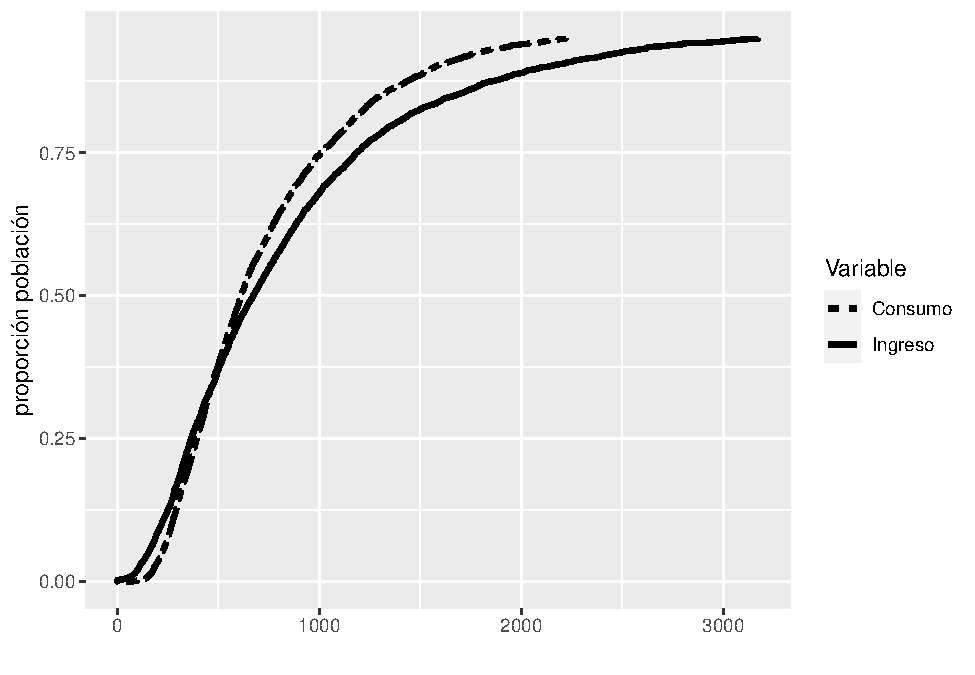
\includegraphics{_main_files/figure-latex/unnamed-chunk-64-1.pdf}

~

\hypertarget{pobreza-por-edad}{%
\section{Pobreza por edad}\label{pobreza-por-edad}}

\#\#\#- (pág. 254-255)

El bloque de código siguiente muestra cómo puede graficarse la relación entre pobreza y edad (ver figura 4.15 del texto). Para ello luego de cargar, limpiar la base y definir la línea de pobreza, generamos dos objetos \emph{``x''} e \emph{``y''} vacíos donde se almacenará los valores del eje x y el eje y. Estos valores se generaran de forma iterativa mediante un bucle que incremente secuencialmente la edad en 5 años, comenzando en 0 y terminando en 80 años. En cada vuelta estaremos generando el indicador FGT condicionando a las observaciones que caigan dentro de distintos intervalos de edad. Esto equivale a dividir a la población en grupos de edad y para cada uno de ellos calcular el indicador. Al igual que en el código anterior, el contador nos permite almacenar los valores de edad y FGT como elementos de los vectores creados inicialmente.

\begin{Shaded}
\begin{Highlighting}[]
\CommentTok{\#indico con qué base de hogares voy a trabajar}
\NormalTok{mex06 }\OtherTok{\textless{}{-}} \FunctionTok{read.dta}\NormalTok{(data\_dir }\SpecialCharTok{\%+\%} \StringTok{"Mex/2006/bases/mex06\_cedlas.dta"}\NormalTok{) }\SpecialCharTok{\%\textgreater{}\%} 
         \FunctionTok{filter}\NormalTok{(cohh}\SpecialCharTok{==}\DecValTok{1}\NormalTok{, }\SpecialCharTok{!}\FunctionTok{is.na}\NormalTok{(ipcf))}
\NormalTok{df }\OtherTok{\textless{}{-}}\NormalTok{ mex06 }

\CommentTok{\#linea de pobreza oficial}
\NormalTok{lp0}\OtherTok{=}\FloatTok{608.245}

\NormalTok{x }\OtherTok{\textless{}{-}} \FunctionTok{c}\NormalTok{()}
\NormalTok{y }\OtherTok{\textless{}{-}} \FunctionTok{c}\NormalTok{()}

\NormalTok{j}\OtherTok{=}\DecValTok{1}

\ControlFlowTok{for}\NormalTok{ (i }\ControlFlowTok{in} \FunctionTok{seq}\NormalTok{(}\DecValTok{0}\NormalTok{,}\DecValTok{80}\NormalTok{,}\AttributeTok{by=}\DecValTok{5}\NormalTok{)) \{}
  
  \FunctionTok{print}\NormalTok{(}\FunctionTok{paste}\NormalTok{(}\StringTok{"rango = ["}\NormalTok{, i, }\StringTok{","}\NormalTok{, i}\SpecialCharTok{+}\DecValTok{4}\NormalTok{, }\StringTok{"]"}\NormalTok{, }\AttributeTok{sep=}\StringTok{""}\NormalTok{))}
\NormalTok{  fgt\_edad }\OtherTok{=} \FunctionTok{FGT}\NormalTok{(}\AttributeTok{df=}\NormalTok{df, }\AttributeTok{varname=}\NormalTok{ipcf, }\AttributeTok{var\_pondera=}\NormalTok{pondera, }\AttributeTok{condicion=}\FunctionTok{paste}\NormalTok{(}\StringTok{"edad\textgreater{}="}\NormalTok{, i, }\StringTok{" \& edad\textless{}="}\NormalTok{, (i}\SpecialCharTok{+}\DecValTok{4}\NormalTok{), }\AttributeTok{sep=}\StringTok{""}\NormalTok{), }
                 \AttributeTok{alfa=}\DecValTok{0}\NormalTok{, }\AttributeTok{zeta=}\NormalTok{lp, }\AttributeTok{quiet =} \ConstantTok{TRUE}\NormalTok{)}
  
\NormalTok{  x[j]}\OtherTok{=}\NormalTok{i}
\NormalTok{  y[j]}\OtherTok{=}\NormalTok{fgt\_edad}
  
\NormalTok{  j}\OtherTok{=}\NormalTok{j}\SpecialCharTok{+}\DecValTok{1}
  
\NormalTok{\}}
\end{Highlighting}
\end{Shaded}

\begin{verbatim}
## [1] "rango = [0,4]"
## [1] "rango = [5,9]"
## [1] "rango = [10,14]"
## [1] "rango = [15,19]"
## [1] "rango = [20,24]"
## [1] "rango = [25,29]"
## [1] "rango = [30,34]"
## [1] "rango = [35,39]"
## [1] "rango = [40,44]"
## [1] "rango = [45,49]"
## [1] "rango = [50,54]"
## [1] "rango = [55,59]"
## [1] "rango = [60,64]"
## [1] "rango = [65,69]"
## [1] "rango = [70,74]"
## [1] "rango = [75,79]"
## [1] "rango = [80,84]"
\end{verbatim}

Las líneas finales grafican los resultados, superponiendo a las estimaciones de pobreza una línea de regresión polinomial de orden dos.
.

\begin{Shaded}
\begin{Highlighting}[]
\NormalTok{xst}\OtherTok{=}\NormalTok{x}\SpecialCharTok{\^{}}\DecValTok{2}
\NormalTok{aux }\OtherTok{\textless{}{-}} \FunctionTok{data.frame}\NormalTok{(x, y, xst)}

\FunctionTok{ggplot}\NormalTok{(aux, }\FunctionTok{aes}\NormalTok{(}\AttributeTok{x =}\NormalTok{ x, }\AttributeTok{y =}\NormalTok{ y)) }\SpecialCharTok{+} 
  \FunctionTok{geom\_point}\NormalTok{() }\SpecialCharTok{+} 
\FunctionTok{geom\_smooth}\NormalTok{(}\AttributeTok{method=}\NormalTok{lm, }\AttributeTok{formula =}\NormalTok{ y }\SpecialCharTok{\textasciitilde{}}\NormalTok{ x }\SpecialCharTok{+} \FunctionTok{I}\NormalTok{(x}\SpecialCharTok{\^{}}\DecValTok{2}\NormalTok{) , }\AttributeTok{colour=}\StringTok{"red"}\NormalTok{)}
\end{Highlighting}
\end{Shaded}

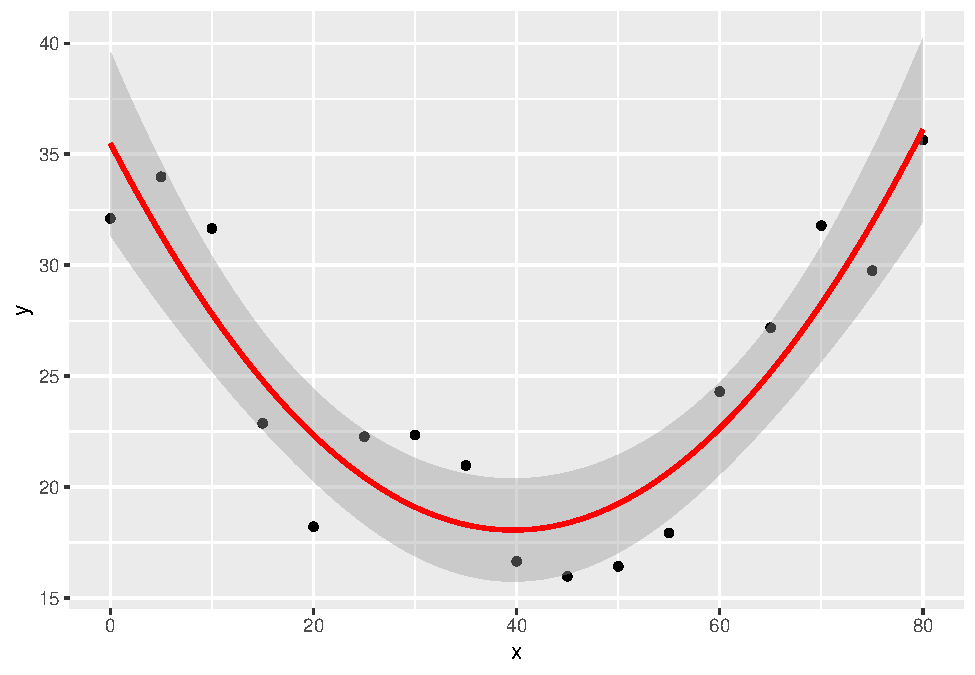
\includegraphics{_main_files/figure-latex/unnamed-chunk-66-1.pdf}

~

\hypertarget{significatividad-estadistica}{%
\section{Significatividad estadistica}\label{significatividad-estadistica}}

\#\#\#- (pág. 255-256)

En esta última sección recreamos la técnica del \emph{boostrap} o reseampleo para obtener errores estándares e intervalos de confianza para las estimaciones del FGT. La versión más simple del bootstrap requiere (i) tomar una muestra de tamaño N (el tamaño muestral) de la muestra original con reemplazo, (ii) computar el índice de pobreza deseado y (iii) repetir el procedimiento B veces, con B grande. Esto es lo que haremos mediante un bucle, fijaremos una cantidad de repeticiones, en las que en cada una estaremos tomando un resampleo de la muestra original de igual tamaño. De esta forma la muestra irá cambiando en su composición aleatoriamente y por tanto permitirá generar distintos valores del FGT en cada iteración, a partir de una misma base. El comando en R \texttt{sample\_n()} realiza esta tarea de resampleo, seteando el dataframe, el tamaño de la nueva muestra y la opción con reposición. La expresión \texttt{nrow(df)} indica que la nueva muestra tendrá el mismo tamaño que la base original. Cada valor del indicador se almacena en el objeto \emph{``store''}, sobre el que posteriormente se calcula el desvío, la media y el tamaño. Estos son inputs necesarios para la fórmula que estima los intervalos de confianza de nuestras estimaciones. En este caso estimamos un intervalo de confianza del 95\%.

\begin{Shaded}
\begin{Highlighting}[]
\NormalTok{per06 }\OtherTok{\textless{}{-}} \FunctionTok{read.dta}\NormalTok{(data\_dir }\SpecialCharTok{\%+\%} \StringTok{"Per/2006/bases/per06\_cedlas.dta"}\NormalTok{) }\SpecialCharTok{\%\textgreater{}\%} 
        \FunctionTok{filter}\NormalTok{(cohh}\SpecialCharTok{==}\DecValTok{1}\NormalTok{, }\SpecialCharTok{!}\FunctionTok{is.na}\NormalTok{(ipcf))}

\NormalTok{df }\OtherTok{\textless{}{-}}\NormalTok{ per06}

\CommentTok{\#genero un resampleo del data frame en cada iteración y para ese data frame obtengo el fgt}
\NormalTok{store }\OtherTok{\textless{}{-}} \FunctionTok{c}\NormalTok{()}
\NormalTok{rep}\OtherTok{=}\DecValTok{50}

\NormalTok{lp }\OtherTok{=} \FloatTok{128.136}

\ControlFlowTok{for}\NormalTok{ (i }\ControlFlowTok{in} \DecValTok{1}\SpecialCharTok{:}\NormalTok{rep) \{}
  
\NormalTok{   df\_sample }\OtherTok{\textless{}{-}} \FunctionTok{sample\_n}\NormalTok{(df, }\AttributeTok{size=}\FunctionTok{nrow}\NormalTok{(df), }\AttributeTok{replace=}\NormalTok{T)}
   
\NormalTok{   fgt }\OtherTok{=} \FunctionTok{FGT}\NormalTok{(}\AttributeTok{df=}\NormalTok{df\_sample, }\AttributeTok{varname=}\NormalTok{ipcf, }\AttributeTok{var\_pondera=}\NormalTok{pondera, }\AttributeTok{alfa=}\DecValTok{0}\NormalTok{, }\AttributeTok{zeta=}\NormalTok{lp, }\AttributeTok{quiet =} \ConstantTok{TRUE}\NormalTok{)}
\NormalTok{   store[i] }\OtherTok{=}\NormalTok{ fgt}
   
\NormalTok{\}}
\end{Highlighting}
\end{Shaded}

\begin{Shaded}
\begin{Highlighting}[]
\NormalTok{store}
\end{Highlighting}
\end{Shaded}

\begin{verbatim}
##  [1] 25.29 25.12 25.30 25.25 25.55 25.25 25.54 25.36 25.41 25.23 25.13 25.01
## [13] 25.44 25.42 25.13 24.85 24.88 25.29 25.42 25.26 25.42 25.24 25.19 25.11
## [25] 25.34 25.15 24.98 25.30 25.47 25.37 25.21 25.50 24.99 25.34 25.50 25.11
## [37] 24.98 25.51 25.30 25.26 25.50 25.37 25.16 25.04 25.40 25.58 25.12 25.40
## [49] 25.39 24.88
\end{verbatim}

\begin{Shaded}
\begin{Highlighting}[]
\NormalTok{sd}\OtherTok{=}\FunctionTok{sd}\NormalTok{(store)}
\NormalTok{mean}\OtherTok{=}\FunctionTok{mean}\NormalTok{(store)}
\NormalTok{n}\OtherTok{=}\FunctionTok{length}\NormalTok{(store)}

\CommentTok{\#con intervalo de confianza del 95\%}
\NormalTok{error }\OtherTok{\textless{}{-}} \FunctionTok{qt}\NormalTok{(}\FloatTok{0.975}\NormalTok{,}\AttributeTok{df=}\NormalTok{n}\DecValTok{{-}1}\NormalTok{)}\SpecialCharTok{*}\NormalTok{sd}\SpecialCharTok{/}\FunctionTok{sqrt}\NormalTok{(n)}
\NormalTok{left }\OtherTok{\textless{}{-}}\NormalTok{ mean }\SpecialCharTok{{-}}\NormalTok{ error; left}
\end{Highlighting}
\end{Shaded}

\begin{verbatim}
## [1] 25.21138
\end{verbatim}

\begin{Shaded}
\begin{Highlighting}[]
\NormalTok{right }\OtherTok{\textless{}{-}}\NormalTok{ mean }\SpecialCharTok{+}\NormalTok{ error; right}
\end{Highlighting}
\end{Shaded}

\begin{verbatim}
## [1] 25.31822
\end{verbatim}

A modo de extensión es fácil escribir una función que, tomando los resultados alojados en un vector y el intervalo de confianza deseado, nos devuelve directamente el cálculo del intervalo.

\begin{Shaded}
\begin{Highlighting}[]
\CommentTok{\#también es posible hacer un función para calcular los intervalos de confianza}
\NormalTok{ci }\OtherTok{\textless{}{-}} \ControlFlowTok{function}\NormalTok{(vector, intervalo)\{}
  
\NormalTok{  sd}\OtherTok{=}\FunctionTok{sd}\NormalTok{(vector)}
\NormalTok{  mean}\OtherTok{=}\FunctionTok{mean}\NormalTok{(vector)}
\NormalTok{  n}\OtherTok{=} \FunctionTok{length}\NormalTok{(vector)}
  
\NormalTok{  error }\OtherTok{\textless{}{-}} \FunctionTok{qt}\NormalTok{((intervalo}\SpecialCharTok{+}\DecValTok{1}\NormalTok{)}\SpecialCharTok{/}\DecValTok{2}\NormalTok{, }\AttributeTok{df=}\NormalTok{n}\DecValTok{{-}1}\NormalTok{) }\SpecialCharTok{*}\NormalTok{ sd}\SpecialCharTok{/}\FunctionTok{sqrt}\NormalTok{(n)}
\NormalTok{  result }\OtherTok{\textless{}{-}} \FunctionTok{c}\NormalTok{(}\StringTok{"lower"} \OtherTok{=}\NormalTok{ mean }\SpecialCharTok{{-}}\NormalTok{ error, }\StringTok{"upper"} \OtherTok{=}\NormalTok{ mean }\SpecialCharTok{+}\NormalTok{ error)}
  \FunctionTok{return}\NormalTok{(result)}
\NormalTok{\}}
\end{Highlighting}
\end{Shaded}

\begin{Shaded}
\begin{Highlighting}[]
\FunctionTok{ci}\NormalTok{(store, }\FloatTok{0.90}\NormalTok{)}
\end{Highlighting}
\end{Shaded}

\begin{verbatim}
##    lower    upper 
## 25.22024 25.30936
\end{verbatim}

\begin{Shaded}
\begin{Highlighting}[]
\FunctionTok{ci}\NormalTok{(store, }\FloatTok{0.95}\NormalTok{)}
\end{Highlighting}
\end{Shaded}

\begin{verbatim}
##    lower    upper 
## 25.21138 25.31822
\end{verbatim}

\begin{Shaded}
\begin{Highlighting}[]
\FunctionTok{ci}\NormalTok{(store, }\FloatTok{0.99}\NormalTok{)}
\end{Highlighting}
\end{Shaded}

\begin{verbatim}
##    lower    upper 
## 25.19356 25.33604
\end{verbatim}

\hypertarget{capuxedtulo-5}{%
\chapter{Capítulo 5}\label{capuxedtulo-5}}

\hypertarget{pobreza-extensiones}{%
\section*{Pobreza: extensiones}\label{pobreza-extensiones}}

\hypertarget{escrito-por-cristian-bonavida-3}{%
\subsubsection*{Escrito por: Cristian Bonavida}\label{escrito-por-cristian-bonavida-3}}
\addcontentsline{toc}{subsubsection}{Escrito por: Cristian Bonavida}

\hypertarget{last-update-0272021-2}{%
\subsubsection*{Last Update: 02/7/2021}\label{last-update-0272021-2}}
\addcontentsline{toc}{subsubsection}{Last Update: 02/7/2021}

~

\emph{Códigos escritos en base a los apéndices del libro ``Pobreza y Desigualdad en América Latina'' de Gasparini, Cicowiez y Sosa Escudero. El objeto de este material es reproducir la rutina de códigos para STATA presentada en el libro al lenguaje R. Este material es solo de caracter complementario a las explicaciones y detalles conceptuales que se presentan en el libro de texto y los apéndices}

~

\hypertarget{set-inicial-3}{%
\section*{Set Inicial}\label{set-inicial-3}}
\addcontentsline{toc}{section}{Set Inicial}

Cargo las librerias, limpio enviroment, defino el path y atajo para funcion paste

\begin{Shaded}
\begin{Highlighting}[]
\FunctionTok{library}\NormalTok{(dplyr)}
\FunctionTok{library}\NormalTok{(tidyverse) }\CommentTok{\# Data wrangling}
\FunctionTok{library}\NormalTok{(tidygraph)}
\FunctionTok{library}\NormalTok{(readxl)}
\FunctionTok{library}\NormalTok{(ggplot2)}
\FunctionTok{library}\NormalTok{(foreign)}
\FunctionTok{library}\NormalTok{(TAM)}
\FunctionTok{library}\NormalTok{(margins)}

\FunctionTok{rm}\NormalTok{(}\AttributeTok{list=}\FunctionTok{ls}\NormalTok{())    }\CommentTok{\#empiezo limpiando todo }

\StringTok{"\%+\%"} \OtherTok{\textless{}{-}} \ControlFlowTok{function}\NormalTok{(x,y) }\FunctionTok{paste}\NormalTok{(x,y,}\AttributeTok{sep =} \StringTok{""}\NormalTok{)      }\CommentTok{\# defino un shorcut parar concat de texto}
\NormalTok{data\_dir }\OtherTok{\textless{}{-}} \StringTok{"C:/Users/HP/Desktop/CEDLAS {-} UNLP/Apendices en R/Material libro/encuestas{-}cedlas/Encuestas/"}  \CommentTok{\#seteo directorio }
\end{Highlighting}
\end{Shaded}

~

\hypertarget{pobreza-multidimensional}{%
\section{Pobreza Multidimensional}\label{pobreza-multidimensional}}

\#\#\#- (pág. 334-335)

En este primer apartado se muestra cómo puede replicarse el cuadro 5.1 del libro, sobre tasas de pobreza multidimensional en Nicaragua, Perú y Uruguay. Comenzamos cargando y defiendo la base a utilizar

\begin{Shaded}
\begin{Highlighting}[]
\NormalTok{nic05 }\OtherTok{\textless{}{-}} \FunctionTok{read.dta}\NormalTok{(data\_dir }\SpecialCharTok{\%+\%} \StringTok{"Nic/2005/bases/nic05\_cedlas.dta"}\NormalTok{)      }
\NormalTok{df }\OtherTok{\textless{}{-}}\NormalTok{ nic05}
\end{Highlighting}
\end{Shaded}

Nos asegurarnos de convertir los missings que puede contener la variable pondera a 0. De esta manera al calcular estimadores ponderados los valores para estas observaciones no tienen ningun peso y evitamos que los missings afecten el nuestros cálculos.

\begin{Shaded}
\begin{Highlighting}[]
\NormalTok{df}\SpecialCharTok{$}\NormalTok{pondera }\OtherTok{\textless{}{-}} \FunctionTok{ifelse}\NormalTok{(}\FunctionTok{is.na}\NormalTok{(df}\SpecialCharTok{$}\NormalTok{pondera), }\DecValTok{0}\NormalTok{, df}\SpecialCharTok{$}\NormalTok{pondera)}
\end{Highlighting}
\end{Shaded}

El bloque de código siguiente asigna a todos los miembros del hogar las variables que solo están definidas para el jefe de hogar. Como se trata de variables relacionadas con las características de la vivienda, típicamente se encuentran en las bases de datos de hogares y no de personas.

En STATA la solución se propone con un bucle. En este caso aplicamos la misma lógica pero nos valemos de la función \texttt{across} que nos permite realizar un mismo cálculo para un conjunto de columnas especificadas. Previamente debemos ordenar y agrupar las observaciones por id.

\begin{Shaded}
\begin{Highlighting}[]
\NormalTok{df }\OtherTok{\textless{}{-}}\NormalTok{ df }\SpecialCharTok{\%\textgreater{}\%} \FunctionTok{arrange}\NormalTok{(id) }\SpecialCharTok{\%\textgreater{}\%} \FunctionTok{group\_by}\NormalTok{(id) }\SpecialCharTok{\%\textgreater{}\%}
      \FunctionTok{mutate}\NormalTok{(}
        \FunctionTok{across}\NormalTok{(}
         \AttributeTok{.cols  =} \FunctionTok{c}\NormalTok{(habita, matpreca, agua, banio), }\CommentTok{\#sobre qué columnas aplicar operación}
         \AttributeTok{.fns   =}\NormalTok{ mean,   }\CommentTok{\#que operación/función queremos realizar}
          \AttributeTok{na.rm =} \ConstantTok{TRUE}\NormalTok{,                                 }
         \AttributeTok{.names =} \StringTok{"\{col\}"} \CommentTok{\#como deben llamarse las nuevas variables}
\NormalTok{                )}
\NormalTok{                  )}
\end{Highlighting}
\end{Shaded}

La expresión \texttt{names\ =\ "\{col\}"} indica que el nombre de las nuevas columnas sea el nombre de las variables orginales, por lo que las estamos sobreescribiendo.

En las siguiente bloque de código calculamos los indicadores de pobreza para cada una de las dimensiones relevantes, creando un nueva variable en el data frame para cada caso. Empleamos el comando \texttt{ifelse} cuando el cálculo es directo y \texttt{mutate} cuando se requiere de una variable auxiliar previa.

\begin{Shaded}
\begin{Highlighting}[]
\CommentTok{\# (1) ipcf \textless{} 2.5 USD}
\NormalTok{df}\SpecialCharTok{$}\NormalTok{indic1 }\OtherTok{\textless{}{-}} \FunctionTok{ifelse}\NormalTok{(df}\SpecialCharTok{$}\NormalTok{ipcf }\SpecialCharTok{\textless{}} \FloatTok{564.12}\NormalTok{, }\DecValTok{1}\NormalTok{ ,}\DecValTok{0}\NormalTok{)}

\CommentTok{\# (2) mas de 3 miembros por cuarto}
\NormalTok{df }\OtherTok{\textless{}{-}}\NormalTok{ df }\SpecialCharTok{\%\textgreater{}\%} \FunctionTok{mutate}\NormalTok{(}
              \AttributeTok{rat\_miembros\_cuartos =}\NormalTok{ miembros}\SpecialCharTok{/}\NormalTok{habita,}
              \AttributeTok{aux =} \FunctionTok{case\_when}\NormalTok{(}
\NormalTok{                    (rat\_miembros\_cuartos}\SpecialCharTok{\textgreater{}}\DecValTok{3} \SpecialCharTok{\&} \SpecialCharTok{!}\FunctionTok{is.na}\NormalTok{(rat\_miembros\_cuartos)) }\SpecialCharTok{\textasciitilde{}} \DecValTok{1}\NormalTok{, }
\NormalTok{                    (rat\_miembros\_cuartos}\SpecialCharTok{\textless{}=}\DecValTok{3} \SpecialCharTok{\&} \SpecialCharTok{!}\FunctionTok{is.na}\NormalTok{(rat\_miembros\_cuartos)) }\SpecialCharTok{\textasciitilde{}} \DecValTok{0}\NormalTok{)) }\SpecialCharTok{\%\textgreater{}\%}
             \FunctionTok{group\_by}\NormalTok{(id) }\SpecialCharTok{\%\textgreater{}\%} \FunctionTok{mutate}\NormalTok{(}\AttributeTok{indic2=}\FunctionTok{max}\NormalTok{(aux)) }\SpecialCharTok{\%\textgreater{}\%} \FunctionTok{select}\NormalTok{(}\SpecialCharTok{{-}}\NormalTok{aux)}

\CommentTok{\# (3) vivienda construida con material precario}
\NormalTok{df}\SpecialCharTok{$}\NormalTok{indic3 }\OtherTok{\textless{}{-}} \FunctionTok{ifelse}\NormalTok{(df}\SpecialCharTok{$}\NormalTok{matpreca}\SpecialCharTok{==}\DecValTok{1}\NormalTok{, }\DecValTok{1}\NormalTok{ ,}\DecValTok{0}\NormalTok{)}

\CommentTok{\# (4) vivienda sin acceso a agua potable}
\NormalTok{df}\SpecialCharTok{$}\NormalTok{indic4 }\OtherTok{\textless{}{-}} \FunctionTok{ifelse}\NormalTok{(df}\SpecialCharTok{$}\NormalTok{agua}\SpecialCharTok{==}\DecValTok{0}\NormalTok{, }\DecValTok{1}\NormalTok{ ,}\DecValTok{0}\NormalTok{)}

\CommentTok{\# (5) vivienda sin acceso a baño sanitario }
\NormalTok{df}\SpecialCharTok{$}\NormalTok{indic5 }\OtherTok{\textless{}{-}} \FunctionTok{ifelse}\NormalTok{(df}\SpecialCharTok{$}\NormalTok{banio}\SpecialCharTok{==}\DecValTok{0}\NormalTok{, }\DecValTok{1}\NormalTok{ ,}\DecValTok{0}\NormalTok{)}

\CommentTok{\# (6) educación promedio menor a 7 años solo para el jefe y conyuge}
\NormalTok{df }\OtherTok{\textless{}{-}}\NormalTok{ df }\SpecialCharTok{\%\textgreater{}\%} \FunctionTok{mutate}\NormalTok{(}\AttributeTok{aedu\_avg =} \FunctionTok{ifelse}\NormalTok{(jefe}\SpecialCharTok{==}\DecValTok{1} \SpecialCharTok{|}\NormalTok{ conyuge}\SpecialCharTok{==}\DecValTok{1}\NormalTok{, }\FunctionTok{mean}\NormalTok{(aedu, }\AttributeTok{na.rm=}\ConstantTok{TRUE}\NormalTok{), }\ConstantTok{NA}\NormalTok{),}
                    \AttributeTok{aux =} \FunctionTok{ifelse}\NormalTok{(aedu\_avg}\SpecialCharTok{\textless{}}\DecValTok{7} \SpecialCharTok{\&}\NormalTok{ jefe}\SpecialCharTok{==}\DecValTok{1}\NormalTok{, }\DecValTok{1}\NormalTok{ ,}\DecValTok{0}\NormalTok{)) }\SpecialCharTok{\%\textgreater{}\%} \FunctionTok{group\_by}\NormalTok{(id) }\SpecialCharTok{\%\textgreater{}\%}
             \FunctionTok{mutate}\NormalTok{(}\AttributeTok{indic6 =} \FunctionTok{max}\NormalTok{(aux))  }\SpecialCharTok{\%\textgreater{}\%} \FunctionTok{select}\NormalTok{(}\SpecialCharTok{{-}}\NormalTok{aux)}
\end{Highlighting}
\end{Shaded}

Seguidamente obtenemos el porcentaje de personas con privaciones para cada indicador, utilizando la media ponderada.

\begin{Shaded}
\begin{Highlighting}[]
\FunctionTok{weighted.mean}\NormalTok{(df}\SpecialCharTok{$}\NormalTok{indic1, df}\SpecialCharTok{$}\NormalTok{pondera, }\AttributeTok{na.rm=}\ConstantTok{TRUE}\NormalTok{)}\SpecialCharTok{*}\DecValTok{100}
\end{Highlighting}
\end{Shaded}

\begin{verbatim}
## [1] 42.66527
\end{verbatim}

\begin{Shaded}
\begin{Highlighting}[]
\FunctionTok{weighted.mean}\NormalTok{(df}\SpecialCharTok{$}\NormalTok{indic2, df}\SpecialCharTok{$}\NormalTok{pondera, }\AttributeTok{na.rm=}\ConstantTok{TRUE}\NormalTok{)}\SpecialCharTok{*}\DecValTok{100}
\end{Highlighting}
\end{Shaded}

\begin{verbatim}
## [1] 35.15812
\end{verbatim}

\begin{Shaded}
\begin{Highlighting}[]
\FunctionTok{weighted.mean}\NormalTok{(df}\SpecialCharTok{$}\NormalTok{indic3, df}\SpecialCharTok{$}\NormalTok{pondera, }\AttributeTok{na.rm=}\ConstantTok{TRUE}\NormalTok{)}\SpecialCharTok{*}\DecValTok{100}
\end{Highlighting}
\end{Shaded}

\begin{verbatim}
## [1] 14.43805
\end{verbatim}

\begin{Shaded}
\begin{Highlighting}[]
\FunctionTok{weighted.mean}\NormalTok{(df}\SpecialCharTok{$}\NormalTok{indic4, df}\SpecialCharTok{$}\NormalTok{pondera, }\AttributeTok{na.rm=}\ConstantTok{TRUE}\NormalTok{)}\SpecialCharTok{*}\DecValTok{100}
\end{Highlighting}
\end{Shaded}

\begin{verbatim}
## [1] 37.31393
\end{verbatim}

\begin{Shaded}
\begin{Highlighting}[]
\FunctionTok{weighted.mean}\NormalTok{(df}\SpecialCharTok{$}\NormalTok{indic5, df}\SpecialCharTok{$}\NormalTok{pondera, }\AttributeTok{na.rm=}\ConstantTok{TRUE}\NormalTok{)}\SpecialCharTok{*}\DecValTok{100}
\end{Highlighting}
\end{Shaded}

\begin{verbatim}
## [1] 73.09805
\end{verbatim}

\begin{Shaded}
\begin{Highlighting}[]
\FunctionTok{weighted.mean}\NormalTok{(df}\SpecialCharTok{$}\NormalTok{indic6, df}\SpecialCharTok{$}\NormalTok{pondera, }\AttributeTok{na.rm=}\ConstantTok{TRUE}\NormalTok{)}\SpecialCharTok{*}\DecValTok{100}
\end{Highlighting}
\end{Shaded}

\begin{verbatim}
## [1] 73.3585
\end{verbatim}

La variable ``npriv'' contiene el número de privaciones de cada individuo. Para crearla utilizamos una operación a nivel de fila con el comando \texttt{rowSums} que, combinado con \texttt{across}, nos permite sumar todas las columnas especificadas. En este caso especificamos todas las columnas que comienzan con el patron ``indic''. Notese que a diferencia del uso anterior aqui no se realiza una misma operación repetida para cada columna sino que se especifican las columnas que se incluyen como argumento de la operación suma.

\begin{Shaded}
\begin{Highlighting}[]
\CommentTok{\#contar condiciones:por fila sumo todas las columnas que comienzan con indic}
\NormalTok{df }\OtherTok{\textless{}{-}}\NormalTok{ df }\SpecialCharTok{\%\textgreater{}\%} \FunctionTok{mutate}\NormalTok{(}\AttributeTok{npriv =} \FunctionTok{rowSums}\NormalTok{(}\FunctionTok{across}\NormalTok{(}\FunctionTok{starts\_with}\NormalTok{(}\StringTok{"indic"}\NormalTok{)))) }
\end{Highlighting}
\end{Shaded}

Una forma alternativa más intuitiva sería especificar manualmente las columnas a sumar, pero se vuelve poco efeciente en el caso de que estas sean numerosas, por lo que la posibilidad de identificar columnas por patrones se vuelve particularmente atractiva.

\begin{Shaded}
\begin{Highlighting}[]
\CommentTok{\#manera alternativa}
\NormalTok{df}\SpecialCharTok{$}\NormalTok{npriv }\OtherTok{=}\NormalTok{ df}\SpecialCharTok{$}\NormalTok{indic1 }\SpecialCharTok{+}\NormalTok{ df}\SpecialCharTok{$}\NormalTok{indic2 }\SpecialCharTok{+}\NormalTok{ df}\SpecialCharTok{$}\NormalTok{indic3 }\SpecialCharTok{+}\NormalTok{ df}\SpecialCharTok{$}\NormalTok{indic4 }\SpecialCharTok{+}\NormalTok{ df}\SpecialCharTok{$}\NormalTok{indic5 }\SpecialCharTok{+}\NormalTok{ df}\SpecialCharTok{$}\NormalTok{indic6   }
\end{Highlighting}
\end{Shaded}

A partir de la variable ``npriv'' se generan las variables ``pobre1'' a ``pobre6'' que valen 1 de acuerdo con la cantidad de privaciones que sufre cada individuo. Por ejemplo, la variable ``pobre4'' vale 1 para los individuos que tienen 4 o más privaciones, y 0 en caso contrario.

En cada iteración se concatena el prefijo \emph{pobre} con el contador \texttt{i}, dandole nombre a cada nueva columna del data frame. Luego se calcula el porcentaje como la media ponderada de esta columna, se redondea e imprime el resultado.

\begin{Shaded}
\begin{Highlighting}[]
\CommentTok{\#condición de pobreza segun cantidad de privaciones}
\ControlFlowTok{for}\NormalTok{ (i }\ControlFlowTok{in} \DecValTok{1}\SpecialCharTok{:}\DecValTok{6}\NormalTok{)\{}
  
\NormalTok{  df[}\FunctionTok{paste}\NormalTok{(}\StringTok{"pobre"}\NormalTok{,i,}\AttributeTok{sep=}\StringTok{""}\NormalTok{)] }\OtherTok{\textless{}{-}} \FunctionTok{ifelse}\NormalTok{(df}\SpecialCharTok{$}\NormalTok{npriv}\SpecialCharTok{\textgreater{}=}\NormalTok{i, }\DecValTok{1}\NormalTok{, }\DecValTok{0}\NormalTok{)}
  
\NormalTok{  p }\OtherTok{=} \FunctionTok{weighted.mean}\NormalTok{(df[}\FunctionTok{paste}\NormalTok{(}\StringTok{"pobre"}\NormalTok{,i,}\AttributeTok{sep=}\StringTok{""}\NormalTok{)], df[}\StringTok{"pondera"}\NormalTok{], }\AttributeTok{na.rm=}\ConstantTok{TRUE}\NormalTok{)}\SpecialCharTok{*}\DecValTok{100}
  \FunctionTok{print}\NormalTok{(}\FunctionTok{paste}\NormalTok{(i, }\StringTok{" privaciones = "}\NormalTok{, }\FunctionTok{round}\NormalTok{(p, }\AttributeTok{d=}\DecValTok{2}\NormalTok{), }\StringTok{"\%"}\NormalTok{, }\AttributeTok{sep =} \StringTok{""}\NormalTok{))}
  
\NormalTok{\}}
\end{Highlighting}
\end{Shaded}

\begin{verbatim}
## [1] "1 privaciones = 86.75%"
## [1] "2 privaciones = 73.02%"
## [1] "3 privaciones = 56.6%"
## [1] "4 privaciones = 37.67%"
## [1] "5 privaciones = 19.2%"
## [1] "6 privaciones = 4.51%"
\end{verbatim}

~

\hypertarget{indice-bourguignon-y-chakravarty-bc---pobreza-multidimensional}{%
\section{Indice Bourguignon y Chakravarty (BC) - Pobreza Multidimensional}\label{indice-bourguignon-y-chakravarty-bc---pobreza-multidimensional}}

\#\#\#- (pág. 335-336)

El código a continuación permite reproducir el cuadro 5.2 del texto sobre pobreza multidimensional computada con el índice de Bourguignon y Chakravarty (BC). El cómputo de dicho índice se realiza empleando solo las observaciones que tienen información para las tres dimensiones consideradas en el texto; por lo que se eliminan las observaciones con missing en al menos una de esas dimensiones. Se eligen los valores para los parametros relevantes y se fija el número de dimensiones a considerar

\begin{Shaded}
\begin{Highlighting}[]
\NormalTok{df }\OtherTok{\textless{}{-}}\NormalTok{ df }\SpecialCharTok{\%\textgreater{}\%} \FunctionTok{filter}\NormalTok{(}\SpecialCharTok{!}\FunctionTok{is.na}\NormalTok{(ipcf), }\SpecialCharTok{!}\FunctionTok{is.na}\NormalTok{(aedu\_avg), }\SpecialCharTok{!}\FunctionTok{is.na}\NormalTok{(rat\_miembros\_cuartos))}

\NormalTok{theta}\OtherTok{=}\DecValTok{1}  
\NormalTok{alpha}\OtherTok{=}\DecValTok{2}

\NormalTok{dim\_t}\OtherTok{=}\DecValTok{3}    \CommentTok{\#total dimensiones}
\end{Highlighting}
\end{Shaded}

Posteriormente almacenamos los valores de las observacion en una lista, donde cada elemento contiene todos los valores de cada una de las 3 variables a considerar. En vectores separados almacenamos los umbrales y los pesos

\begin{Shaded}
\begin{Highlighting}[]
\NormalTok{dimension }\OtherTok{\textless{}{-}} \FunctionTok{list}\NormalTok{( df}\SpecialCharTok{$}\NormalTok{ipcf,                  }\CommentTok{\# (1) ipcf }
             \DecValTok{1}\SpecialCharTok{/}\NormalTok{df}\SpecialCharTok{$}\NormalTok{rat\_miembros\_cuartos,      }\CommentTok{\# (2) ratio de miembros por cuarto}
\NormalTok{             df}\SpecialCharTok{$}\NormalTok{aedu\_avg                     }\CommentTok{\# (3) educación promedio de jefe y conyuge}
\NormalTok{              )}

\NormalTok{umbral }\OtherTok{\textless{}{-}} \FunctionTok{c}\NormalTok{(}\FloatTok{564.119195}\NormalTok{, }\DecValTok{1}\SpecialCharTok{/}\DecValTok{3}\NormalTok{, }\DecValTok{7}\NormalTok{)   }\CommentTok{\#valores para los umbrales de cada dimensiones}
\NormalTok{wt }\OtherTok{\textless{}{-}} \FunctionTok{c}\NormalTok{(}\DecValTok{1}\NormalTok{, }\DecValTok{1}\NormalTok{, }\DecValTok{1}\NormalTok{)                  }\CommentTok{\#wt correspondiente}
\end{Highlighting}
\end{Shaded}

El objeto brechas se define como vacío y cada uno de sus elementos se genera en las iteraciones sucesivas del bucle al comparar cada valor de la variable contra los umbrales fijados. El objeto ``suma\_brechas'' se crea como un vector único con valores 0, y luego se reemplaza iterativamente para computar la suma de brechas. El bucle itera \emph{n} veces en total, siendo \emph{n} la cantidad de dimensiones relevadas. En cada iteracion replica la formula de BC para cada dimensión.

\begin{Shaded}
\begin{Highlighting}[]
\CommentTok{\#defino la lista brechas como vacia para generar cada uno de sus elementos en el bucle}
\NormalTok{brecha }\OtherTok{\textless{}{-}} \FunctionTok{list}\NormalTok{()}

\NormalTok{suma\_brechas }\OtherTok{\textless{}{-}} \FunctionTok{c}\NormalTok{(}\FunctionTok{rep}\NormalTok{(}\DecValTok{0}\NormalTok{, }\FunctionTok{nrow}\NormalTok{(df)))}

\ControlFlowTok{for}\NormalTok{ (i }\ControlFlowTok{in} \DecValTok{1}\SpecialCharTok{:}\NormalTok{dim\_t) \{}
  
  \CommentTok{\#generar brechas a partir de valores de las dimensiones vs umbrales}
\NormalTok{  brecha[[i]] }\OtherTok{\textless{}{-}} \FunctionTok{ifelse}\NormalTok{(dimension[[i]]}\SpecialCharTok{\textless{}}\NormalTok{umbral[i], }\DecValTok{1}\SpecialCharTok{{-}}\NormalTok{dimension[[i]]}\SpecialCharTok{/}\NormalTok{umbral[i], }\DecValTok{0}\NormalTok{)}
  
  \CommentTok{\#construir brechas ponderadas}
\NormalTok{  brecha[[i]] }\OtherTok{\textless{}{-}}\NormalTok{ wt[i]}\SpecialCharTok{/}\NormalTok{dim\_t }\SpecialCharTok{*}\NormalTok{ (brecha[[i]]}\SpecialCharTok{\^{}}\NormalTok{theta)}
  
  \CommentTok{\#computar suma de las brechas. Suma\_brechas será = 0 solo si todas las brechas son 0}
\NormalTok{  suma\_brechas }\OtherTok{=}\NormalTok{ suma\_brechas }\SpecialCharTok{+}\NormalTok{ brecha[[i]]}
  
\NormalTok{\}}
\end{Highlighting}
\end{Shaded}

Finalmente se calcula, para cada individuo, la suma de las brechas ponderadas elevadas a la potencia \emph{theta}, siempre que la suma de las brechas sea distinta de cero. Por último, se computa el índice BC como el cociente entre la suma ponderada de las brechas individuales almacenadas en la variable suma\_brechas y la población de referencia.

\begin{Shaded}
\begin{Highlighting}[]
\NormalTok{suma\_brechas }\OtherTok{=} \FunctionTok{ifelse}\NormalTok{(suma\_brechas}\SpecialCharTok{!=}\DecValTok{0}\NormalTok{, suma\_brechas}\SpecialCharTok{\^{}}\NormalTok{(alpha}\SpecialCharTok{/}\NormalTok{theta), suma\_brechas)}
                      
\NormalTok{BC }\OtherTok{=} \FunctionTok{round}\NormalTok{(}\FunctionTok{sum}\NormalTok{(suma\_brechas}\SpecialCharTok{*}\NormalTok{df}\SpecialCharTok{$}\NormalTok{pondera)}\SpecialCharTok{/}\FunctionTok{sum}\NormalTok{(df}\SpecialCharTok{$}\NormalTok{pondera), }\AttributeTok{d=}\DecValTok{3}\NormalTok{)}

\FunctionTok{print}\NormalTok{(}\FunctionTok{paste}\NormalTok{(}\StringTok{"BC ="}\NormalTok{, BC))}
\end{Highlighting}
\end{Shaded}

\begin{verbatim}
## [1] "BC = 0.08"
\end{verbatim}

~

\hypertarget{indice-alkire-y-foster-af---pobreza-multidimensional}{%
\section{Indice Alkire y Foster (AF) - Pobreza Multidimensional}\label{indice-alkire-y-foster-af---pobreza-multidimensional}}

\#\#\#- (pág. 337-338)

A continuación se replica la formula de Alkire y Foster que permite replicar el cuadro 5.3 del texto. Las primeras lineas son identicas al caso anterior, cambiando los parametros de interés y agregando la lista ``pobre'' como objeto vacío.

\begin{Shaded}
\begin{Highlighting}[]
\NormalTok{k}\OtherTok{=}\DecValTok{2}
\NormalTok{alpha}\OtherTok{=}\DecValTok{2}

\NormalTok{dim\_t}\OtherTok{=}\DecValTok{3}

\NormalTok{dim }\OtherTok{\textless{}{-}} \FunctionTok{list}\NormalTok{( df}\SpecialCharTok{$}\NormalTok{ipcf,                       }
             \DecValTok{1}\SpecialCharTok{/}\NormalTok{df}\SpecialCharTok{$}\NormalTok{rat\_miembros\_cuartos,      }
\NormalTok{             df}\SpecialCharTok{$}\NormalTok{aedu\_avg                     }
\NormalTok{)}

\NormalTok{umbral }\OtherTok{\textless{}{-}} \FunctionTok{c}\NormalTok{(}\FloatTok{564.119195}\NormalTok{, }\DecValTok{1}\SpecialCharTok{/}\DecValTok{3}\NormalTok{, }\DecValTok{7}\NormalTok{)}
\NormalTok{wt }\OtherTok{\textless{}{-}} \FunctionTok{c}\NormalTok{(}\DecValTok{1}\NormalTok{, }\DecValTok{1}\NormalTok{, }\DecValTok{1}\NormalTok{)}

\CommentTok{\#defino la lista "brechas" Y pobre como vacia para generar cada uno de sus elementos en el bucle}
\NormalTok{brecha }\OtherTok{\textless{}{-}} \FunctionTok{list}\NormalTok{()}
\NormalTok{pobre }\OtherTok{\textless{}{-}} \FunctionTok{list}\NormalTok{()}
\end{Highlighting}
\end{Shaded}

Nuevamente el bucle itera sobre las \emph{n} dimensiones fijada generando los valores de brecha para cada observación y ahora también completando el objeto binario ``pobre'' según el valor que toma la brecha. Al finalizar el bucle se construye el objeto ``npriv'' que contiene el número de dimensiones en que cada individuo fue identificado como pobre (vale cero para los individuos no pobres). El objeto ``pobre\_k'' vale 1 para los individuos que son pobres en, al menos, k dimensiones.

\begin{Shaded}
\begin{Highlighting}[]
\ControlFlowTok{for}\NormalTok{ (i }\ControlFlowTok{in} \DecValTok{1}\SpecialCharTok{:}\NormalTok{dim\_t) \{}
  
    \CommentTok{\#generar brechas a partir de valores de las dimensiones vs umbrales}
\NormalTok{    brecha[[i]] }\OtherTok{\textless{}{-}} \FunctionTok{ifelse}\NormalTok{(dim[[i]]}\SpecialCharTok{\textless{}}\NormalTok{umbral[i], (}\DecValTok{1}\SpecialCharTok{{-}}\NormalTok{dim[[i]]}\SpecialCharTok{/}\NormalTok{umbral[i])}\SpecialCharTok{\^{}}\NormalTok{alpha, }\DecValTok{0}\NormalTok{)}
    
    \CommentTok{\#identificar si es pobre en dimensión i}
\NormalTok{    pobre[[i]] }\OtherTok{\textless{}{-}} \FunctionTok{ifelse}\NormalTok{(brecha[[i]]}\SpecialCharTok{!=}\DecValTok{0}\NormalTok{, }\DecValTok{1}\NormalTok{, }\DecValTok{0}\NormalTok{)}
  
\NormalTok{  \}}


\CommentTok{\#identificar pobres en al menos k dimensiones}
\NormalTok{npriv }\OtherTok{=}\NormalTok{ pobre[[}\DecValTok{1}\NormalTok{]] }\SpecialCharTok{+}\NormalTok{ pobre[[}\DecValTok{2}\NormalTok{]] }\SpecialCharTok{+}\NormalTok{ pobre[[}\DecValTok{3}\NormalTok{]]}
\NormalTok{pobre\_k }\OtherTok{=} \FunctionTok{ifelse}\NormalTok{(npriv}\SpecialCharTok{\textgreater{}=}\NormalTok{k, }\DecValTok{1}\NormalTok{, }\DecValTok{0}\NormalTok{)}
\end{Highlighting}
\end{Shaded}

La línea siguiente genera la variable ``suma\_brechas'' que, como antes, se emplea luego para almacenar la suma de las brechas en cada una de las dimensiones consideradas. El bucle constuye para cada dimensión los objetos necesarios para replicar la formula de AK

\begin{Shaded}
\begin{Highlighting}[]
\ControlFlowTok{for}\NormalTok{ (i }\ControlFlowTok{in} \DecValTok{1}\SpecialCharTok{:}\NormalTok{dim\_t) \{  }
  
    \CommentTok{\#brechas positivas solo si el número de privaciones mayor a k}
\NormalTok{    brecha[[i]] }\OtherTok{\textless{}{-}} \FunctionTok{ifelse}\NormalTok{(pobre\_k}\SpecialCharTok{!=}\DecValTok{1}\NormalTok{, }\DecValTok{0}\NormalTok{, brecha[[i]])}
    
    \CommentTok{\#construir brechas ponderadas}
\NormalTok{    brecha[[i]] }\OtherTok{\textless{}{-}}\NormalTok{ wt[i] }\SpecialCharTok{*}\NormalTok{ brecha[[i]]}
    
    \CommentTok{\#computar suma de las brechas. Suma\_brechas será = 0 solo si todas las brechas son 0}
\NormalTok{    suma\_brechas }\OtherTok{=}\NormalTok{ suma\_brechas }\SpecialCharTok{+}\NormalTok{ brecha[[i]]}
    
\NormalTok{\}}
\end{Highlighting}
\end{Shaded}

Por último se computa y se redondean los valores del índice de AF

\begin{Shaded}
\begin{Highlighting}[]
\NormalTok{AK }\OtherTok{=} \FunctionTok{round}\NormalTok{(}\FunctionTok{sum}\NormalTok{(suma\_brechas}\SpecialCharTok{*}\NormalTok{df}\SpecialCharTok{$}\NormalTok{pondera)}\SpecialCharTok{/}\NormalTok{(dim\_t}\SpecialCharTok{*}\FunctionTok{sum}\NormalTok{(df}\SpecialCharTok{$}\NormalTok{pondera)), }\AttributeTok{d=}\DecValTok{5}\NormalTok{)}

\FunctionTok{print}\NormalTok{(}\FunctionTok{paste}\NormalTok{(}\StringTok{"AK ="}\NormalTok{, AK))}
\end{Highlighting}
\end{Shaded}

\begin{verbatim}
## [1] "AK = 0.12319"
\end{verbatim}

~

\hypertarget{perfiles-de-pobreza}{%
\section{Perfiles de Pobreza}\label{perfiles-de-pobreza}}

\#\#\#- (pág. 338-339)

El bloque de código a continuación puede emplearse para computar el perfil de pobreza monetaria para vivienda y servicios que se muestra en el cuadro 5.8. El código del ejemplo se aplica a la EPH (Encuesta Permanente de Hogares) de Paraguay para el año 2007. Luego de cargar y definir la base, la tercer linea de código genera la variable ``hh'' que vale 1 para una única observación de cada hogar, a partir de indentificar las observaciones duplicadas. El comando \texttt{duplicated} asigna valor \texttt{FALSE} a la primera observación del por hogar, y \texttt{TRUE} a todo el resto.

\begin{Shaded}
\begin{Highlighting}[]
\NormalTok{pry07 }\OtherTok{\textless{}{-}} \FunctionTok{read.dta}\NormalTok{(data\_dir }\SpecialCharTok{\%+\%} \StringTok{"Par/2007/bases/par07\_cedlas.dta"}\NormalTok{)}
\NormalTok{df }\OtherTok{\textless{}{-}}\NormalTok{ pry07}

\NormalTok{df}\SpecialCharTok{$}\NormalTok{hh }\OtherTok{\textless{}{-}} \FunctionTok{ifelse}\NormalTok{(}\FunctionTok{duplicated}\NormalTok{(df}\SpecialCharTok{$}\NormalTok{id)}\SpecialCharTok{==}\ConstantTok{FALSE}\NormalTok{, }\DecValTok{1}\NormalTok{,}\DecValTok{0}\NormalTok{)}
\end{Highlighting}
\end{Shaded}

Luego generamos en el data frame la variable indicativa de pobreza monetaria y a partir de ella computamos para el grupo de pobres y no pobres, el promedio de las variables ``habita'', ``matpreca'', ``agua'', ``banio'' y ``elect'', indicado la proporción de personas que cuenta con estos servicios.

\begin{Shaded}
\begin{Highlighting}[]
\NormalTok{df}\SpecialCharTok{$}\NormalTok{pobre }\OtherTok{\textless{}{-}} \FunctionTok{ifelse}\NormalTok{(df}\SpecialCharTok{$}\NormalTok{ipcf}\SpecialCharTok{\textless{}}\FloatTok{205970.366}\NormalTok{, }\DecValTok{1}\NormalTok{, }\DecValTok{0}\NormalTok{)}

\NormalTok{df }\SpecialCharTok{\%\textgreater{}\%} \FunctionTok{filter}\NormalTok{(hh}\SpecialCharTok{==}\DecValTok{1} \SpecialCharTok{\&} \SpecialCharTok{!}\FunctionTok{is.na}\NormalTok{(pobre)) }\SpecialCharTok{\%\textgreater{}\%} \FunctionTok{group\_by}\NormalTok{(pobre) }\SpecialCharTok{\%\textgreater{}\%}    
       \FunctionTok{summarise}\NormalTok{( }\AttributeTok{mean\_habita =} \FunctionTok{weighted.mean}\NormalTok{(habita, pondera, }\AttributeTok{na.rm =} \ConstantTok{TRUE}\NormalTok{),}
                  \AttributeTok{mean\_matpreca =} \FunctionTok{weighted.mean}\NormalTok{(matpreca,pondera, }\AttributeTok{na.rm =} \ConstantTok{TRUE}\NormalTok{),}
                  \AttributeTok{mean\_banio =} \FunctionTok{weighted.mean}\NormalTok{(banio, pondera, }\AttributeTok{na.rm =} \ConstantTok{TRUE}\NormalTok{),}
                  \AttributeTok{mean\_agua =} \FunctionTok{weighted.mean}\NormalTok{(agua, pondera, }\AttributeTok{na.rm =} \ConstantTok{TRUE}\NormalTok{),}
                  \AttributeTok{mean\_elect =} \FunctionTok{weighted.mean}\NormalTok{(elect, pondera, }\AttributeTok{na.rm =} \ConstantTok{TRUE}\NormalTok{))}
\end{Highlighting}
\end{Shaded}

\begin{verbatim}
## # A tibble: 2 x 6
##   pobre mean_habita mean_matpreca mean_banio mean_agua mean_elect
##   <dbl>       <dbl>         <dbl>      <dbl>     <dbl>      <dbl>
## 1     0        3.36        0.0108      0.761     0.975      0.978
## 2     1        2.53        0.0414      0.364     0.905      0.898
\end{verbatim}

Con el comando \texttt{ttest} buscamos evaluar la significatividad estadística de estas diferencias de medias entre pobres y no pobres para las variables incluidas. Para esto elegimos el nivel de confianza y definimos un bucle que itera sobre cada variable respectiva del data frame. Dentro de él construimos un objeto ``x'' que contiene los valores para estas variables sólo para una única observación por hogar y para el grupo de pobres y otro objeto ``y'' con los mismos datos para el grupo de no pobres. A partir de estos objetos se evaluan las significatividad de la diferencia de medias entre ambos grupos y se reporta si su p-valor es mayor al nivel de confianza fijado.

\begin{Shaded}
\begin{Highlighting}[]
\NormalTok{set\_confidence }\OtherTok{=} \DecValTok{95} 
\NormalTok{confidence }\OtherTok{=} \DecValTok{1} \SpecialCharTok{{-}}\NormalTok{ set\_confidence}\SpecialCharTok{/}\DecValTok{100}

\NormalTok{dim }\OtherTok{\textless{}{-}} \FunctionTok{c}\NormalTok{(}\StringTok{"habita"}\NormalTok{, }\StringTok{"matpreca"}\NormalTok{, }\StringTok{"banio"}\NormalTok{, }\StringTok{"agua"}\NormalTok{, }\StringTok{"elect"}\NormalTok{)}
\ControlFlowTok{for}\NormalTok{ (i }\ControlFlowTok{in}\NormalTok{ dim)\{}
  
  \FunctionTok{print}\NormalTok{(i)}
\NormalTok{  x }\OtherTok{\textless{}{-}}\NormalTok{ df[df}\SpecialCharTok{$}\NormalTok{pobre}\SpecialCharTok{==}\DecValTok{1} \SpecialCharTok{\&}\NormalTok{ df}\SpecialCharTok{$}\NormalTok{hh}\SpecialCharTok{==}\DecValTok{1}\NormalTok{, }\FunctionTok{colnames}\NormalTok{(df)}\SpecialCharTok{==}\NormalTok{i]}
\NormalTok{  y }\OtherTok{\textless{}{-}}\NormalTok{ df[df}\SpecialCharTok{$}\NormalTok{pobre}\SpecialCharTok{==}\DecValTok{0} \SpecialCharTok{\&}\NormalTok{ df}\SpecialCharTok{$}\NormalTok{hh}\SpecialCharTok{==}\DecValTok{1}\NormalTok{, }\FunctionTok{colnames}\NormalTok{(df)}\SpecialCharTok{==}\NormalTok{i]}
  
\NormalTok{  test }\OtherTok{=} \FunctionTok{t.test}\NormalTok{(x,y)}
  \FunctionTok{print}\NormalTok{(}\FunctionTok{paste}\NormalTok{(}\StringTok{"No significative mean diff:"}\NormalTok{, test}\SpecialCharTok{$}\NormalTok{p.value }\SpecialCharTok{\textgreater{}}\NormalTok{ confidence))}

\NormalTok{  \}}
\end{Highlighting}
\end{Shaded}

\begin{verbatim}
## [1] "habita"
## [1] "No significative mean diff: FALSE"
## [1] "matpreca"
## [1] "No significative mean diff: FALSE"
## [1] "banio"
## [1] "No significative mean diff: FALSE"
## [1] "agua"
## [1] "No significative mean diff: FALSE"
## [1] "elect"
## [1] "No significative mean diff: FALSE"
\end{verbatim}

~

\hypertarget{perfiles-de-pobreza-condicionados}{%
\section{Perfiles de Pobreza Condicionados}\label{perfiles-de-pobreza-condicionados}}

\#\#\#- (pág. 340-341)

El bloque de código siguiente permite replicar el cuadro 5.12, que muestra perfiles condicionados de pobreza. En el ejemplo se emplea la encuesta de México para el año 2006.
Luego de cargar la base eliminamos las observaciones incohrentes y al igual que antes generamos la variable indicativa de pobreza monetaria línea de 2.5 dólares. Las lineas siguientes agregan nuevas variables al data frame que suman la cantidad de individuos que pertenecen a distintos grupos etarios dentro de cada hogar, calculan el ratio de miembros por habitaciones y los valores de educación y edad al cuadrado

\begin{Shaded}
\begin{Highlighting}[]
\CommentTok{\#cargo base }
\NormalTok{mex06 }\OtherTok{\textless{}{-}} \FunctionTok{read.dta}\NormalTok{(data\_dir }\SpecialCharTok{\%+\%} \StringTok{"Mex/2006/bases/mex06\_cedlas.dta"}\NormalTok{)      }
\NormalTok{df }\OtherTok{\textless{}{-}}\NormalTok{ mex06}

\NormalTok{df }\OtherTok{\textless{}{-}}\NormalTok{ df }\SpecialCharTok{\%\textgreater{}\%} \FunctionTok{filter}\NormalTok{(cohh}\SpecialCharTok{==}\DecValTok{1}\NormalTok{)}
\NormalTok{df}\SpecialCharTok{$}\NormalTok{pobre }\OtherTok{\textless{}{-}} \FunctionTok{ifelse}\NormalTok{(df}\SpecialCharTok{$}\NormalTok{ipcf}\SpecialCharTok{\textless{}}\FloatTok{608.24533}\NormalTok{, }\DecValTok{1}\NormalTok{, }\DecValTok{0}\NormalTok{)}

\CommentTok{\#número de miembros en cada grupo}
\NormalTok{df }\OtherTok{\textless{}{-}}\NormalTok{ df }\SpecialCharTok{\%\textgreater{}\%} \FunctionTok{arrange}\NormalTok{(id) }\SpecialCharTok{\%\textgreater{}\%} \FunctionTok{group\_by}\NormalTok{(id) }\SpecialCharTok{\%\textgreater{}\%}
             \FunctionTok{mutate}\NormalTok{( }\AttributeTok{miembros\_edad\_0015 =} \FunctionTok{sum}\NormalTok{(}\FunctionTok{ifelse}\NormalTok{(edad}\SpecialCharTok{\textless{}=}\DecValTok{15}\NormalTok{, }\DecValTok{1}\NormalTok{, }\DecValTok{0}\NormalTok{)),}
                     \AttributeTok{miembros\_edad\_1625 =} \FunctionTok{sum}\NormalTok{(}\FunctionTok{ifelse}\NormalTok{(edad }\SpecialCharTok{\%in\%}\NormalTok{ (}\DecValTok{16}\SpecialCharTok{:}\DecValTok{25}\NormalTok{), }\DecValTok{1}\NormalTok{, }\DecValTok{0}\NormalTok{)),}
                     \AttributeTok{miembros\_edad\_2640 =} \FunctionTok{sum}\NormalTok{(}\FunctionTok{ifelse}\NormalTok{(edad }\SpecialCharTok{\%in\%}\NormalTok{ (}\DecValTok{26}\SpecialCharTok{:}\DecValTok{40}\NormalTok{), }\DecValTok{1}\NormalTok{, }\DecValTok{0}\NormalTok{)),}
                     \AttributeTok{miembros\_edad\_4160 =} \FunctionTok{sum}\NormalTok{(}\FunctionTok{ifelse}\NormalTok{(edad }\SpecialCharTok{\%in\%}\NormalTok{ (}\DecValTok{41}\SpecialCharTok{:}\DecValTok{64}\NormalTok{), }\DecValTok{1}\NormalTok{, }\DecValTok{0}\NormalTok{)),}
                     \AttributeTok{miembros\_edad\_65mas=} \FunctionTok{sum}\NormalTok{(}\FunctionTok{ifelse}\NormalTok{(edad}\SpecialCharTok{\textgreater{}=}\DecValTok{65}\NormalTok{, }\DecValTok{1}\NormalTok{, }\DecValTok{0}\NormalTok{)),}
                     
                     \AttributeTok{rat\_miembros\_cuartos =}\NormalTok{ miembros}\SpecialCharTok{/}\NormalTok{habita,}
                     
                     \AttributeTok{aedu2=}\NormalTok{aedu}\SpecialCharTok{\^{}}\DecValTok{2}\NormalTok{,}
                     \AttributeTok{edad2=}\NormalTok{edad}\SpecialCharTok{\^{}}\DecValTok{2}\NormalTok{ )}
\end{Highlighting}
\end{Shaded}

Las líneas siguientes contienen la sentencia que estima, para los jefes de hogar, el modelo probit para la probabilidad de ser pobre. Para ello empleamos el comando \texttt{glm} en el cual definimos la variable independiente y todo el conjunto de regresores, indicamos el data frame referido y la familia de modelos que buscamos estimar. Esta estimación la guardamos en el objeto ``probit'' que luego visualizamos con un \texttt{summary}

Para computar los efectos marginales para el rango 0 a 22 años de educación del jefe de hogar, empleamos el comando \texttt{margins}. Para ello indicamos donde almacenamos nuestra estimación (objeto probit), para qué variables deseamos calcular los efectos (aedu) y sobre qué valores evaluarlos (0:22).

\begin{Shaded}
\begin{Highlighting}[]
\NormalTok{store }\OtherTok{\textless{}{-}} \FunctionTok{summary}\NormalTok{(}\FunctionTok{margins}\NormalTok{(probit, }\AttributeTok{variables =} \StringTok{"aedu"}\NormalTok{, }\AttributeTok{at =} \FunctionTok{list}\NormalTok{(}\AttributeTok{aedu =} \DecValTok{0}\SpecialCharTok{:}\DecValTok{22}\NormalTok{)))}
\NormalTok{store}
\end{Highlighting}
\end{Shaded}

\begin{verbatim}
##  factor    aedu     AME     SE        z      p   lower   upper
##    aedu  0.0000 -0.0165 0.0029  -5.6272 0.0000 -0.0222 -0.0107
##    aedu  1.0000 -0.0158 0.0028  -5.7352 0.0000 -0.0212 -0.0104
##    aedu  2.0000 -0.0151 0.0026  -5.8741 0.0000 -0.0202 -0.0101
##    aedu  3.0000 -0.0145 0.0024  -6.0478 0.0000 -0.0191 -0.0098
##    aedu  4.0000 -0.0138 0.0022  -6.2616 0.0000 -0.0181 -0.0095
##    aedu  5.0000 -0.0131 0.0020  -6.5223 0.0000 -0.0170 -0.0092
##    aedu  6.0000 -0.0124 0.0018  -6.8395 0.0000 -0.0160 -0.0088
##    aedu  7.0000 -0.0117 0.0016  -7.2263 0.0000 -0.0149 -0.0085
##    aedu  8.0000 -0.0111 0.0014  -7.7006 0.0000 -0.0139 -0.0082
##    aedu  9.0000 -0.0104 0.0013  -8.2882 0.0000 -0.0129 -0.0079
##    aedu 10.0000 -0.0098 0.0011  -9.0270 0.0000 -0.0119 -0.0076
##    aedu 11.0000 -0.0091 0.0009  -9.9743 0.0000 -0.0109 -0.0074
##    aedu 12.0000 -0.0085 0.0008 -11.2219 0.0000 -0.0100 -0.0071
##    aedu 13.0000 -0.0080 0.0006 -12.9242 0.0000 -0.0092 -0.0068
##    aedu 14.0000 -0.0074 0.0005 -15.3614 0.0000 -0.0084 -0.0065
##    aedu 15.0000 -0.0069 0.0004 -19.0911 0.0000 -0.0076 -0.0062
##    aedu 16.0000 -0.0064 0.0003 -25.3519 0.0000 -0.0069 -0.0059
##    aedu 17.0000 -0.0059 0.0002 -37.0835 0.0000 -0.0062 -0.0056
##    aedu 18.0000 -0.0054 0.0001 -56.6339 0.0000 -0.0056 -0.0052
##    aedu 19.0000 -0.0050 0.0001 -52.3155 0.0000 -0.0052 -0.0048
##    aedu 20.0000 -0.0046 0.0001 -32.5281 0.0000 -0.0048 -0.0043
##    aedu 21.0000 -0.0042 0.0002 -21.7719 0.0000 -0.0046 -0.0038
##    aedu 22.0000 -0.0038 0.0002 -15.9736 0.0000 -0.0043 -0.0034
\end{verbatim}

Esta información la guardamos en un objeto llamado ``store'', del cual nos interesa recuperar el valor de los coficientes almacenados bajo el nombre AME (Average Mean Effect). Con ellos generamos un vector ``y'' que denota los efectos para cada valor de años de educación, los cuale guardamos en el vector ``x''. Finalmente graficamos la relación.

\begin{Shaded}
\begin{Highlighting}[]
\NormalTok{y }\OtherTok{=}\NormalTok{ store}\SpecialCharTok{$}\NormalTok{AME}
\NormalTok{x }\OtherTok{=} \FunctionTok{seq}\NormalTok{(}\DecValTok{0}\SpecialCharTok{:}\DecValTok{22}\NormalTok{)}
  
\FunctionTok{plot}\NormalTok{(x, y,}
     \AttributeTok{ylab =} \StringTok{"Efecto Marginal"}\NormalTok{,}
     \AttributeTok{xlab =} \StringTok{"Años Educación"}\NormalTok{)}
\end{Highlighting}
\end{Shaded}

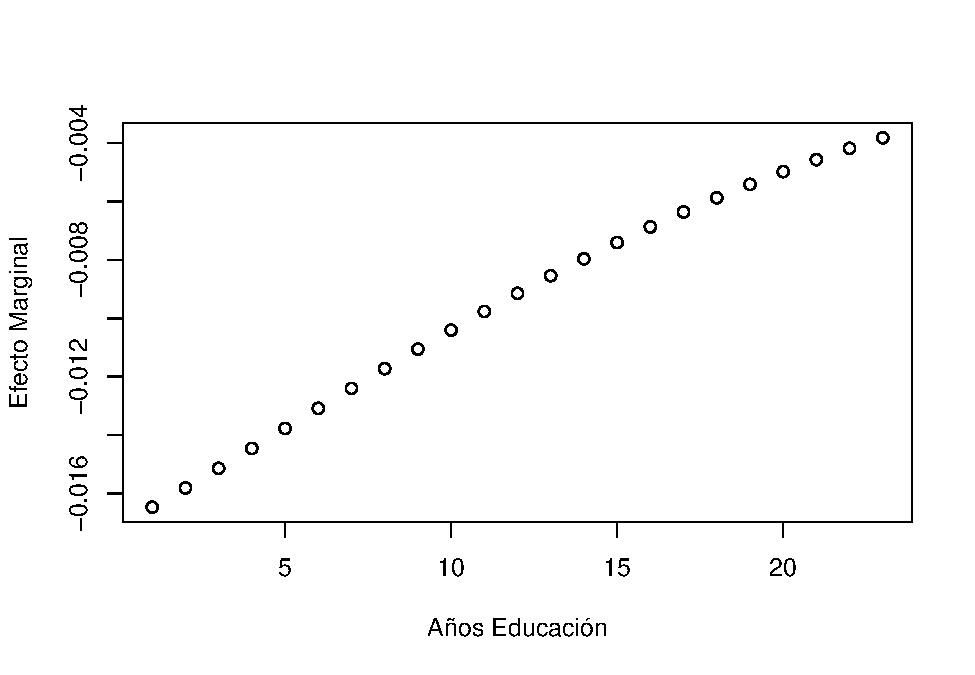
\includegraphics{_main_files/figure-latex/unnamed-chunk-94-1.pdf}

Una forma más directa de graficar los efectos marginales es a partir del comando \texttt{cplot} de la familia margins, que estima automaticamente estos mismos valores a partir de la estimación del modelo probit

\begin{Shaded}
\begin{Highlighting}[]
\CommentTok{\#cplot(probit, "aedu", what = "effect", main = "Average Marginal Effect of Weight")}
\end{Highlighting}
\end{Shaded}


  \bibliography{book.bib,packages.bib}

\end{document}
